\label{chap:rt}
\def \imgpath {"./figures/rt"}

In this chapter, measurements of \KOs, \LA, and \AL are reported as a function of the underlying event activity classifiers \RT, \RTmin, and \RTmax. These observables quantify the magnitude of the underlying event and are an experimental proxy of the number of Multiple Partonic Interactions, \nmpi.

\section{Motivation for studying event sub-structure}

\subsection{Underlying event}

As discussed in Section~\ref{sec:intro:ue}, the underlying event is composed of particles that are not directly related to the primary hard scattering and its related fragmentation. It can be studied to extract accurate information about the hard scattering process by subtracting it in precision measurements of jet properties. Moreover, since it is a manifestation of the proton substructure and the parton interactions, it can give us insight into the parton dynamics in the nonperturbative QCD region.

%In theory chapter, discuss UE history:
%J. R. Cudell et al., "Experimental study of the underlying event in high transverse momentum jet production at the CERN ISR", Nuclear Physics B, Volume 336, Issue 1, Pages 1-21 (1990). DOI: 10.1016/0550-3213(90)90568-V
%CDF Collaboration, "Observation of the Underlying Event in Dijet Events with a Leading Transverse Energy Jet at the Collider Detector at Fermilab", Physical Review Letters, Volume 83, Issue 7, Pages 1183-1188 (1999). DOI: 10.1103/PhysRevLett.83.1183
%DELPHI Collaboration, "Measurement of the underlying event in hadronic Z0 decays", Physics Letters B, Volume 382, Issues 3–4, Pages 323-332 (1996). DOI: 10.1016/0370-2693(96)00620-1

\subsection{Hard process--multiplicity bias}

Studying QGP phenomena in small systems as a function of event activity is challenging due to selection biases that arise when analyzing the data. It is known that selecting events with large momentum transfer leads to a bias towards higher multiplicities (and underlying event) \cite{alicecollaborationConstraintsJetQuenching2018}, and conversely, selecting events with higher multiplicities (and UE) enhances the hard processes \cite{alicecollaborationMultiplicityDependenceChargedparticle2022}. This bias can be understood in several ways. Firstly, a hard process tends to occur with lower impact parameters, which in turn leads to higher particle multiplicities. Secondly, an event with $n$ partonic interactions has $n$ chances of containing a hard process. Lastly, harder processes fragment into more particles, further contributing to higher event activity. As an example, Figure~\ref{fig:rt:hardbias} shows how the requirement of a high \pt track can skew the forward-rapidity centrality distribution to lower values (higher event activity), as observed in a result from ALICE \cite{alicecollaborationConstraintsJetQuenching2018}.

\begin{figure}%
\subfloat[][]{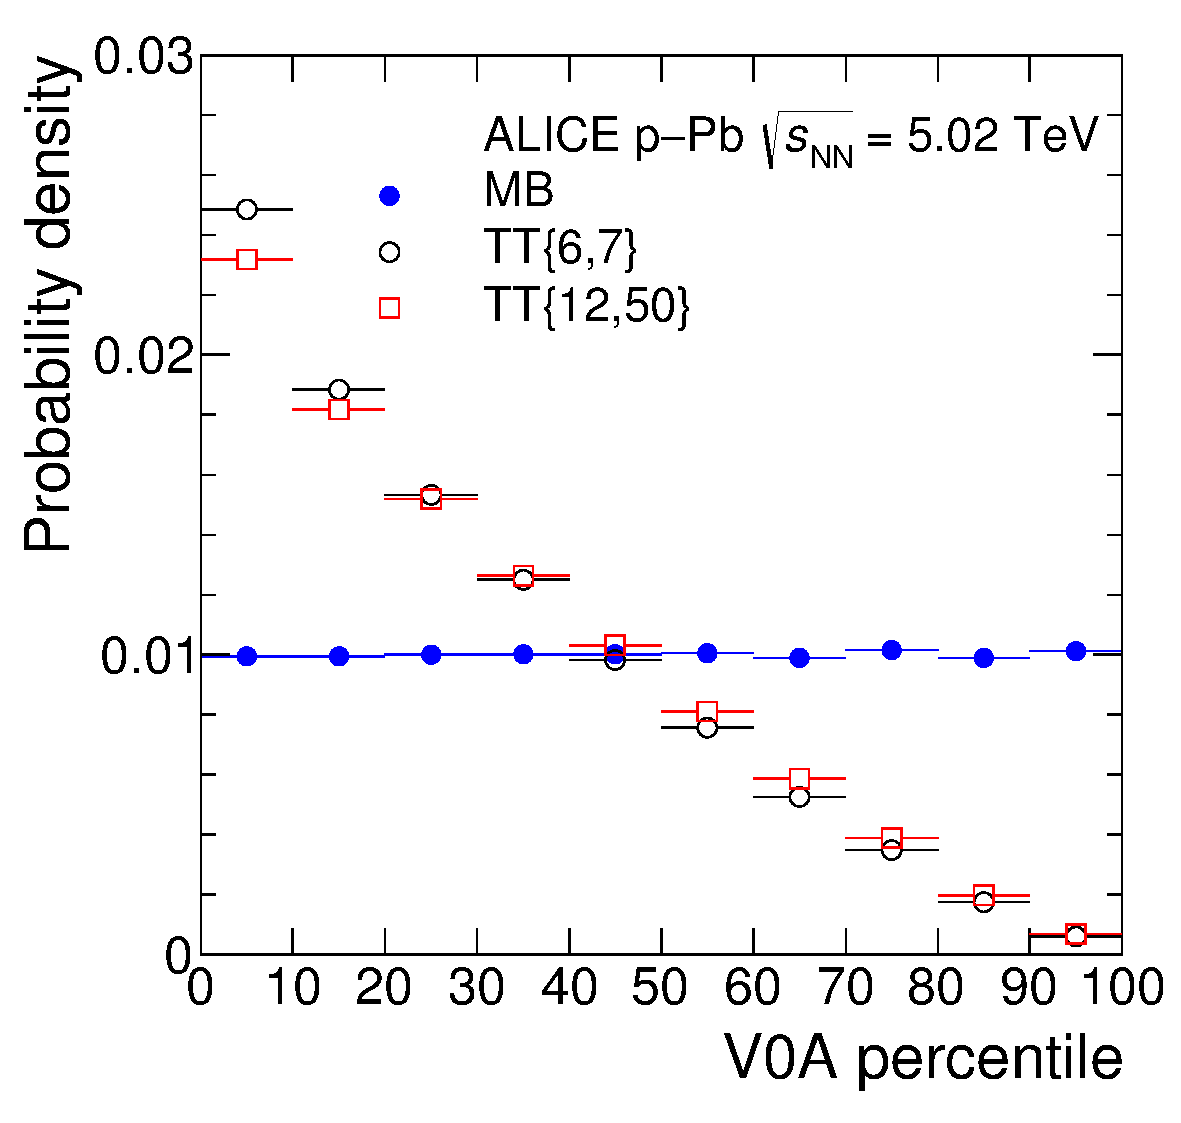
\includegraphics[width=.480\textwidth]{\imgpath/alice_hard_multi_bias.pdf}}\\
\caption{Distribution of event activity measured at forward rapidity (\VOA percentile) for minimum bias events (blue points) and for events requiring a high-\pt trigger in the intervals $6<\pt<\gevc{7}$ (black points) and $12<\pt<\gevc{50}$ (red points). Lower \VOA percentile represent higher event activity. The MB distribution is trivally uniform by construction. \cite{alicecollaborationConstraintsJetQuenching2018}}
\label{fig:rt:hardbias}
\end{figure}

\subsection{Azimuthal regions and transverse activity}

The selection bias of hard processes on UE becomes saturated at high \pt, where the impact parameter bias is fixed and stochastic effects become comparable \cite{acharyaUnderlyingEventProperties2020}. This saturation effect can be observed when studying particle production in three topological regions defined with respect to the highest momentum track, which serves as a proxy for the axis of the primary scattering process. The three regions are defined as follows:
\begin{enumerate}
\item Towards (also known as "Near"), where $|\phi - \philead| < \frac{\pi}{3}$,
\item Away, where $|\phi - \philead| > \frac{2\pi}{3}$, and 
\item Transverse, where $\frac{\pi}{3} < |\phi - \philead| < \frac{2\pi}{3}$. 
\end{enumerate}
Here, \philead is the azimuthal angle of the leading track. This definition is illustrated in Figure~\ref{fig:rt:rtdefi}. 

\begin{figure}%
\subfloat[][]{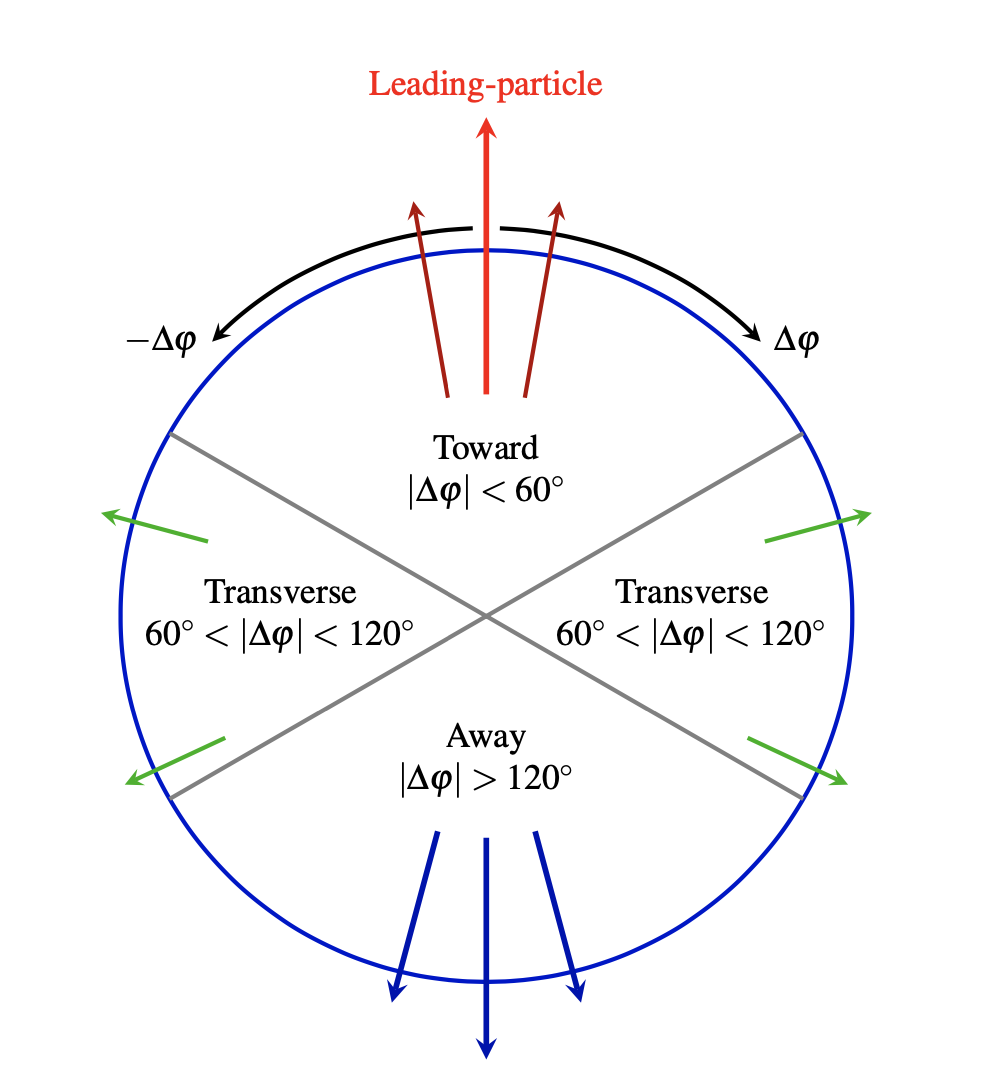
\includegraphics[width=.490\textwidth]{\imgpath/rt_defi.png}}
\subfloat[][]{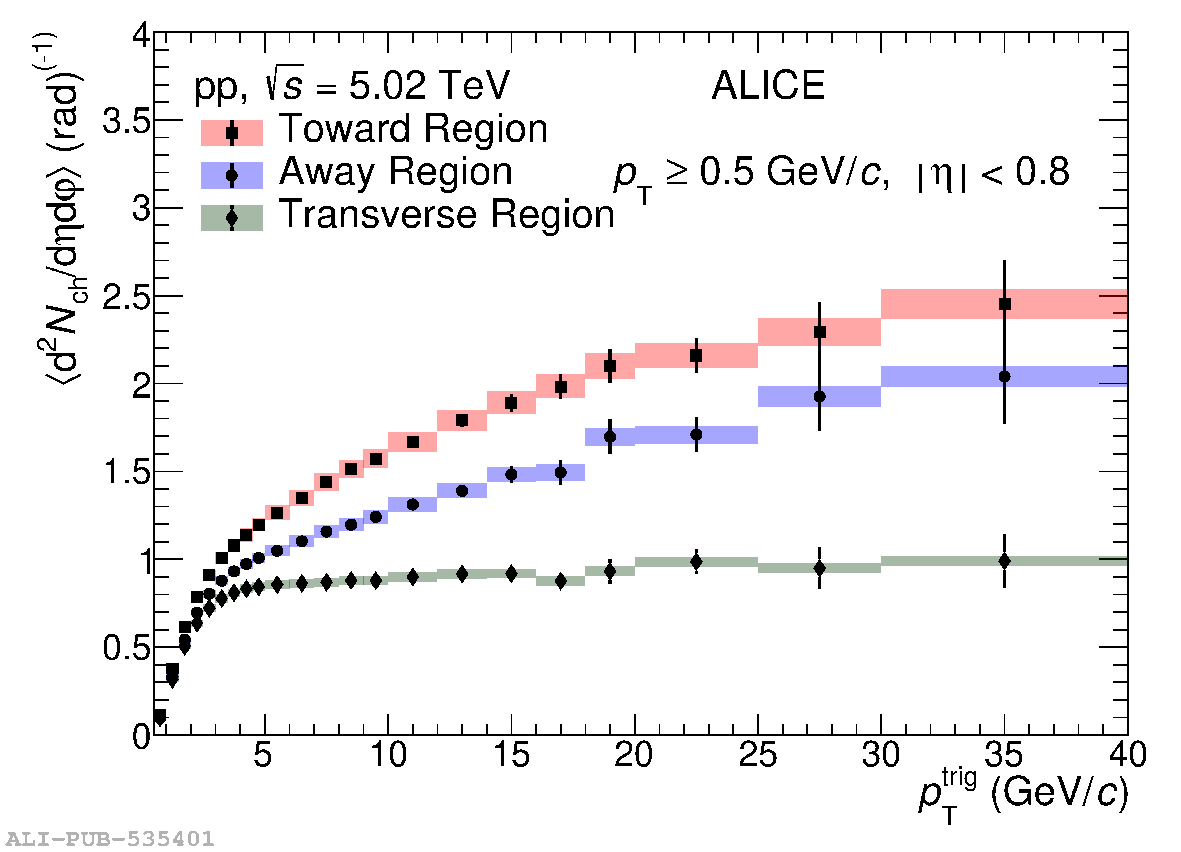
\includegraphics[width=.490\textwidth]{\imgpath/alice_uevpt.pdf}}\\
\caption{\textbf{(a)} Illustration of the three azimuthal regions: Toward, Away, Transverse; defined with respect to the highest-\pt track. \cite{acharyaUnderlyingEventProperties2020} \textbf{(b)} Charged particle density distributions as a function of \pt of the leading track in the three azimuthal regions. Error bars indicate statistical uncertainties and shaded areas represent systematic uncertainties. \cite{acharyaUnderlyingEventProperties2020} }
\label{fig:rt:rtdefi}
\end{figure}

Studying particle multiplicity (or sum of their \pt) in these regions as a function of the transverse momentum of the leading track \ptlead reveals that in the regions Towards and Away, the multiplicity continues to increase with the hardness of the primary process \cite{acharyaUnderlyingEventProperties2020, atlascollaborationMeasurementChargedparticleDistributions2017}. These regions contain the leading and the recoil jet, respectively. In contrast, in the Transverse region, the multiplicity (further denoted as $N_T$ in this thesis but $N_\mathrm{ch}^\mathrm{trans}$ is also used in cited literature) reaches a plateau at around $\gevc{5}$. In this region, the underlying event becomes independent of the strength of the primary process, and the selection bias is minimized. Notably, this phenomenon is universal regardless of the system size or collision energy \cite{atlascollaborationMeasurementChargedparticleDistributions2017, acharyaUnderlyingEventProperties2020, alicecollaborationUnderlyingEventMeasurements2012, alicecollaborationUnderlyingeventPropertiesPp2022}. As an example, measurements from ALICE are shown in Fig.~\ref{fig:rt:rtdefi}.

\section{\RT as an experimental observable}

The magnitude of the underlying event can be measured using the self-normalized ratio:
\begin{align}
\RT = \frac{\NT}{\langle \NT \rangle},
\end{align}
which is often referred to as the underlying event activity, transverse activity, or relative transverse activity in various literature \cite{martinProbingCollectiveEffects2016, alicecollaborationUnderlyingEventProperties2020, alicecollaborationProductionPionsKaons2023}, and also in this thesis. This observable and its uses were suggested in Ref.~\cite{martinProbingCollectiveEffects2016}.

By applying $\RT$, two limits of events can be studied:
\begin{itemize}
\item $\RT \rightarrow 0$: the \textbf{``ee"} limit, where events with minimal UE are selected. These events are dominated by a single hard scattering and can be compared to LEP fragmentation models.
\item $\RT \rightarrow \infty$: the \textbf{``AA"} limit, where events with very high transverse activity are selected, which can come from many MPIs and/or from transverse jets. These events may exhibit features similar to pA and AA collisions.
\end{itemize}

\subsection{Proxy to \nmpi}

As could be intuitively expected, \RT serves as an experimental proxy for \meannmpi. Phenomenological models that incorporate MPIs provide an illustration of this relationship. As shown in Fig.~\ref{fig:rt:nmpi}, Pythia 8 predicts a strong dependence of \meannmpi on \RT until $\RT \lesssim 5$. Similarly, Herwig 7 predicts a dependence until $\RT \lesssim 3$, albeit weaker. Pythia's prediction for the relationship between \RT and the event multiplicity, which is affine, is also shown in Fig.~\ref{fig:rt:nmpi}.

\begin{figure}%
\subfloat[][]{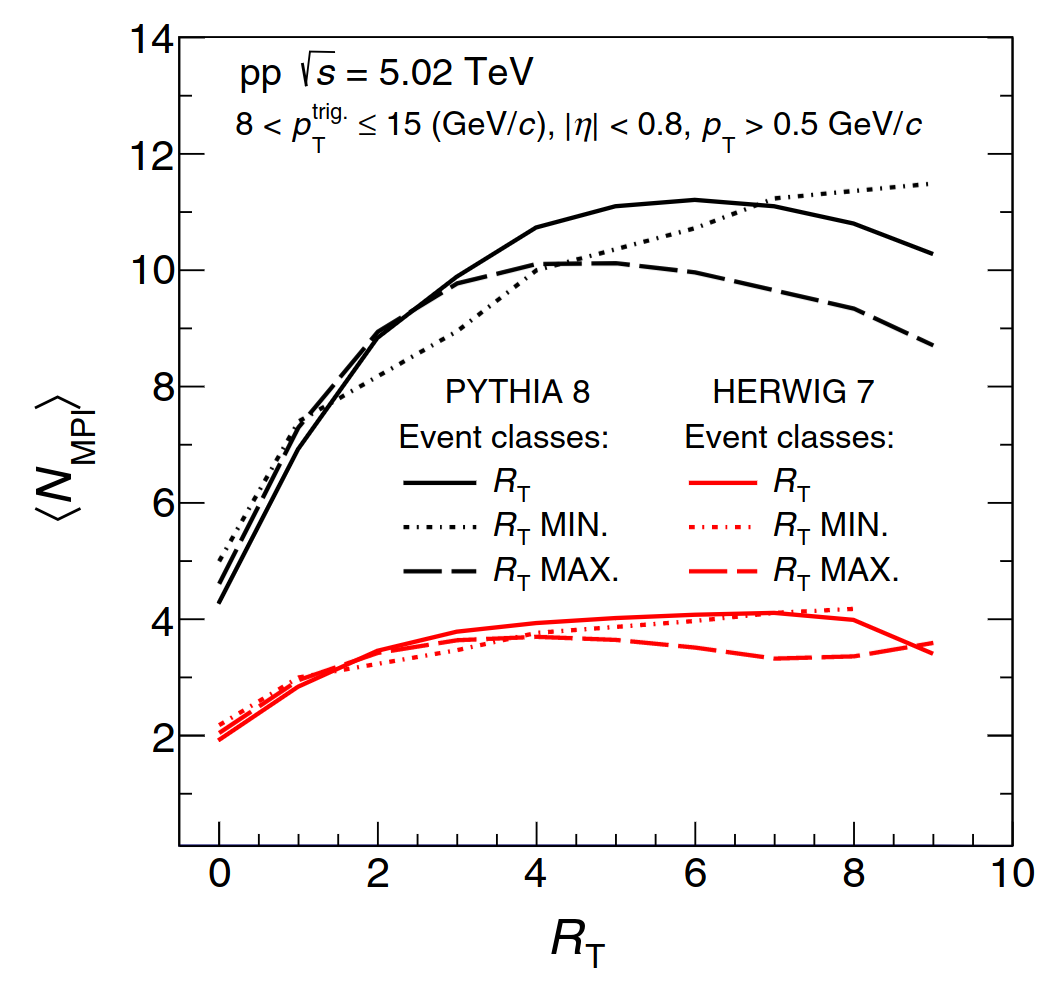
\includegraphics[width=.480\textwidth]{\imgpath/rt_minmax_nmpi.png}}
\subfloat[][]{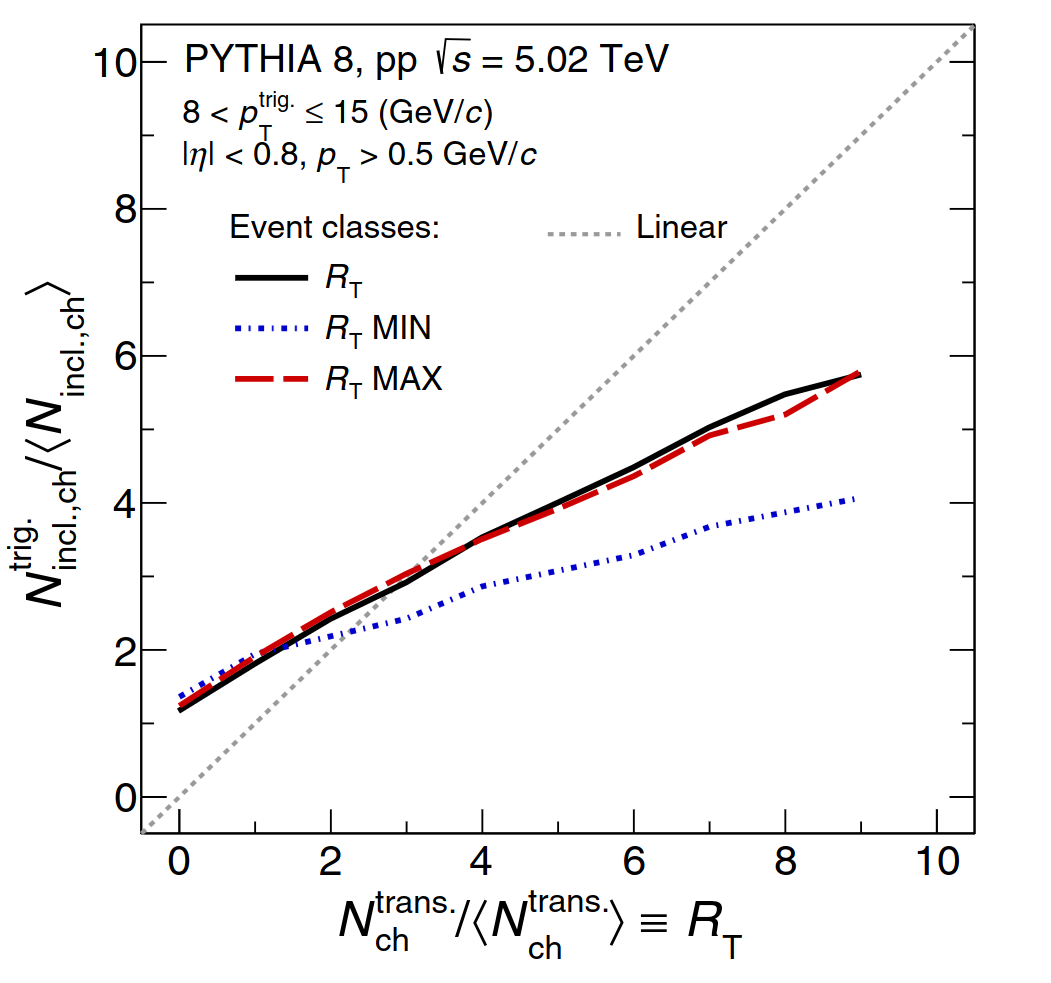
\includegraphics[width=.465\textwidth]{\imgpath/rt_nch.png}}\\
\caption{\textbf{(a)} Dependence of the mean number of MPIs on the underlying event activity classifiers \RT, \RTmin, and \RTmax in pp collisions at \sppt{5.02}, as predicted by Pythia 8 (black) and Herwig 7 (red). \cite{bencediDisentanglingHardGluon2021} \textbf{(b)} Pythia 8 prediction for the correlation of the self-normalised charged particle multiplicity measured at mid-rapidity in events with a high-\pt trigger and the underlying event activity classifiers \RT, \RTmin, \RTmax. \cite{bencediDisentanglingHardGluon2021}}
\label{fig:rt:nmpi}
\end{figure}


\subsection{Extension to \RTmin, \RTmax}

Upon closer inspection of Fig.~\ref{fig:rt:rtdefi}, it can be observed that the charged particle multiplicity does not completely plateau in the Transverse region either, which was an important factor in motivating \RT measurements. Instead, there is a slight increase with \ptlead, although the effect is small. This rise can be attributed to harder, wide-angle ISR and FSR \cite{fieldUnderlyingEventHadronic2012}.

To separate the soft and hard components of the underlying event -- namely, the MPIs from wide-angle ISR/FSR -- the definition of \RT can be extended. The two transverse sub-regions can be further classified as Transverse-min or Transverse-max, based on which sub-region has fewer or more particles. Softer contributions from MPIs will enter both sub-regions, whereas harder radiation should affect mainly the Transverse-max sub-region. This makes Transverse-min more sensitive to particle production from MPIs. Figure~\ref{fig:rt:ue} illustrates how the Transverse-max region captures most of the rise of \meanNch and \meanpt, whereas the Transverse-min region is much closer to plateauing.

\begin{figure}%
\subfloat[][]{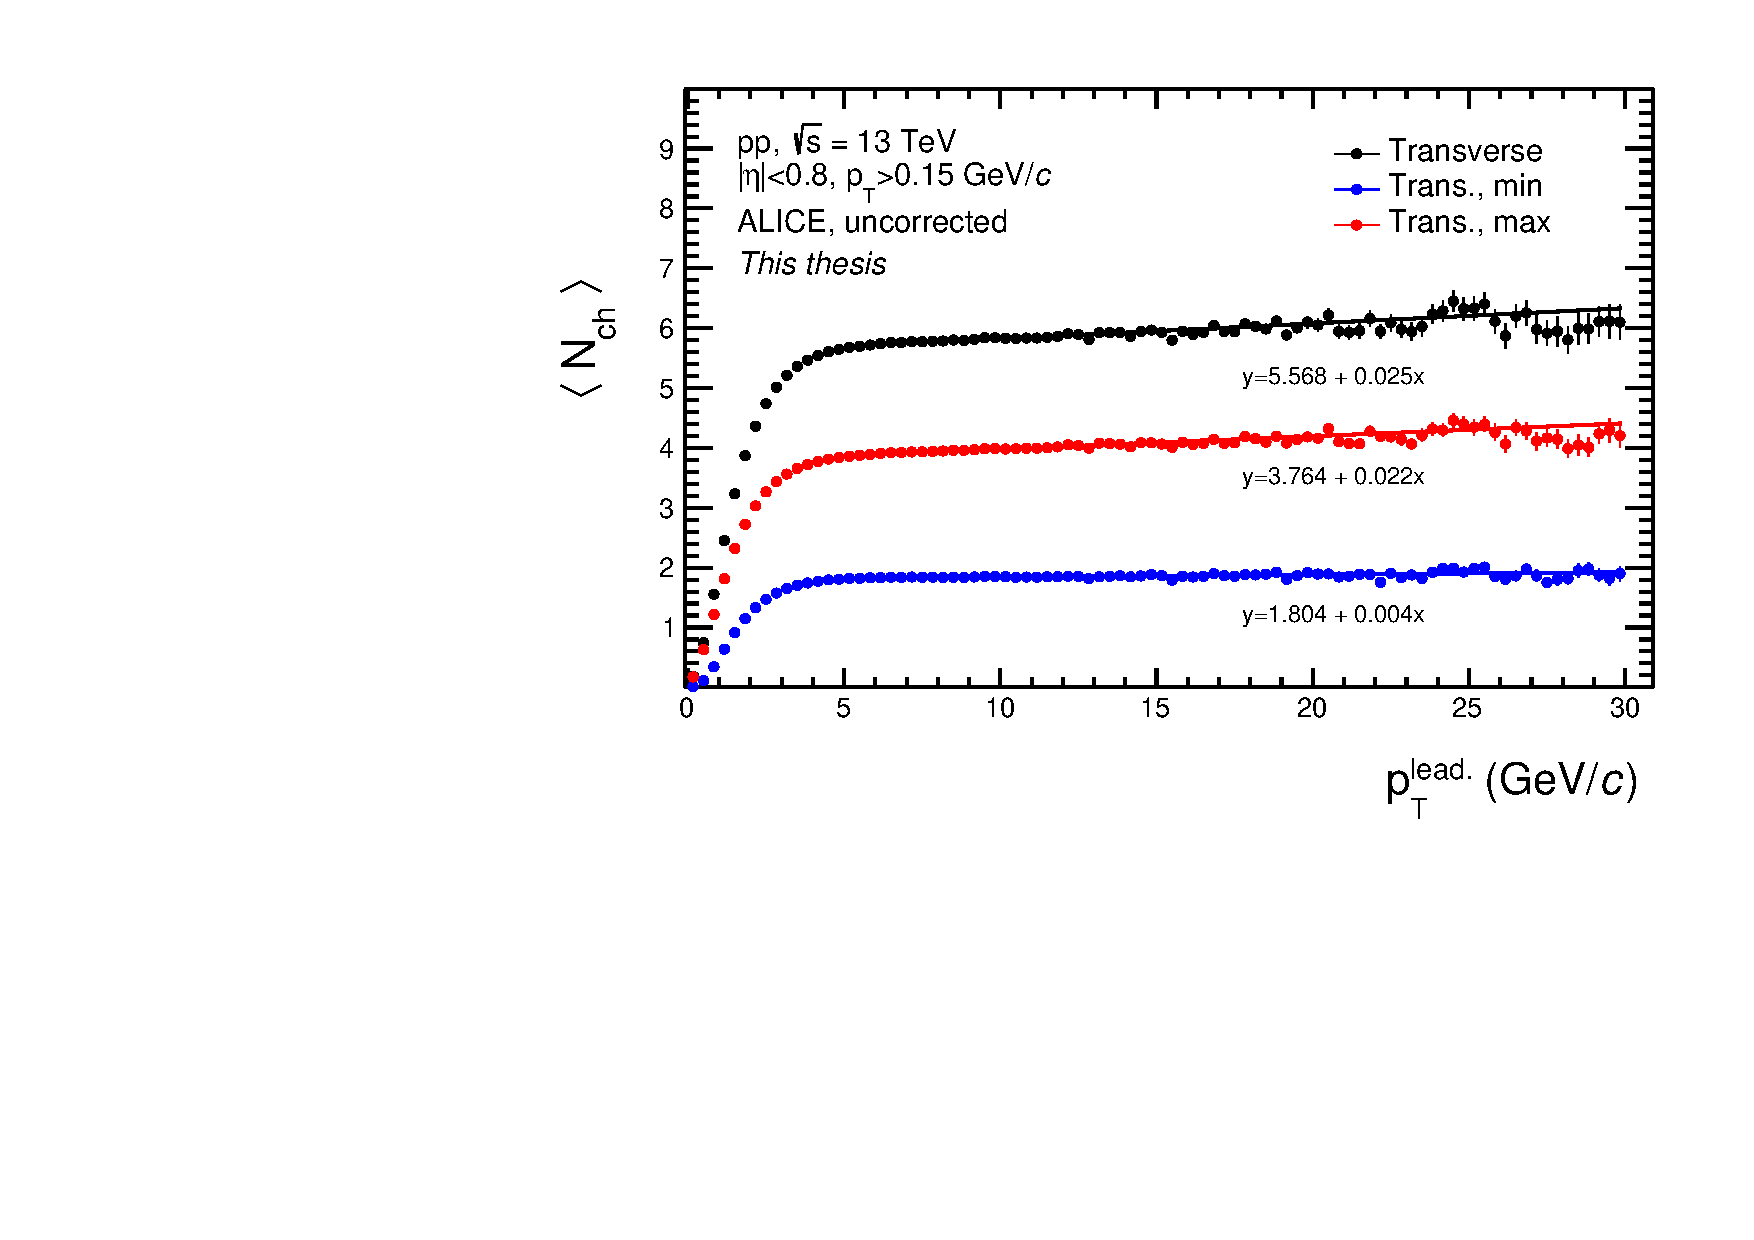
\includegraphics[width=.490\textwidth]{\imgpath/InfoRT_UE0.pdf}}
\subfloat[][]{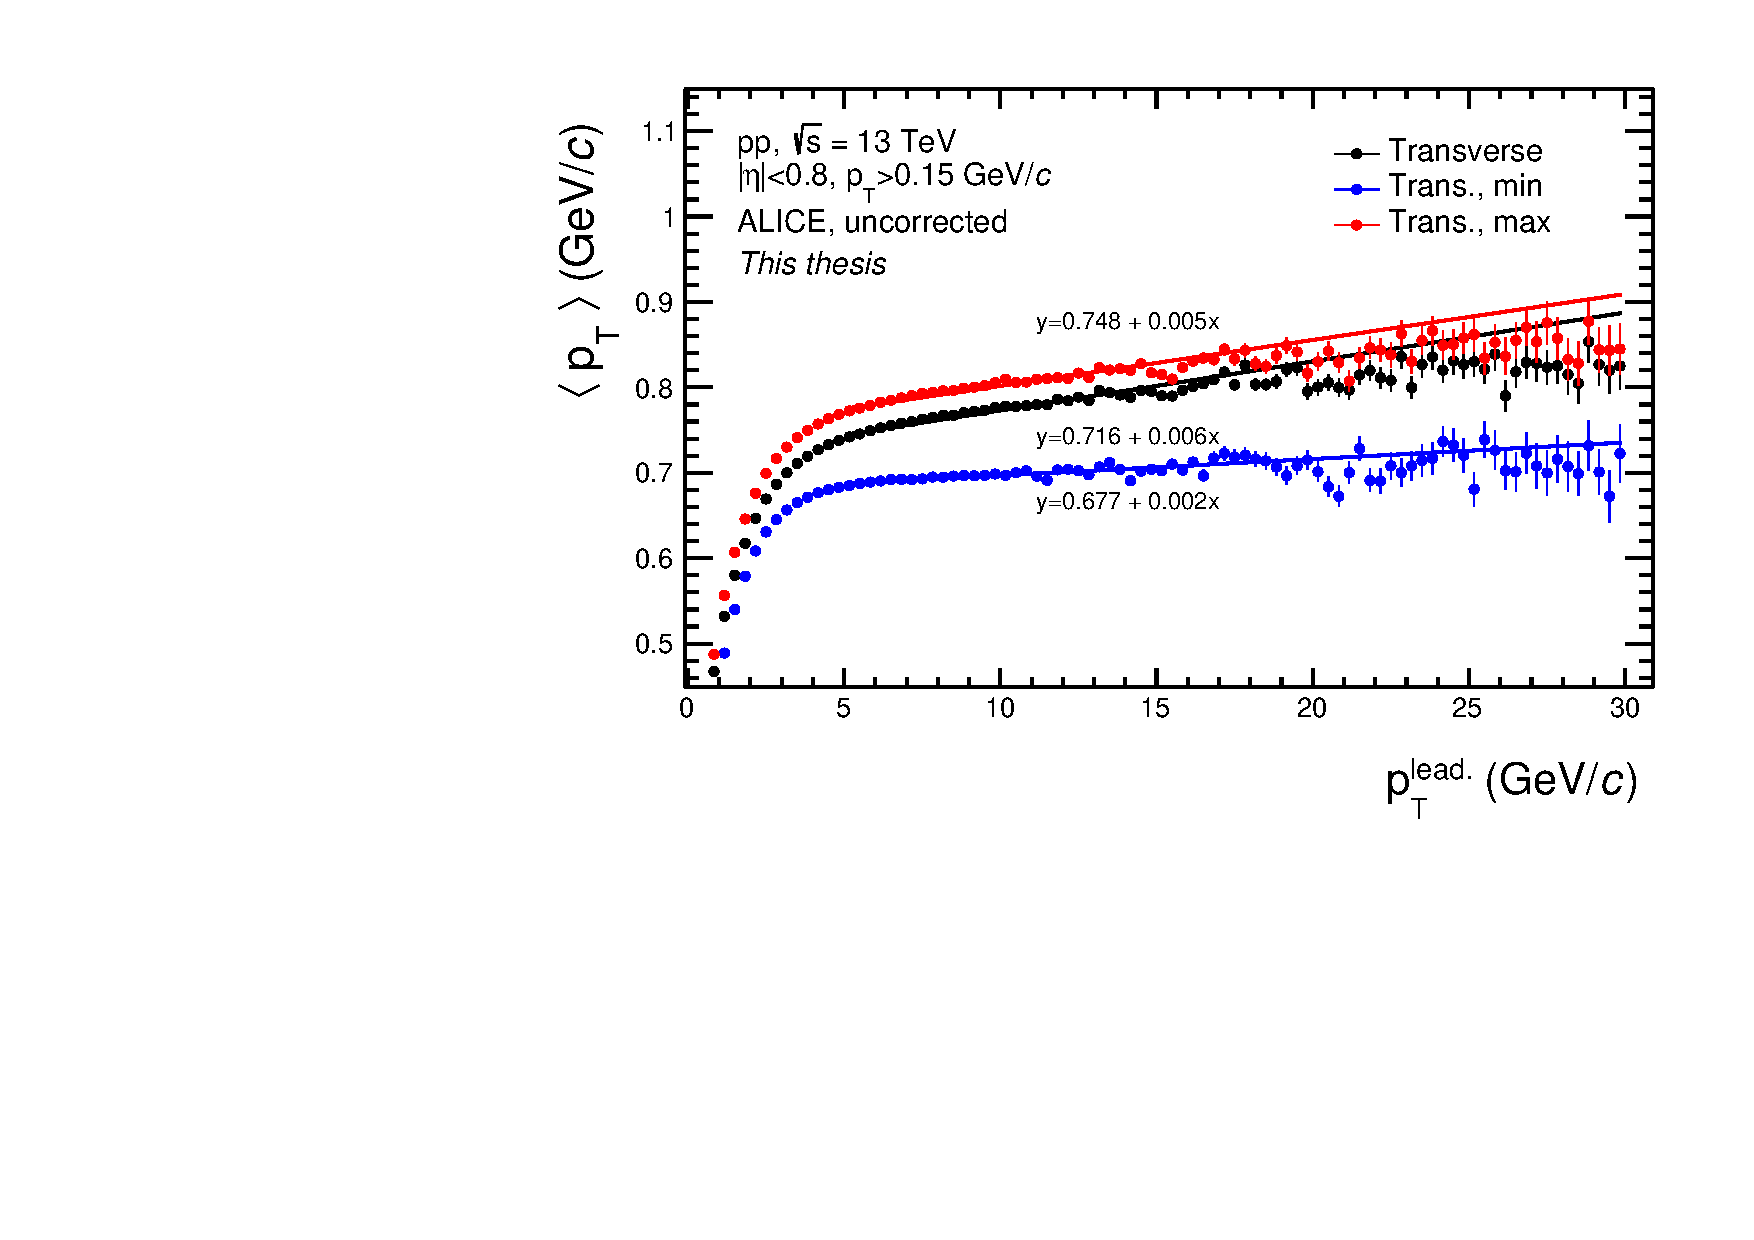
\includegraphics[width=.490\textwidth]{\imgpath/InfoRT_UE1.pdf}}
\caption{TBA}
\label{fig:rt:ue}
\end{figure}

Analogously, the following underlying event activity classifiers can be defined:
\begin{align}
\RTmin &= \frac{\NTmin}{\langle \NTmin \rangle} \quad, \\
\RTmax &= \frac{\NTmax}{\langle \NTmax \rangle} \quad,
\end{align}
where \NTmin and \NTmax are the particle multiplicities in the Transverse-min and Transverse-max sub-regions, respectively. This approach follows measurements developed at UE studies at Tevatron \cite{fieldUnderlyingEventHadronic2012} and has been suggested to use in searches for QGP phenomena in small systems based on investigations in phenomenological models \cite{bencediDisentanglingHardGluon2021}. In the rather rare situations with $\NTmin = \NTmax$, the classification is based on the sum of \pt instead.

According to Pythia 8, as shown in Fig.~\ref{fig:rt:nmpi}, \RTmin and \RTmax follow different relationships with \meannmpi. Whereas \meannmpi starts falling as a function of \RTmax (due to the inclusion of mini-jets) at $\RTmax \approx 5$, it continues rising as a function of \RTmin across the entire range. Furthermore, compared to \RT, \RTmin also shows some degree of decorrelation with event multiplicity.


\subsubsection{Charged particle \pt spectra}

Phenomenological models also reveal a different evolution of transverse momentum spectra of inclusive charged particles based on \RTmin and \RTmax, as shown in Fig.~\ref{fig:rt:nchpt}. For the highest reported ranges of \RTmax and \RT, a significant hardening of the spectrum is observed in both Pythia 8 and Herwig 7, similarly to multiplicity studies \cite{alicecollaborationMultiplicityDependenceLightflavor2019}, indicating a strong auto-correlation. In contrast, \RTmin exhibits a Cronin-like enhancement\footnote{Cronin effect refers to the modification of \pt spectra in nuclear collisions as a result of partonic scattering in the nuclear medium and can be observed as a characteristic peak in nuclear modification factors at intermediate \pt \cite{kopeliovichCroninEffectHadron2002}.} at intermediate \pt and a plateau at $\pt \gtrsim \gevc{6}$, even in the highest \RTmin bin \cite{bencediDisentanglingHardGluon2021}. So far, this behaviour has not been observed in data.

\begin{figure}%
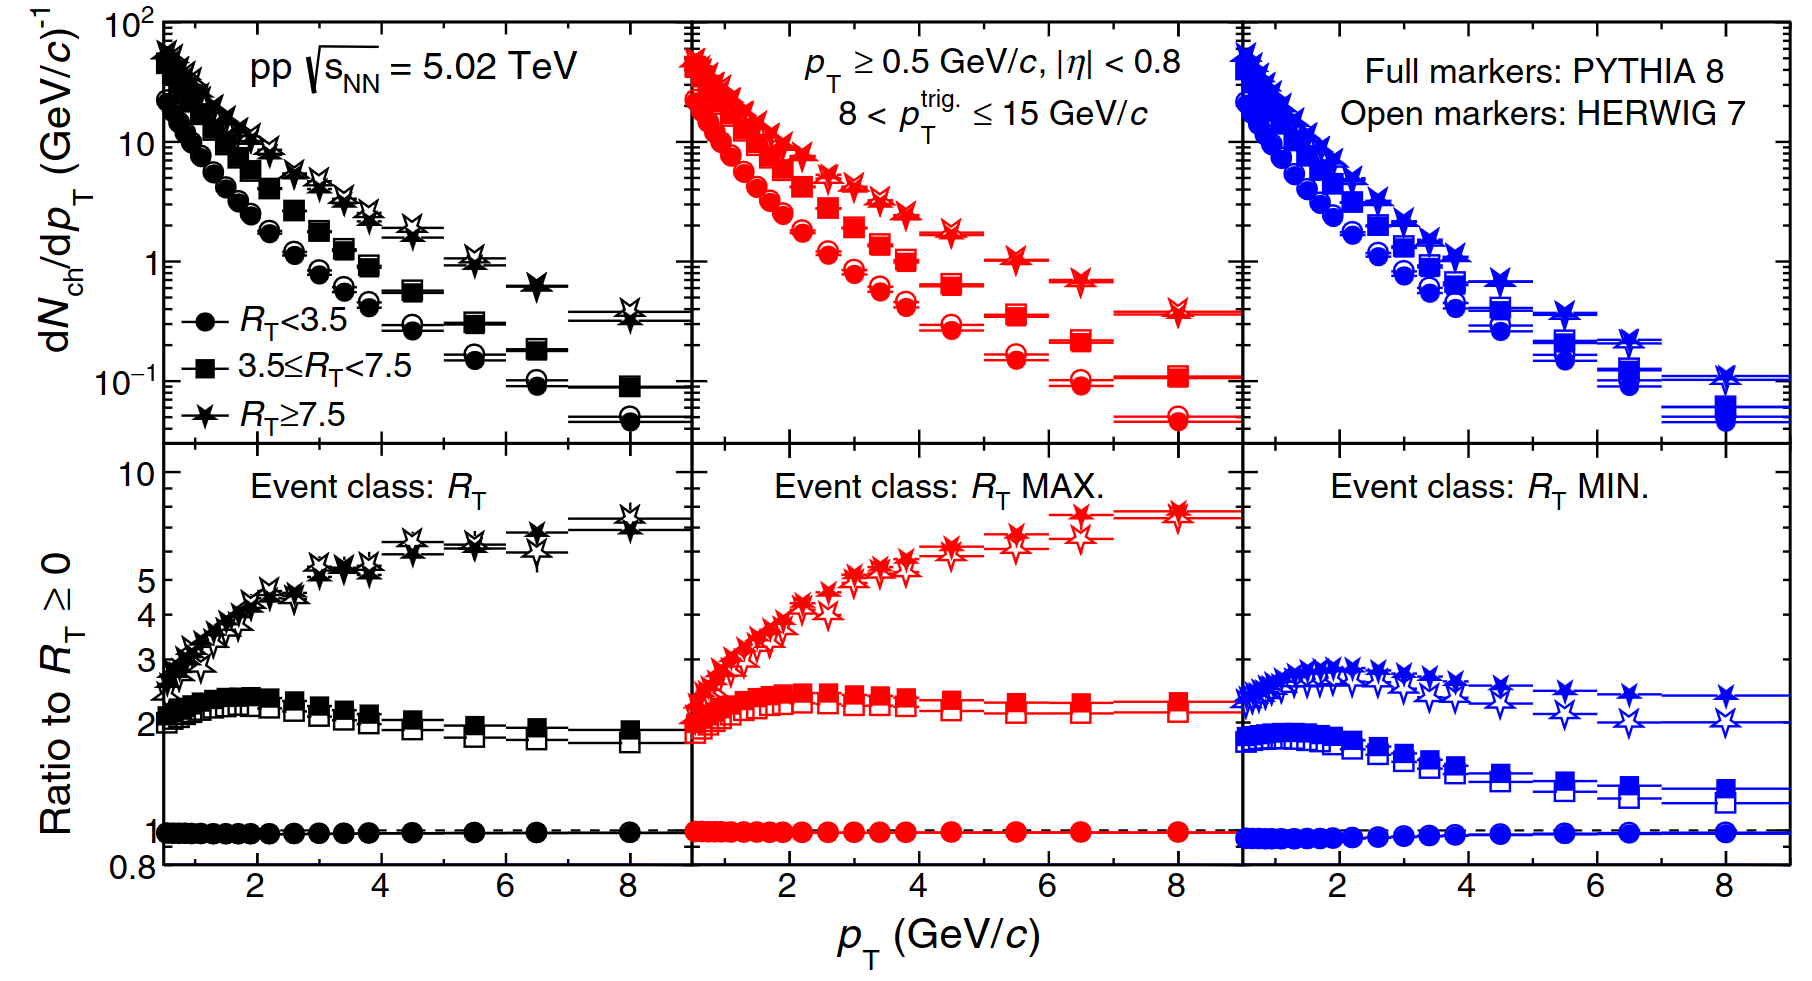
\includegraphics[width=.980\textwidth]{\imgpath/rt_nchpt.png}
\caption{Transverse momentum spectra of charged particles produced in three azimuthal regions: \textbf{(left)} Transverse, \textbf{(middle)} Transverse-max, \textbf{(right)} Transverse-min, as a function of the underlying event activity \RT/\RTmax/\RTmin in pp collisions at \sppt{5.02}. The bottom row displays the ratios to the UE-activity integrated cases. The predictions are based on Pythia 8 and Herwig 7 simulations. \cite{bencediDisentanglingHardGluon2021}}
\label{fig:rt:nchpt}
\end{figure}

\subsection{Track and event selection}

The event selection follows the same criteria as the \SOPT measurement discussed in Section~\ref{sec:sphero:eventtracks}, which conform to the standard analysis of light flavour hadrons versus multiplicity in pp collisions conducted in ALICE. The \INELgtO events, which require at least one hit in either \VOA or \VOC scintillators and a track reconstructed within $|\eta|<1$, are used. The SPD is used for the reconstruction of the primary vertex, which is further required to be close to the nominal vertex ($|\Delta z|<10$~cm) to reject out-of-bunch pile-up. To remove in-bunch pile-up, events with multiple reconstructed vertices are excluded.

Events are required to have a leading track with reconstructed momentum $5 < \ptlead$ $< \gevc{40}$\footnote{Note that \pt spectrum is falling very steeply, at an approximately exponential rate, making the upper bound negligibly restrictive compared to the lower bound.}. These values were chosen to access the plateau in transverse activity and isolate the UE while retaining a large data sample. Maintaining a high momentum and spatial resolution of the leading track is crucial in this measurement. However, this can be compromised at high \pt when a significant portion of the track curvature can fall between two sectors of the TPC. To address this issue, geometrical cuts are used, as discussed in Section~\ref{TBA}.

For both the leading particle as well as the particles entering \NT and \RT calculations, tracks are required to be within $|\eta|<0.8$ and have $\pt > \gevc{0.15}$, and must satisfy the following:
\begin{enumerate}
\item ``Hybrid tracks", described in more detail in Section~\ref{chap:tracks}, are used for both leading and \NT tracks to ensure a high level of azimuthal acceptance uniformity. These tracks consist of high-quality ``global track" requirements, including the SPD information, which leads to azimuthal non-uniformity, and ``complementary track" cuts, a looser set requiring only ITS and TPC in cases where the first are not satisfied.
\item  For the leading track, strict \pt-dependent DCA cuts are applied in the transverse direction ($|\mathrm{DCA}_{xy}| < 0.0182 + \frac{0.0350}{\pt^{1.01}}$~cm, $\pt \in [ \mathrm{\gevc} ]$), to ensure good momentum resolution and that the track is a primary one.
\item For the \NT tracks, a DCA cut ($|\mathrm{DCA}_{xy}| < 0.06$~cm) is required to avoid biases in \VO measurements, as explained in the text below.
\end{enumerate}

\subsection{\RT measurements of neutral particles vs. charged particles}

The \VOs are neutral particles and thus, they cannot be leading tracks nor enter \NT (\NTmin, \NTmax) and \RT (\RTmin, \RTmax) calculations. This has several implications:
\begin{enumerate}
\item \VOs suffer much less from auto-correlation biases than \pikp, which can be seen in azimuthal distributions and in $\KOs / \mathrm{K}^\pm$ ratios. Requiring high/low \NT/\RT can lead to an increase/decrease of charged particles in the Transverse region due to selecting fluctuations in addition to the UE scaling. However, this effect is significantly smaller for neutral \VOs. This behaviour is shown in Fig.~\ref{fig:rt:autocorr}. It is important to bear this caveat in mind when comparing \pt spectra and yields of \pikp and \VOs.
\item While \NT is always at least $1$ for \pikp in the Transverse region, for \VOs it can be equal to $0$. Similar logic applies to the Transverse-min/max sub-regions and \NTmin/\NTmax .
\item The maximum \pt measurable for \pikp in the Toward region is limited to $\pt < \gevc{5}$, at which point the trigger requirement would lead to a trivial increase. For \VOs, however, this limitation does not apply and their measured \pt range does not need to be restricted.
\item The charged daughters of \VOs could sometimes enter \NT, leading to significant biases at low \pt in the Toward and Away regions of $\KOs/\mathrm{K}^\pm$ ratios. 
\end{enumerate} 

In this thesis, the behaviour described in the last point was rectified by making \NT track candidates and \VO daughter tracks two disjunct sets. This was achieved by applying the $|\mathrm{DCA}_{xy}|>0.06$~cm cut, used in the \VO reconstruction as discussed in Section~\ref{sec:ana:cuts}, in opposite ways. This reduces the \NT track candidates by less than $5\%$. The effect of this solution can be seen in Fig.~\ref{fig:rt:KtoK}.

\begin{figure}%
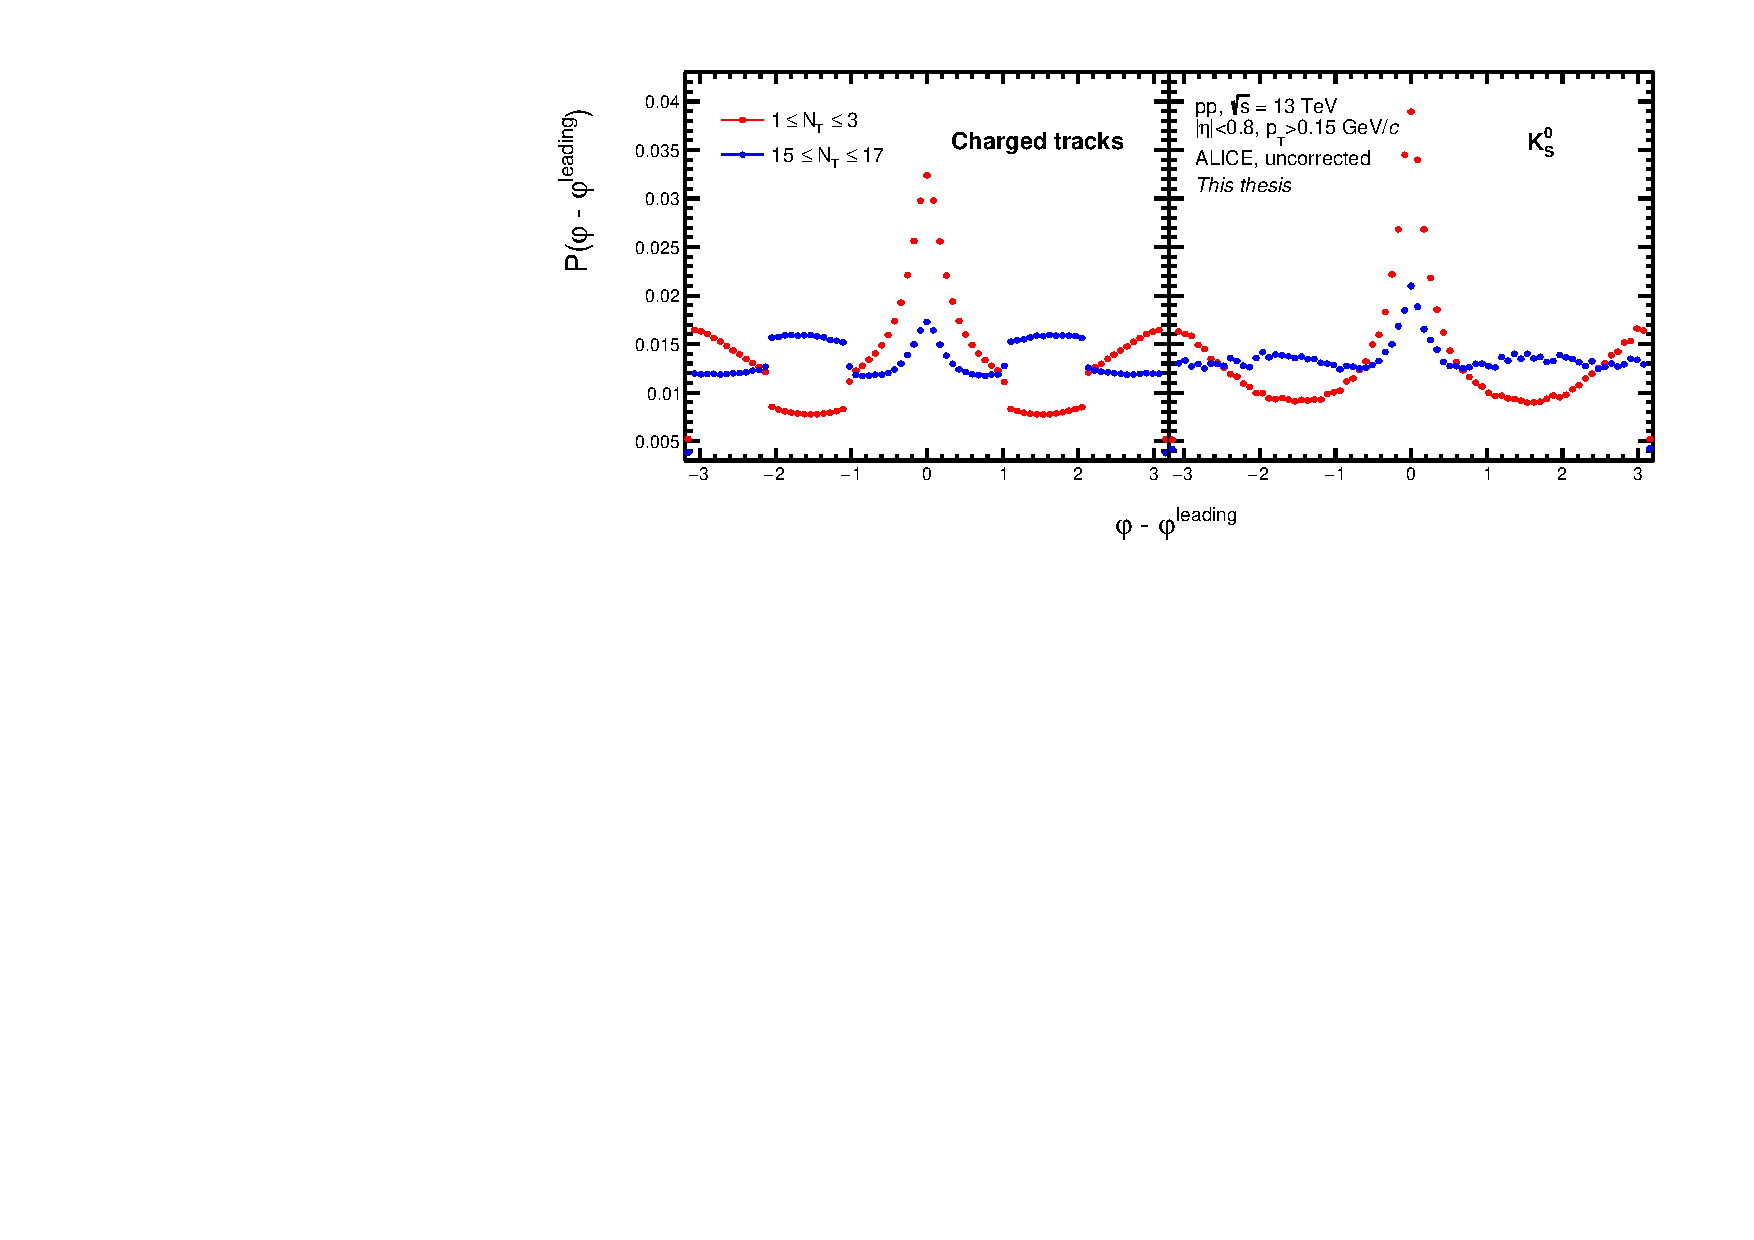
\includegraphics[width=.990\textwidth]{\imgpath/InfoRT_autocorr.pdf}\\
\caption{Probability distributions of the azimuthal angle of \textbf{(left)} charged tracks and \textbf{(right)} the neutral \KOs. Events with low \NT (red) and high \NT (blue) are compared. The results are uncorrected for reconstruction  effects and acceptance and show only statistical uncertainties.}
\label{fig:rt:autocorr}
\end{figure}


\begin{figure}%
\subfloat[][]{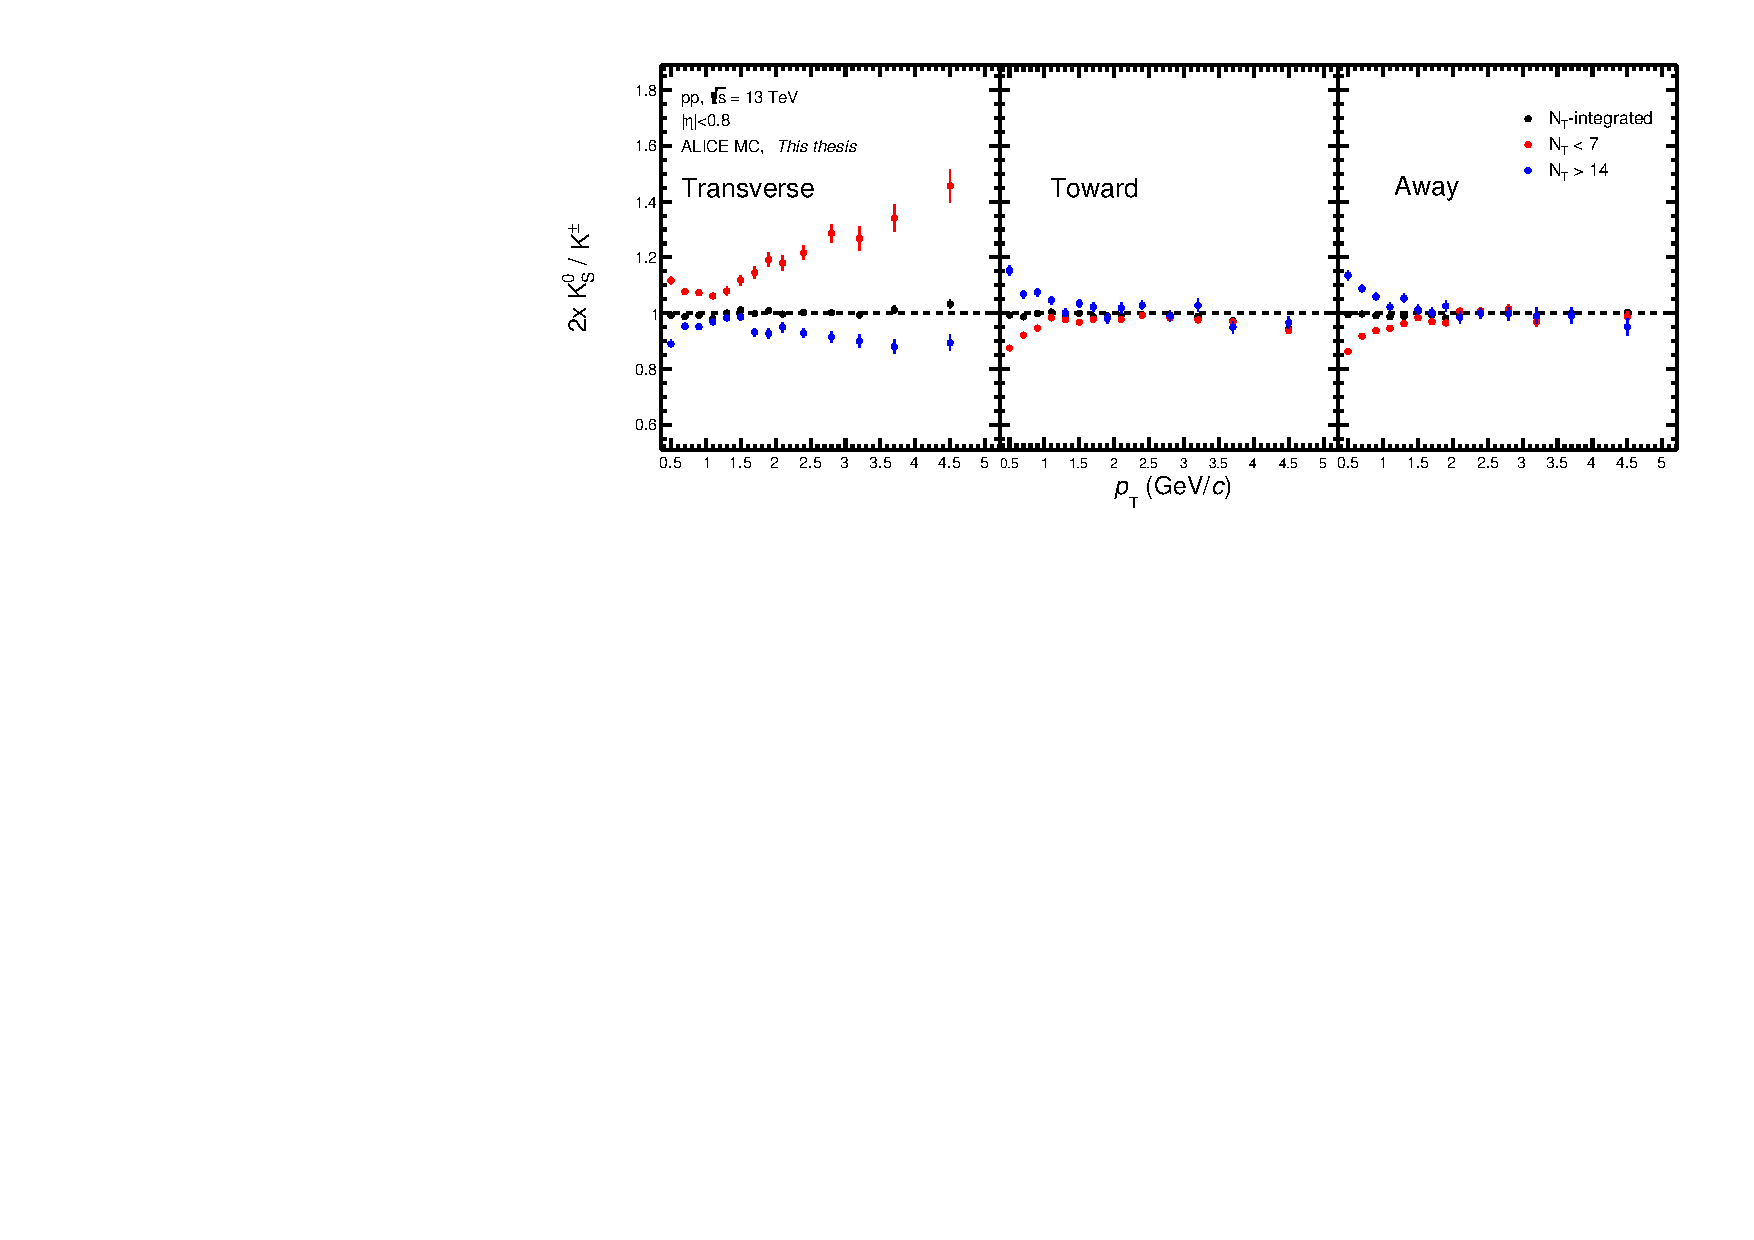
\includegraphics[width=.990\textwidth]{\imgpath/KtoK_old.pdf}}\\
\subfloat[][]{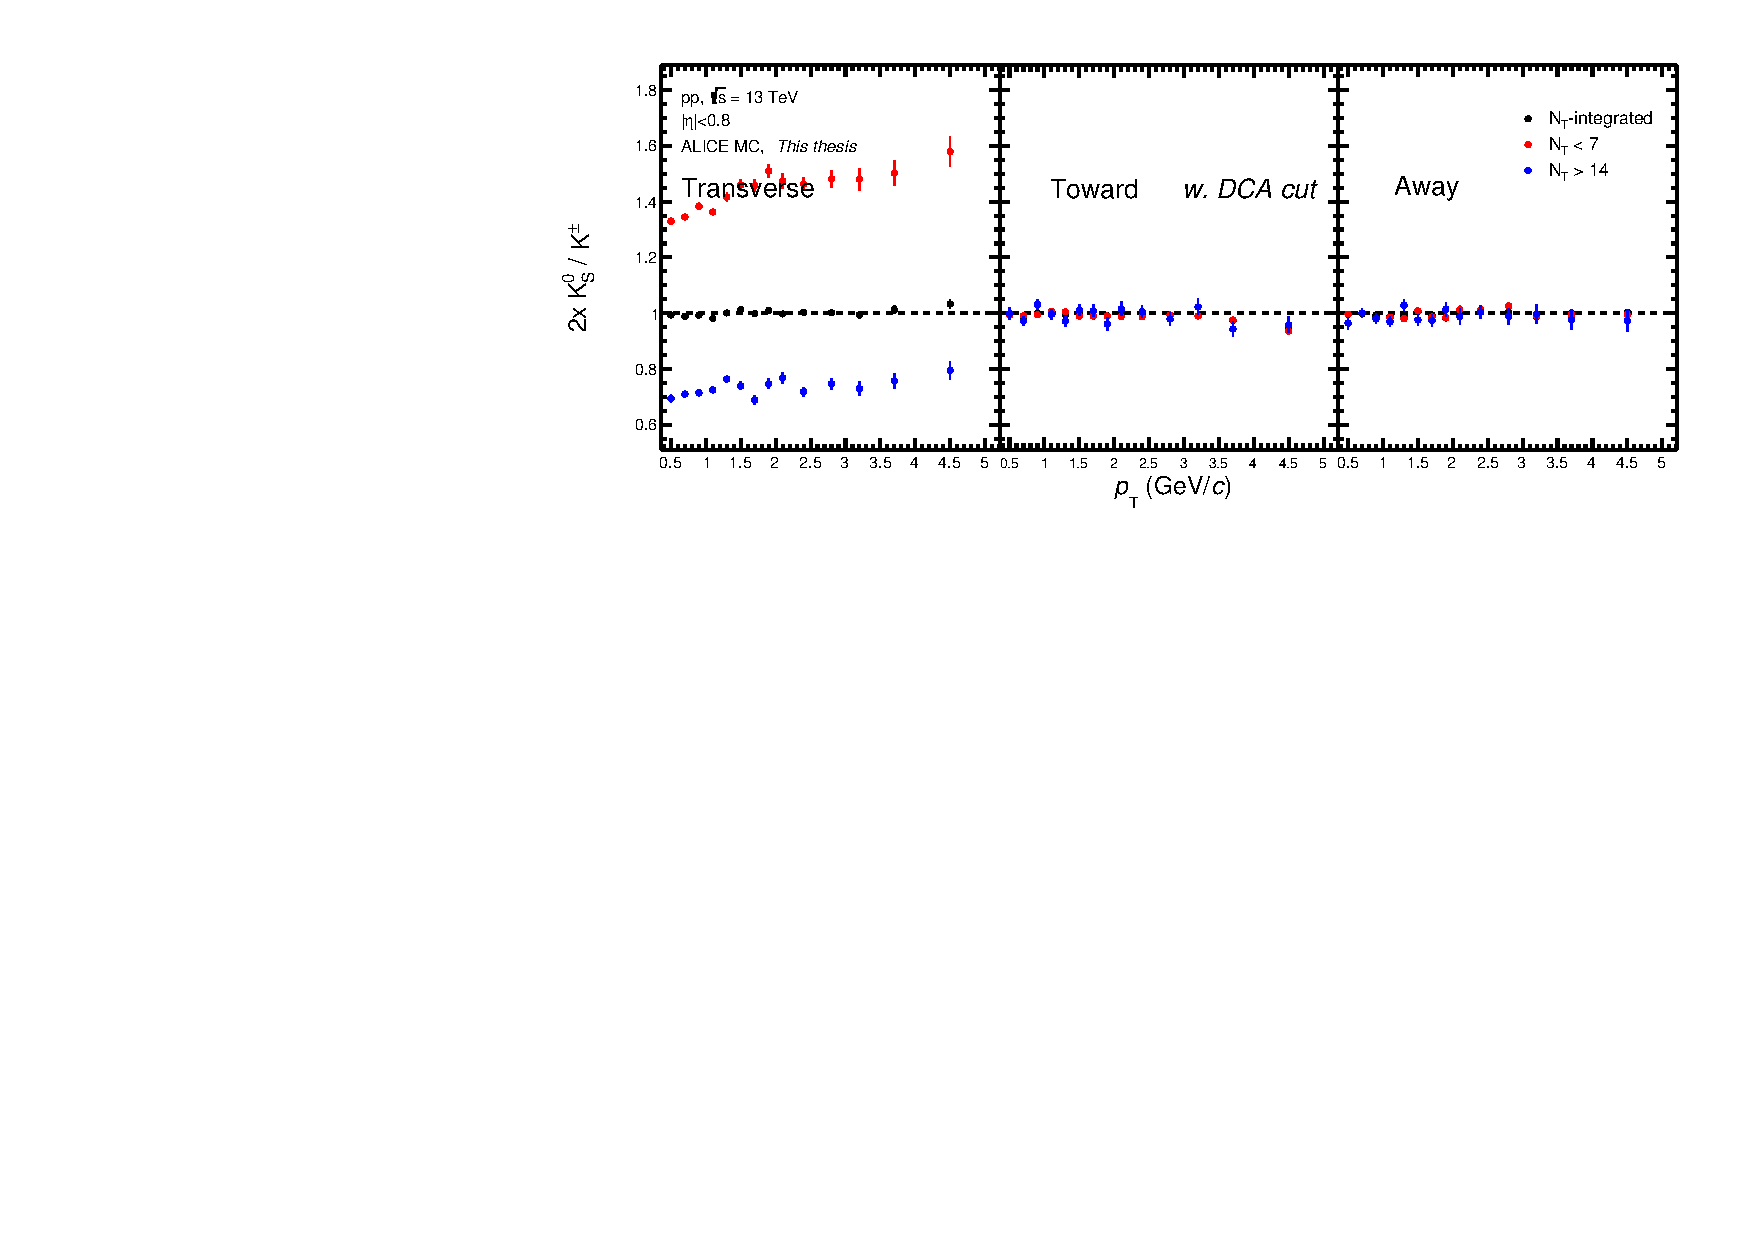
\includegraphics[width=.990\textwidth]{\imgpath/KtoK_new.pdf}}\\
\caption{Transverse momentum spectra ratios of the neutral \KOs to the charged \kpm without enforcing the DCA cute (top) and after its inclusion (bottom) in the three azimuthal regions. Events with low \NT (red) and high \NT (blue) are compared. The results come from ALICE detector simulations, are uncorrected for reconstruction effects and acceptance, and show only statistical uncertainties.}
\label{fig:rt:KtoK}
\end{figure}



\section{Bayesian unfolding procedure}

The measurements of \VOs are conducted as a function of the number of measured tracks \NTm within the detector acceptance. The measured multiplicity \NTm includes a fraction of the true primary charged-particle multiplicity \NTt not lost due to acceptance, efficiency, or track selection, as well as contributions from secondary particles or particles smeared into the measurement's kinematic acceptance due to detector resolution (i.e., from $\pt < \gevc{0.15}$). These effects fluctuate on an event-by-event basis and thus there is no unique correlation between \NTm and \NTt. This means that events with true multiplicity \NTt can be measured with different \NTm, contributing to \VO measurements in multiple \NTm bins. Therefore, each spectrum contains particles from events with many true multiplicities \NTt.

This thesis uses a Bayesian unfolding procedure, as discussed in Ref.~\cite{dagostiniMultidimensionalUnfoldingMethod1995}, to convert \VOs measurements as a function of \NTm into measurements as a function of \NTt and thus correct for the mentioned effects.

\subsection{One-dimensional unfolding}

The measured multiplicity distribution $\nev(\NTm)$ can be mathematically represented as the result of convolving (or ``folding") the true multiplicity distribution produced by the collisions, $\nev(\NTt)$, with the detector's response function. The response matrix $\mathrm{S}_{mt}$, which represents the conditional probability $P(\NTm | \NTt)$ of an event with multiplicity \NTt being measured with multiplicity \NTm, can be obtained from MC simulations of the apparatus. Using this matrix, also shown in Fig.~\ref{fig:rt:matrix}, $\nev(\NTm)$ can be expressed in terms of $\nev(\NTt)$ as follows:
\begin{align}
\nev(\NTm) = \sum_t \mathrm{S}_{mt} \cdot \nev(\NTt) \quad ,
\end{align}
To obtain the true multiplicity distribution from the measured distribution, the inverse of $S_{mt}$ could be used, hypothetically, as shown below:
\begin{align}
\nev ( \NTt ) = \sum_m \mathrm{S}_{mt}^{-1} \cdot \nev ( \NTm ) \quad .
\end{align}
However, the inverse $\mathrm{S}_{mt}^{-1}$ may have multiple or zero solutions, making this approach unfeasible. Alternatively, $\mathrm{S}_{mt}^{-1}$ could be obtained directly from MC simulations, just like the detector response. However, this matrix would then strongly depend on the generated \NTt distribution and be significantly model-dependent, as physics generators vary in their \NTt predictions. In contrast, the detector response is mostly affected by the accuracy of the particle propagation simulations, which is a lot better understood. Therefore, an iterative numerical procedure based on Bayes' theorem is used to obtain the unfolding matrix $\mathrm{M}_{mt}$, which represents the conditional probabilities $P(\NTt | \NTm)$ \cite{dagostiniMultidimensionalUnfoldingMethod1995}.

In this application, Bayes' theorem can be expressed in terms of \NTm and \NTt as follows,
\begin{align}
\label{eq:rt:bayes}
P(\NTt | \NTm) = \dfrac{P(\NTm | \NTt)P(\NTt)}{P(\NTm)} \quad ,
\end{align}
where $P(\NTt)$ and $P(\NTm)$ are probability distributions for an event occurrence with \NTt and \NTm, respectively. Assuming that $P(\NTt)$ is known, $P(\NTm)$ can be calculated as follows:
\begin{align}
P(\NTm) = \sum_t P(\NTm | \NTt) P(\NTt) \quad .
\end{align}
Therefore, using Eq.~\ref{eq:rt:bayes}, the conditional probability in the unfolding matrix can be written as follows:
\begin{align}
P(\NTt | \NTm) = \dfrac{P(\NTm | \NTt)P(\NTt)}{\sum_{t'} P(\NTm | \NTtt) P(\NTtt)} \quad .
\end{align}

However, $P(\NTt)$ (the ``prior") is initially unknown and must be arbitrarily chosen. The unfolding matrix can be calculated using this prior, and the unfolded distribution can be obtained as follows:
\begin{align}
\nevhat(\NTt) = \sum_m P(\NTt | \NTm) \nev(\NTm) \quad .
\end{align}
This unfolded multiplicity can subsequently be used to update the prior as follows:
\begin{align}
\hat{P}(\NTt) = \dfrac{\nevhat(\NTt)}{\sum_{t'} \nevhat(\NTtt)} \quad ,
\end{align}
starting a new iteration. The updated $\hat{P}(\NTt)$ is closer to the true $P(\NTt)$ than the initial guess because the arbitrarily chosen prior is constrained by the $\nev(\NTm)$ observable, which contains information about $P(\NTt)$. The statistical uncertainties are propagated according to the discussion in Ref.~\cite{dagostiniMultidimensionalUnfoldingMethod1995}.

Multiple approaches can be taken to choose the prior: a uniform distribution, the $\NTt$ distribution generated by a model, or the $\NTm$ distribution acquired from data. In this thesis, the prior choice was found to not play a role and the $\NTm$ distribution was used.

The $\chi^2/\mathrm{ndf}$ is calculated to determine the validity of the correction and the stopping point for the iterative process. It is calculated by comparing the $\NTt$ distribution -- known a priori in the simulations -- and the unfolded $\nevhat(\NTt)$ distribution, where $\mathrm{ndf}$ refers to the number of degrees of freedom, in this case the number of data points in the distribution. The process is stopped when $\chi^2/\mathrm{ndf}$ reaches a minimum value or the iterations take a maximum number of steps $n_\mathrm{iter}$. This is imposed to avoid overfitting and overestimation of statistical uncertainties. 

In this dissertation, the $\NTmin$ and $\NTmax$ distributions are unfolded analogously to the $\NT$ case. The selected $n_\mathrm{iter}$ values are reported in Tab.~\ref{tab:rt:niter}. The entire iterative process is summarised in a diagram shown in Fig.~\ref{fig:rt:bayes}. 

\begin{figure}%
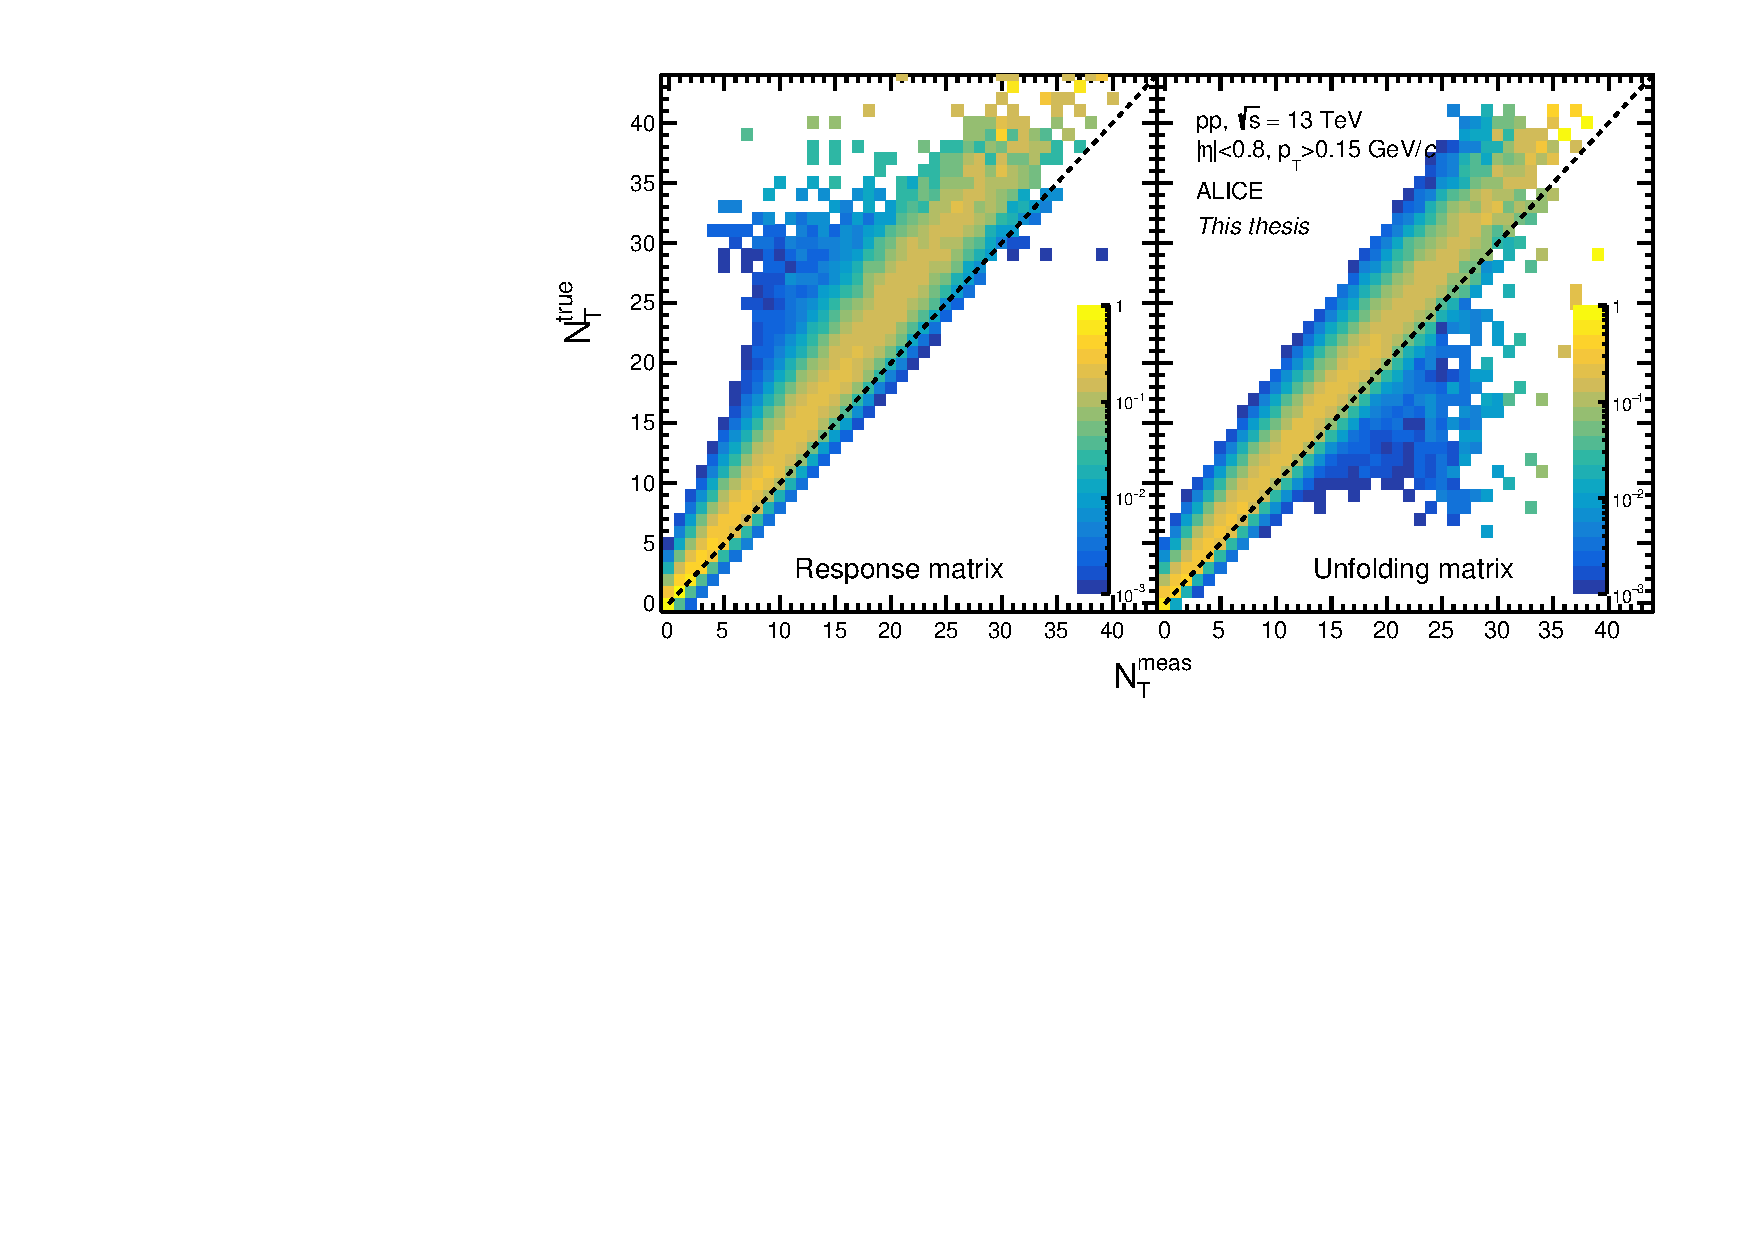
\includegraphics[width=.990\textwidth]{\imgpath/InfoRT_matrix.pdf}\\
\caption{\textbf{(left)} Response matrix $\mathrm{S}_{mt}$ showing the correlation between measured and true track multiplicity in the Transverse region determined from ALICE MC simulations based on Pythia 8. The matrix is row-wise normalised. \textbf{(right)} Unfolding matrix $P(\NTt | \NTm)$ calculated from the iterative Bayesian unfolding procedure.}
\label{fig:rt:matrix}
\end{figure}

The used response matrix, as well as the resulting unfolding matrix, can be seen in Fig.~\ref{fig:rt:matrix}. The method still exhibits some degree of model dependence due to the generation of the response matrix. Previous studies in ALICE have compared the response matrix for \NT acquired from Pythia 8 and from EPOS LHC MC simulations, which revealed that the effect is less than $1\%$ \cite{vazquezruedaStudyProductionPp2022}. This effect is taken into consideration as a source of systematic uncertainty.

\begin{table}[h!]
\centering
\caption{The number of iterations in the Bayesian unfolding process for \NT (capped at maximum $n_\mathrm{iter}$), \NTmin, and \NTmax.}
\label{tab:rt:niter}
\begin{tabular}{|cc|ccc|}
\hline
\multicolumn{2}{|r|}{\parbox[b][1.2em]{2em}{} Unfolding observable} & \NT & \NTmin & \NTmax \\ \hline
\multicolumn{2}{|c|}{\parbox[b][1.1em]{1em}{}$n_\mathrm{iter}$} & $20$ (max.) & $10$ & $18$ \\ \hline
\end{tabular}
\end{table}


\begin{figure}[h]
		\centering
		\begin{tikzpicture}[node distance=0.8cm,box/.style={draw, rounded corners=.2cm}]
			%\node[box, text width=0.9\textwidth, align=center] (eqn) {\NTt ...\ true multiplicity};
			%below=of eqn
			\node[box, fill=black!10, text width=0.9\textwidth, align=center] (thm) {Bayes' Theorem\\\vspace{1em}$P(\NTt | \NTm) = \dfrac{P(\NTm | \NTt)P(\NTt)}{P(\NTm)}$};
			\node[box, below=of thm, align=center] (f1) {Unfolding matrix\\
			\\$P(\NTt | \NTm) = \dfrac{P(\NTm | \NTt)P(\NTt)}{\sum_{t'}P(\NTm | \NTtt)P(\NTtt)}$};
			\node[draw=none, below=of f1, align=center] (f2) {\begin{Large}$\times \, n_\mathrm{iter}$\end{Large}};
			\node[draw=none, below=of f2, align=center] (f0) {};
			\node[box, left=of f0, text width=.47\textwidth,text height=1em, align=center] (f3) {Unfolded distribution\\\vspace{1em}$\nevhat(\NTt) = \sum_m P(\NTt | \NTm) \nev(\NTm)$};
			\node[box, right=of f0, text width=.40\textwidth, text height=1em, align=center] (f4) {Updated prior\\\vspace{0.5em}$\hat{P}(\NTt) = \dfrac{\nevhat(\NTt)}{\sum_{t'} \nevhat(\NTtt)}$};
			\draw[-{Latex[bend]}, ultra thick, blue] (f1) to[bend right=50] (f3);
			\draw[-{Latex[bend]},ultra thick, blue] (f3) to[bend right] (f4);
			\draw[-{Latex[bend]},ultra thick, blue] (f4) to[bend right=50] (f1);
		\end{tikzpicture}
		\caption{Diagram showing the iterative process of Bayesian unfolding.}
		\label{fig:rt:bayes}
\end{figure}


\subsection{Unfolding of \KOs, \LA, and \AL \pt spectra}

In the unfolding treatment of the \LA and \AL, the particle and the anti-particle \pt spectra were combined to reduce statistical uncertainties and increase the method's robustness. For the Toward and Away regions, the spectra can be unfolded in a similar fashion to the \NT activity, assuming that they are completely decoupled from the production in the Transverse region. This implies mere reshuffling of \VOs in individual \pt bins $n^{\VO}_{\pt=i}$ between different events, based on the unfolding recipe established above:
\begin{align}
\hat{n}^{\VO}_{\pt=i}(\NTt) = \sum_m P(\NTt | \NTm) n^{\VO}_{\pt=i}(\NTm) \quad .
\end{align} 

Closure tests using MC simulations were conducted to compare the unfolded \pt spectra as a function of unfolded-reconstructed \NT to the generated \pt spectra as a function of generated \NT -- and showed the plausibility of this approach. The closure tests are presented in Fig.~\ref{fig:rt:closures}, indicating mostly consistent results within $5\%$, with the deviations observed more in the \RT extremes.

For the treatment of the Transverse regions, two approaches were considered:
\begin{enumerate}
\item Similarly to how this unfolding method was applied in other multiplicity and \NT measurements in ALICE for charged particles \cite{vazquezruedaStudyProductionPp2022}, one assumes correlations between the \pt spectra and the event activity. This approach requires multiplying the response matrix with number of tracks in each column, modifying the unfolding matrix to make it \pt-dependent, and applying different unfolding recipes to \VOs based on their \pt, which approximates reshuffling on a particle-by-particle basis.
\item Given the fact that the \NT tracks and the \VO daughters were made two disjunct sets in this measurement by separating them with a $|\mathrm{DCA}_{xy}|$ boundary, one may assume complete de-correlation between the \VO \pt spectra and the measured \NT. Subsequently, the Transverse region would be treated like the Toward and Away.
\end{enumerate}

In this study, both approaches were tested and the second method was chosen for the measurement. Although the first method generally produced somewhat smaller non-closure discrepancies, the second method is more logically sound. Additionally, modifying the response matrix in the first method resulted in an empty zeroth bin by construction. As a consequence, events with $\NT = 0$ but the number of \VOs $n^{\VO}>0$ could not be treated since the unfolding matrix cannot recover this scenario. While this is not a limitation in charged particle analyses since such cases cannot occur, it posed a problem here.

The closure tests for the Transverse region are shown in Fig.~\ref{fig:rt:closures}, but it should be noted that they exhibit somewhat larger deviations (up to $10\%$) in the most extreme bins of \RT compared to the Toward/Away regions. One possible explanation for this is the simplicity of the unfolding method used here, as well as the fact that the closure tests were conducted on Pythia simulations, which due to the local string breakings may exhibit strongly correlated particle production in phase space, leading to somewhat of a coupling between \NT and \VOs.

Unfolding of the \VOs spectra in the Transverse-min and Transverse-max regions as a function of \NTmin and \NTmax, respectively, was performed in an identical manner. Although the results close well in MC tests in the central \RTmin/\RTmax intervals, deviations of up to around $20\%$ are observed in the most extreme bins, as depicted in Fig.~\ref{fig:rt:closures}. This is likely due to low statistics samples, the simplicity of the method, and the fact that the individual \RTmin/\RTmax intervals cover even smaller ranges of \NTmin/\NTmax, making the process highly sensitive to fluctuations.

\begin{figure}[H]%
\def \PID {K0s}
\subfloat[][]{\includegraphics[width=.24\textwidth]{\imgpath/Toward_PID_\PID_RT_1.pdf}\includegraphics[width=.24\textwidth]{\imgpath/Trans1D_PID_\PID_RT_1.pdf}\includegraphics[width=.24\textwidth]{\imgpath/TransMin1D_PID_\PID_RT_1.pdf}\includegraphics[width=.24\textwidth]{\imgpath/TransMax1D_PID_\PID_RT_1.pdf}}\\
\subfloat[][]{\includegraphics[width=.24\textwidth]{\imgpath/Toward_PID_\PID_RT_3.pdf}\includegraphics[width=.24\textwidth]{\imgpath/Trans1D_PID_\PID_RT_3.pdf}\includegraphics[width=.24\textwidth]{\imgpath/TransMin1D_PID_\PID_RT_3.pdf}\includegraphics[width=.24\textwidth]{\imgpath/TransMax1D_PID_\PID_RT_3.pdf}}\\
\def \PID {L}%
\subfloat[][]{\includegraphics[width=.24\textwidth]{\imgpath/Toward_PID_\PID_RT_1.pdf}\includegraphics[width=.24\textwidth]{\imgpath/Trans1D_PID_\PID_RT_1.pdf}\includegraphics[width=.24\textwidth]{\imgpath/TransMin1D_PID_\PID_RT_1.pdf}\includegraphics[width=.24\textwidth]{\imgpath/TransMax1D_PID_\PID_RT_1.pdf}}\\
\subfloat[][]{\includegraphics[width=.24\textwidth]{\imgpath/Toward_PID_\PID_RT_3.pdf}\includegraphics[width=.24\textwidth]{\imgpath/Trans1D_PID_\PID_RT_3.pdf}\includegraphics[width=.24\textwidth]{\imgpath/TransMin1D_PID_\PID_RT_3.pdf}\includegraphics[width=.24\textwidth]{\imgpath/TransMax1D_PID_\PID_RT_3.pdf}}
\caption{Transverse momentum Monte Carlo closure tests between true spectra and reconstructed, corrected, and unfolded spectra for \textbf{(a)} \KOs low-\RT/\RTmin/\RTmax events, \textbf{(b)} \KOs high-\RT/\RTmin/\RTmax events, \textbf{(c)} \LA+\AL low-\RT/\RTmin/\RTmax events, and \textbf{(d)} \LA+\AL high-\RT/\RTmin/\RTmax events. The columns show the regions in this order: Toward, Transverse, Transverse-min, and Transverse-max. A $10\%$-effect band is indicated.}
\label{fig:rt:closures}
\end{figure}


\section{\RT, \RTmin, \RTmax distributions}

The unfolded \NT, \NTmin, and \NTmax distributions were self-normalised to obtain the \RT, \RTmin, and \RTmax distributions, respectively. The mean values used for self-normalisation are reported in Tab.~\ref{tab:rt:meannt}. They are shown in Fig.~\ref{fig:rt:rtdistr} and compared with predictions from Pythia 8 (Monash tune \cite{skandsTuningPYTHIAMonash2014} and Ropes tune \cite{bierlichEffectsOverlappingStrings2015}) as well as EPOS LHC \cite{pierogEPOSLHCTest2015}. 

\begin{table}[h!]
\centering
\caption{Mean number of transverse multiplicities used in the definition of \RT, \RTmin, and \RTmax.}
\label{tab:rt:meannt}
\begin{tabular}{|cc|ccc|}
\hline
\multicolumn{2}{|r|}{\parbox[b][1.2em]{2em}{} Event classifier} & \RT & \RTmin & \RTmax \\ \hline
\multicolumn{2}{|c|}{\parbox[b][1.1em]{1em}{} Average \NT/\NTmin/\NTmax} & $7.345$ & $2.470$ & $4.869$ \\ \hline
\end{tabular}
\end{table}

The results can be described by the predictions quite accurately, favouring EPOS LHC, but show deviations in high-UE-activity events. The different quantiles corresponding to the $\RT/\RTmin/\RTmax$ ranges used in this measurement are highlighted. They are also summarised in Tab.~\ref{tab:rt:rtbins}. It should be noted that since the transverse multiplicities are non-negative integers, $\NT, \NTmin, \NTmax \in \mathbb{N}_0$, the $\RT/\RTmin/\RTmax$ distributions are not continuous observables.

\begin{figure}[H]%
\subfloat[][]{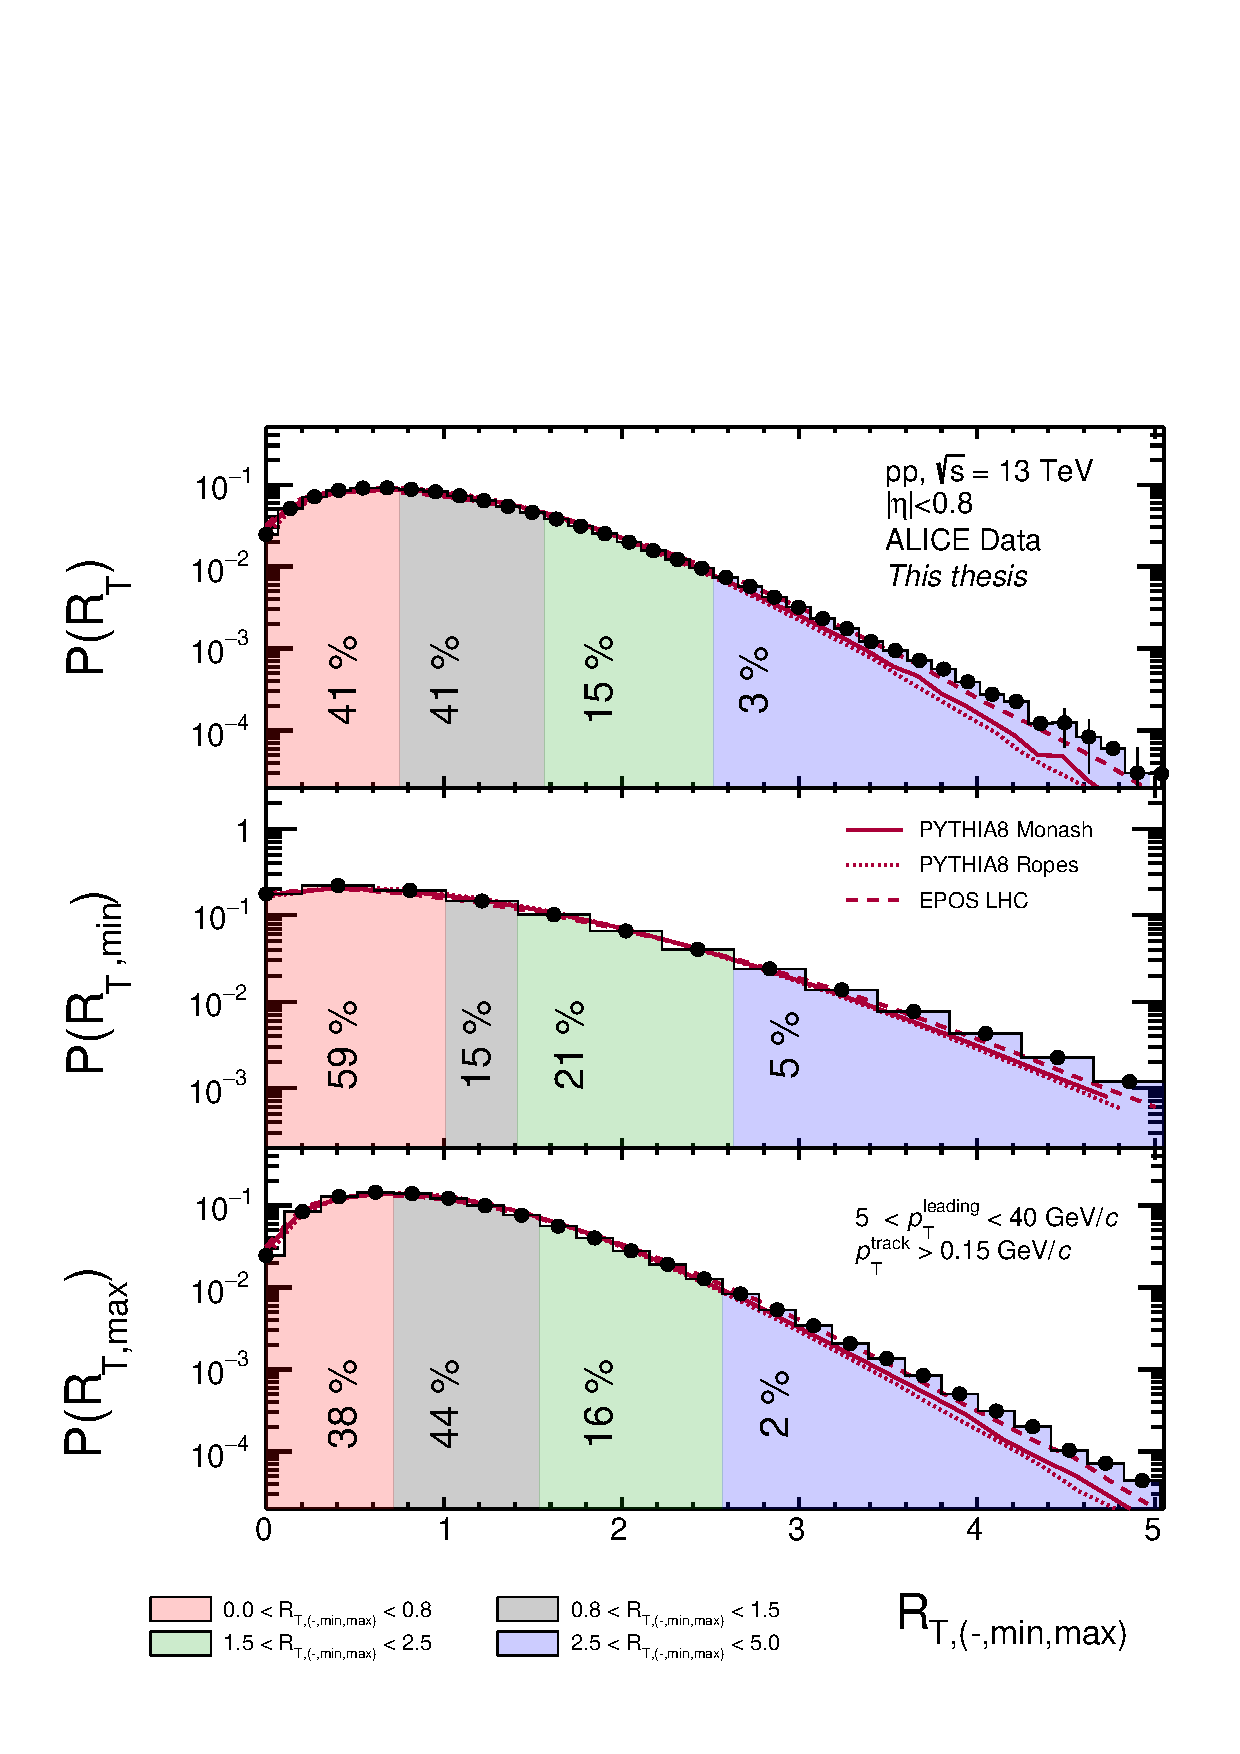
\includegraphics[width=.990\textwidth]{\imgpath/Rt_distr.pdf}}\\
\caption{Probability distribution function of the underlying event activity classifiers \RT (top), \RTmin (middle), and \RTmax (bottom) in pp collisions at \sppt{13} in events with a high-\pt track $5 < \pt < \gevc{40}$. The results are treated with Bayesian unfolding and compared with predictions from Pythia 8 Monash, Pythia 8 Ropes, and EPOS LHC. The \RT/\RTmin/\RTmax intervals used in this dissertation are shown along with the corresponding quantile values. Only statistical uncertainties are shown.}
\label{fig:rt:rtdistr}
\end{figure}

\begin{table}
\centering
\caption{The intervals for UE activity classifier selected in this measurement and the corresponding average values.}
\label{tab:rt:rtbins}
\begin{tabular}{|cc|ccc|}
\hline
\multicolumn{2}{|r|}{\parbox[b][1.2em]{2em}{} Average values} & $\langle \RT \rangle$ & $\langle \RTmin \rangle$ & $\langle \RTmax \rangle$ \\ \hline
%\multicolumn{2}{l|}{} & \multicolumn{3}{l}{} \\
\multicolumn{5}{l}{\parbox[b][1.4em]{1em}{Intervals}} \\ \hline
\multicolumn{2}{|l|}{\parbox[b][1.1em]{1em}{}0--0.85} & $0.49$ & $0.42$ & $0.53$ \\
\multicolumn{2}{|l|}{\parbox[b][1.1em]{1em}{}0.85--1.5} & $1.19$ & $1.21$ & $1.20$ \\
\multicolumn{2}{|l|}{\parbox[b][1.1em]{1em}{}1.5--2.5} & $1.92$ & $1.90$ & $1.91$ \\
\multicolumn{2}{|l|}{\parbox[b][1.1em]{1em}{}2.5--5.0} & $2.97$ & $3.27$ & $3.01$ \\ \hline
\end{tabular}
\end{table}

\section{Systematic uncertainties}

The systematic uncertainties on the \pt spectra were determined individually for each \RT interval and azimuthal region, following the procedures described in Section~\ref{sec:ana:syst}. They are reported in Fig.~\ref{fig:rt:systK0s}, Fig.~\ref{fig:rt:systLA}, and Fig.~\ref{fig:rt:systAL} for the \KOs, \LA, and \AL, respectively. Furthermore, they are summarised in Tab.~\ref{tab:rt:syst}. The dominant contributions to systematic uncertainties, in no specific order, come from signal extraction, selection cuts related to TPC tracking and topological reconstruction, and the requirement of signals from fast detectors to reject track pile-up.

As there are no reasons to believe the systematic uncertainties should differ when using the more specific UE activity classifiersin the two Transverse sub-regions, they are subsequently also applied in the \RTmin and \RTmax measurements.

\textit{Make the style consistent with the spherocity chapter.}

\begin{figure}[H]%
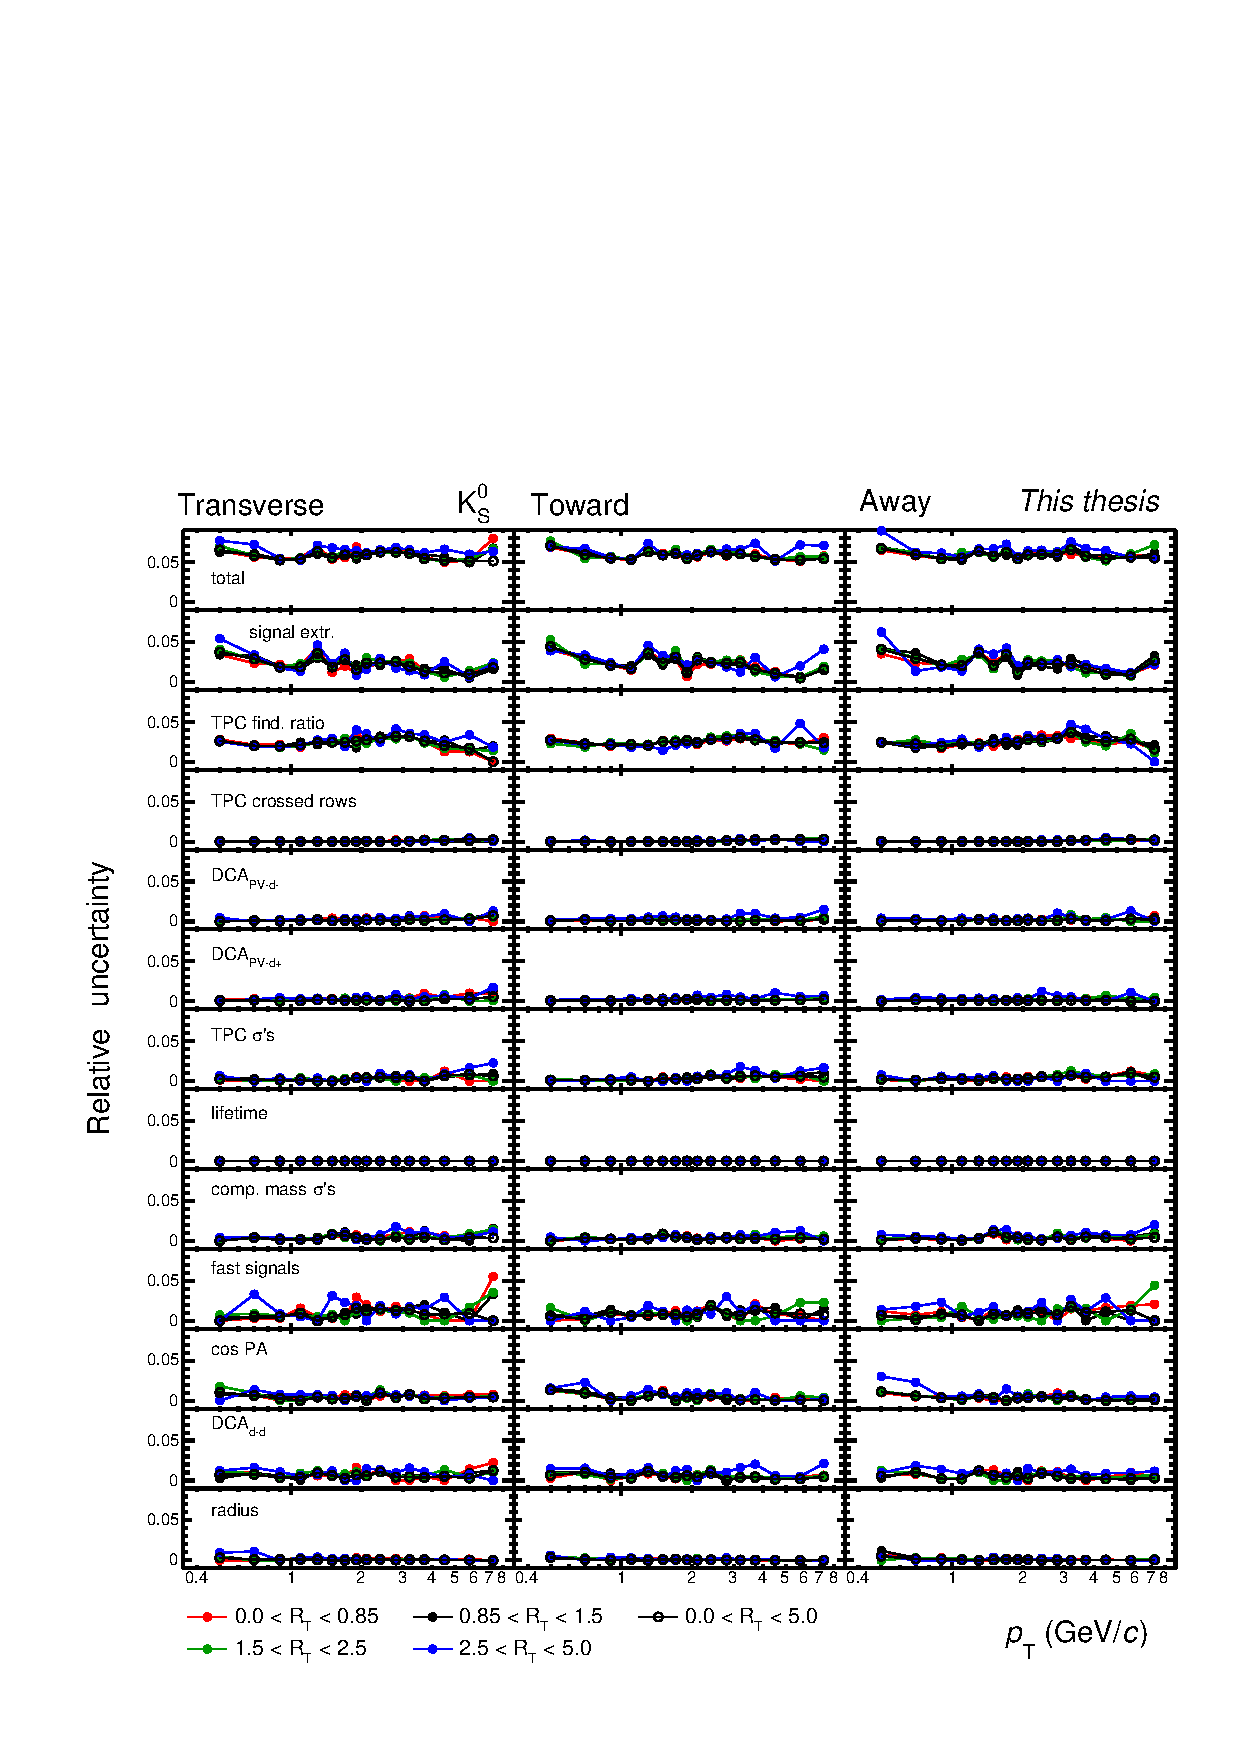
\includegraphics[width=.990\textwidth]{\imgpath/InfoRT_syst_K0s.pdf}\\
\caption{Summary of the relative systematic uncertainties on transverse momentum spectra and the individual contributions for \KOs in the \textbf{(left)} Transverse, \textbf{(middle)} Toward, and \textbf{(right)} Away in the different \RT intervals.}
\label{fig:rt:systK0s}
\end{figure}

\begin{figure}[H]%
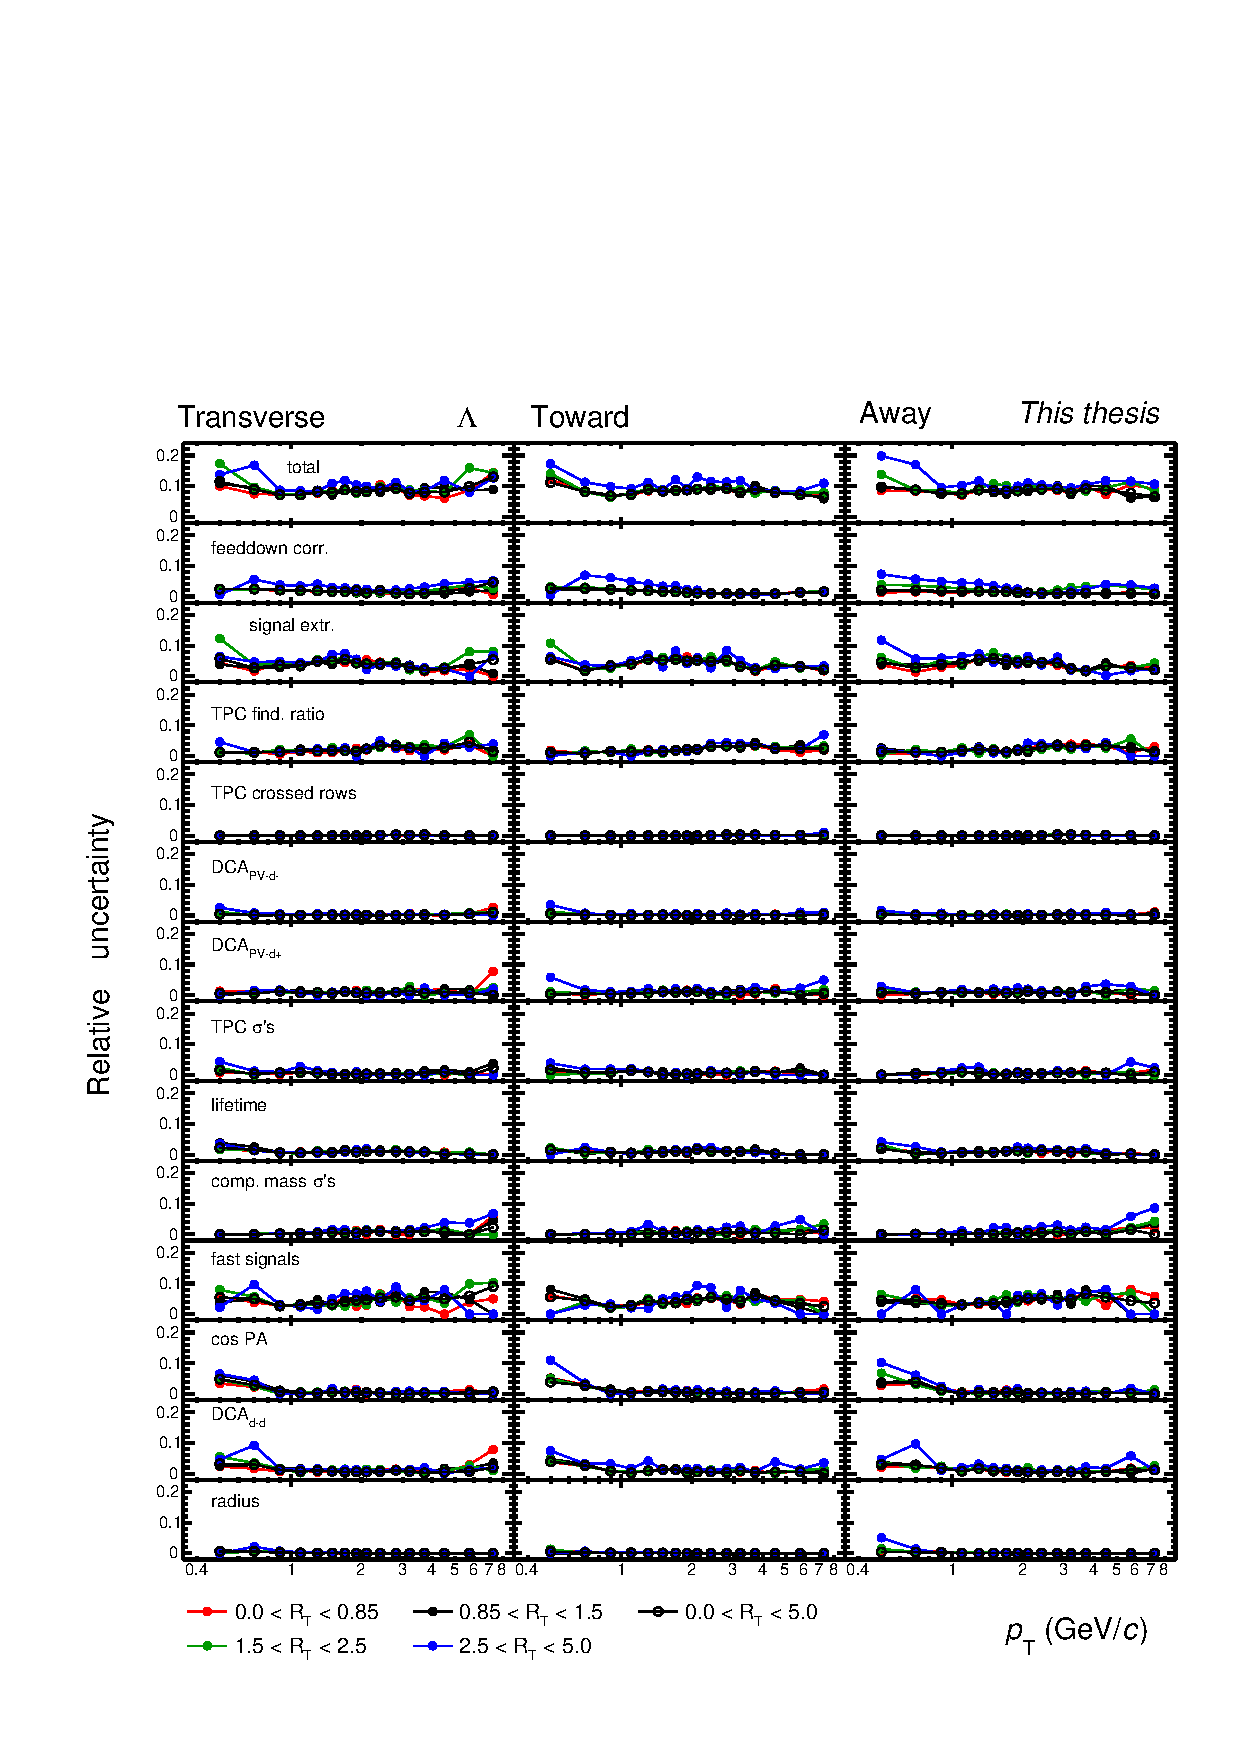
\includegraphics[width=.990\textwidth]{\imgpath/InfoRT_syst_L.pdf}\\
\caption{Summary of the relative systematic uncertainties on transverse momentum spectra and the individual contributions for \LA in the \textbf{(left)} Transverse, \textbf{(middle)} Toward, and \textbf{(right)} Away in the different \RT intervals.}
\label{fig:rt:systLA}
\end{figure}

\begin{figure}[H]%
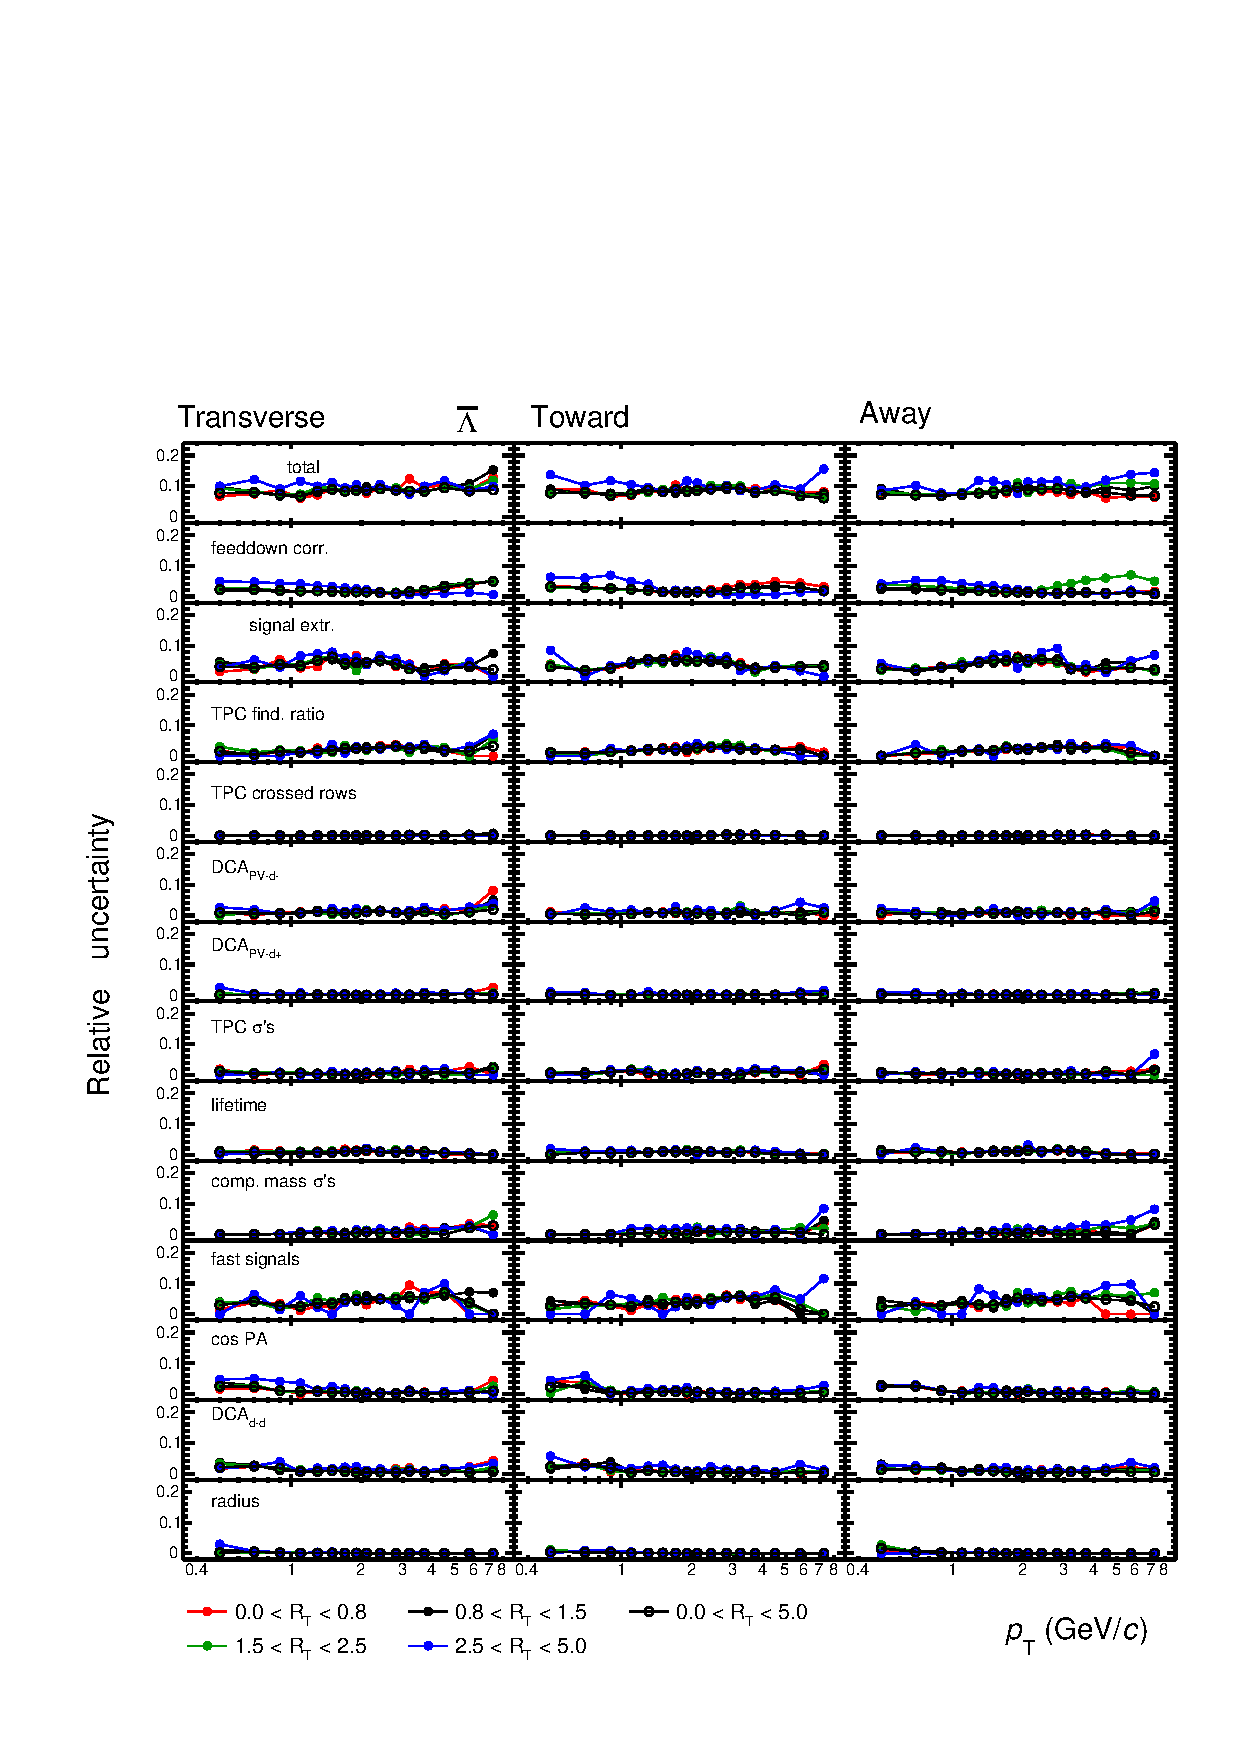
\includegraphics[width=.990\textwidth]{\imgpath/InfoRT_syst_Lbar.pdf}\\
\caption{Summary of the relative systematic uncertainties on transverse momentum spectra and the individual contributions for \AL in the \textbf{(left)} Transverse, \textbf{(middle)} Toward, and \textbf{(right)} Away in the different \RT intervals.}
\label{fig:rt:systAL}
\end{figure}

\subsection{Uncertainties from the unfolding procedure}

The deviations between the generated \pt spectra and the reconstructed, corrected, and unfolded \pt spectra displayed in Fig.~\ref{fig:rt:closures} were used to determine the systematic uncertainties associated with the unfolding procedure. To isolate the effect of unfolding from other reconstruction effects, the ``non-closures" in each $\RT/\RTmin/\RTmax$ interval were divided by the non-closure in the $\RT/\RTmin/\RTmax$-integrated bin.

The unfolding systematic uncertainties exhibited a large amount of correlation between \KOs and \LA. This correlation was expected, as the \VO species should unfold in similar patterns. Therefore, the systematic uncertainty on the baryon-to-meson ratio was also calculated independently to avoid these correlations and reduce the systematic uncertainty on those results.

Moreover, in the most extreme bins, the non-closures sometimes exhibited unrealistic deviations from unity due to limited statistics and fluctuations. To address this issue, a smoothing procedure was applied by fitting the resulting uncertainties with first- and second-order polynomials. The results are shown in Fig.~\ref{fig:rt:systUnf}.

\begin{figure}[H]%
\subfloat[][]{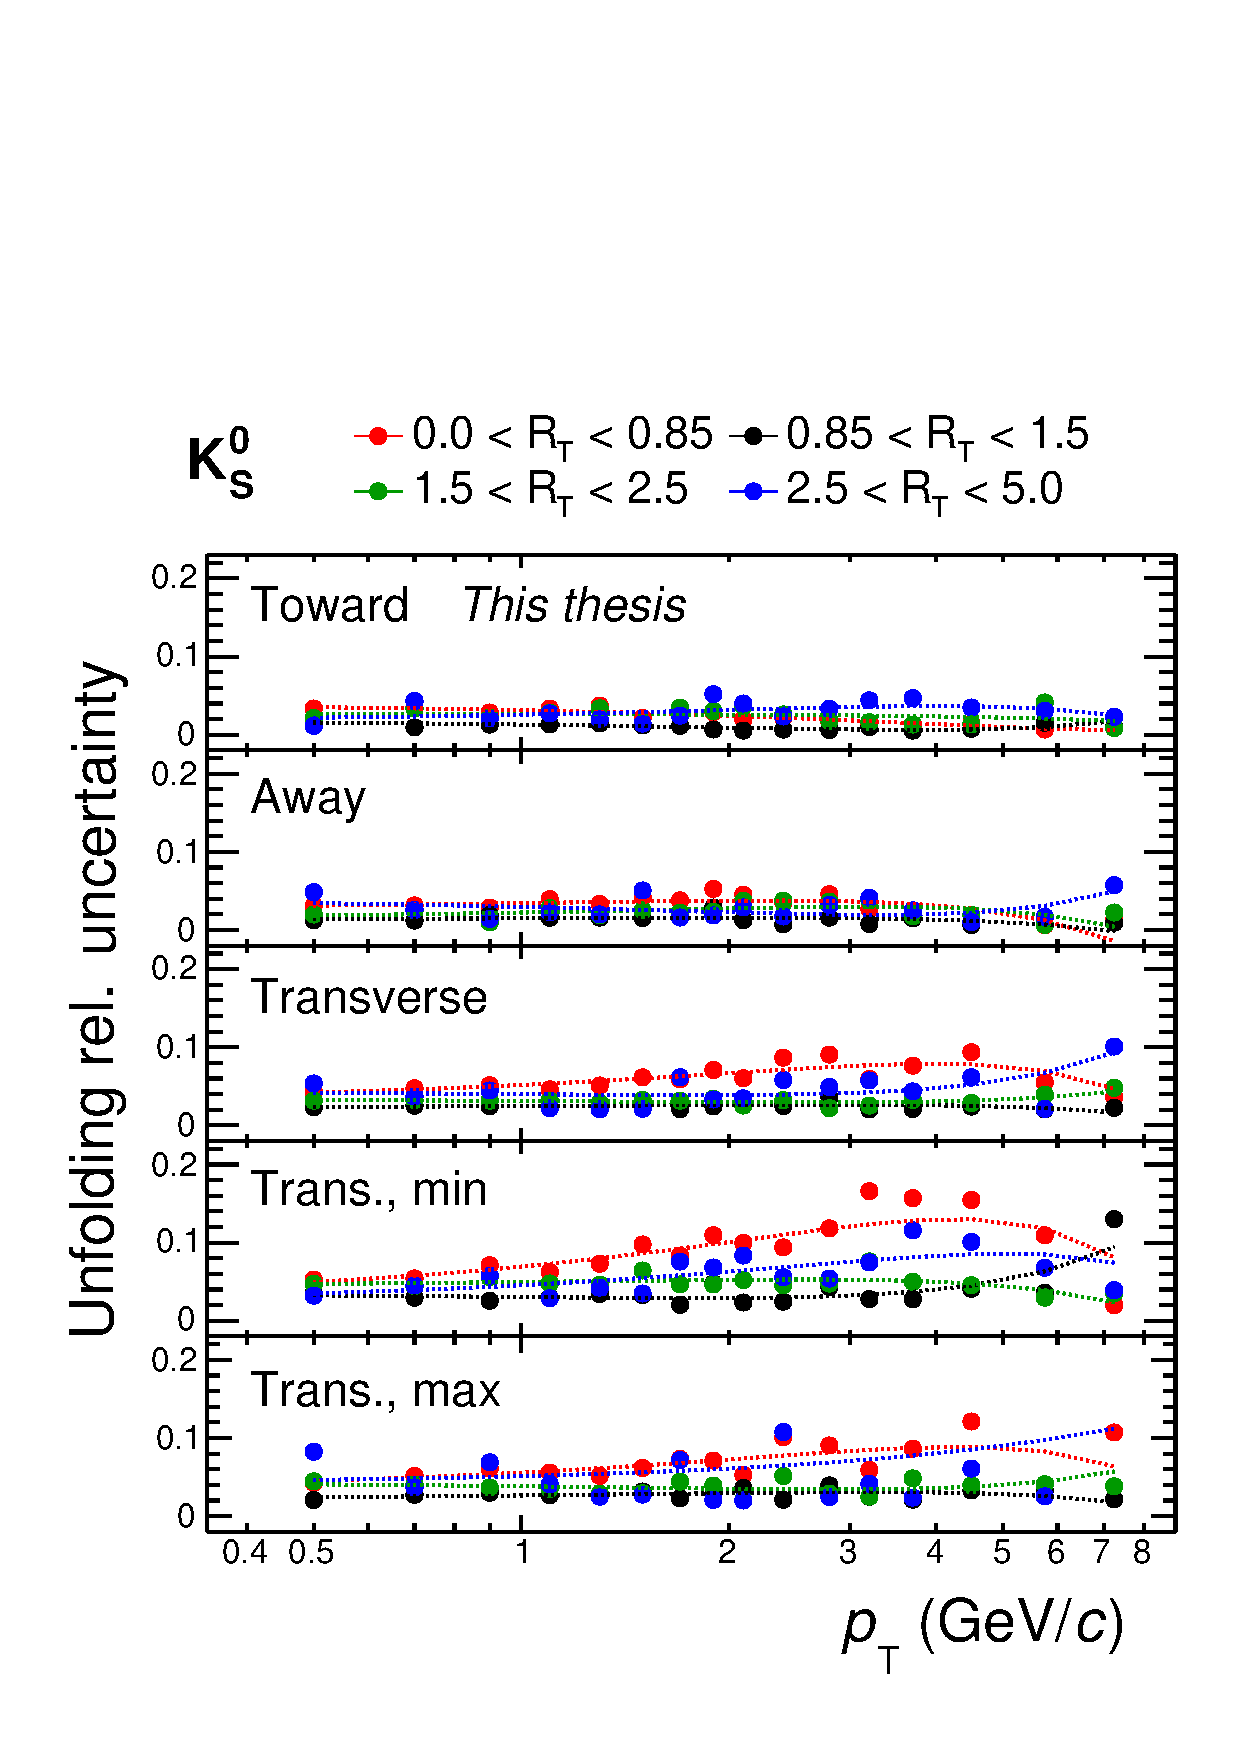
\includegraphics[width=.320\textwidth]{\imgpath/InfoRT_systUnf_K0s.pdf}}
\subfloat[][]{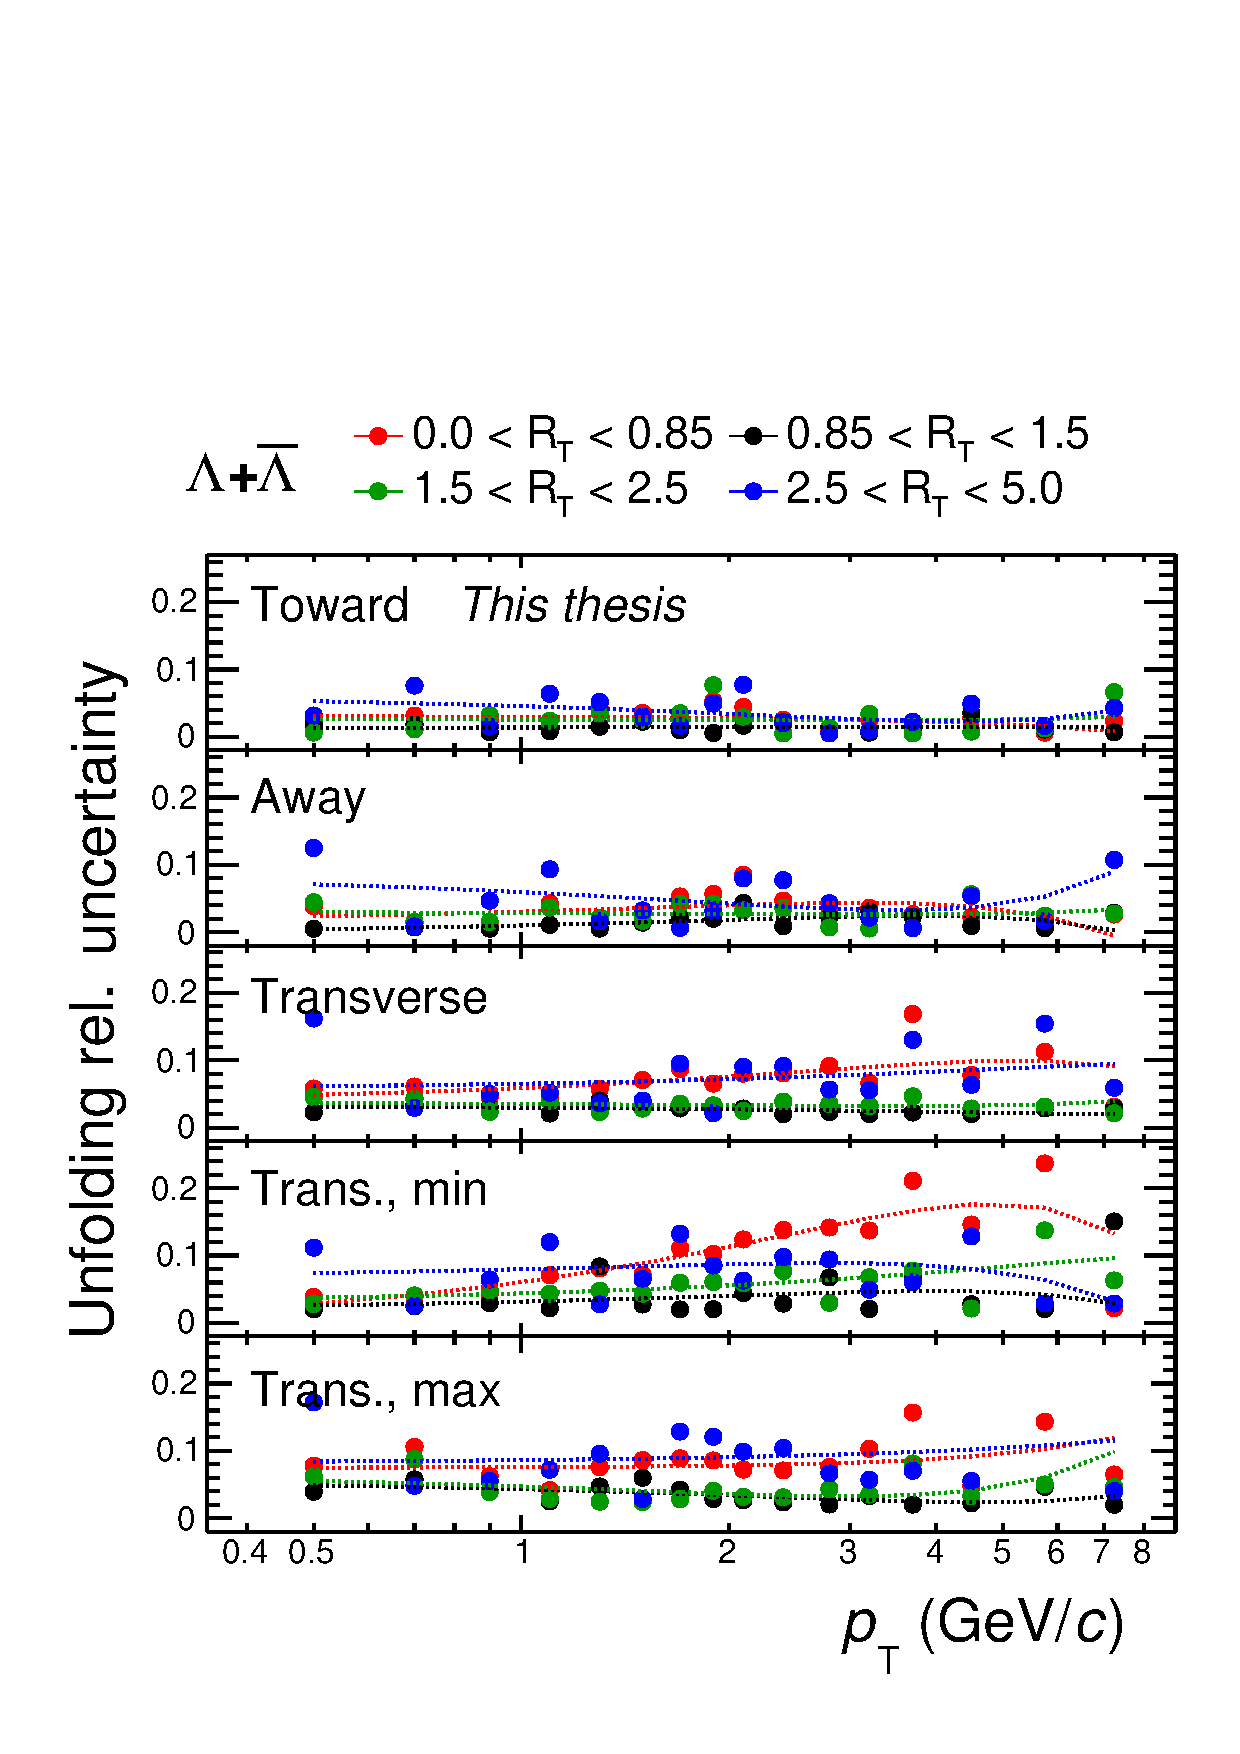
\includegraphics[width=.320\textwidth]{\imgpath/InfoRT_systUnf_L.pdf}}
\subfloat[][]{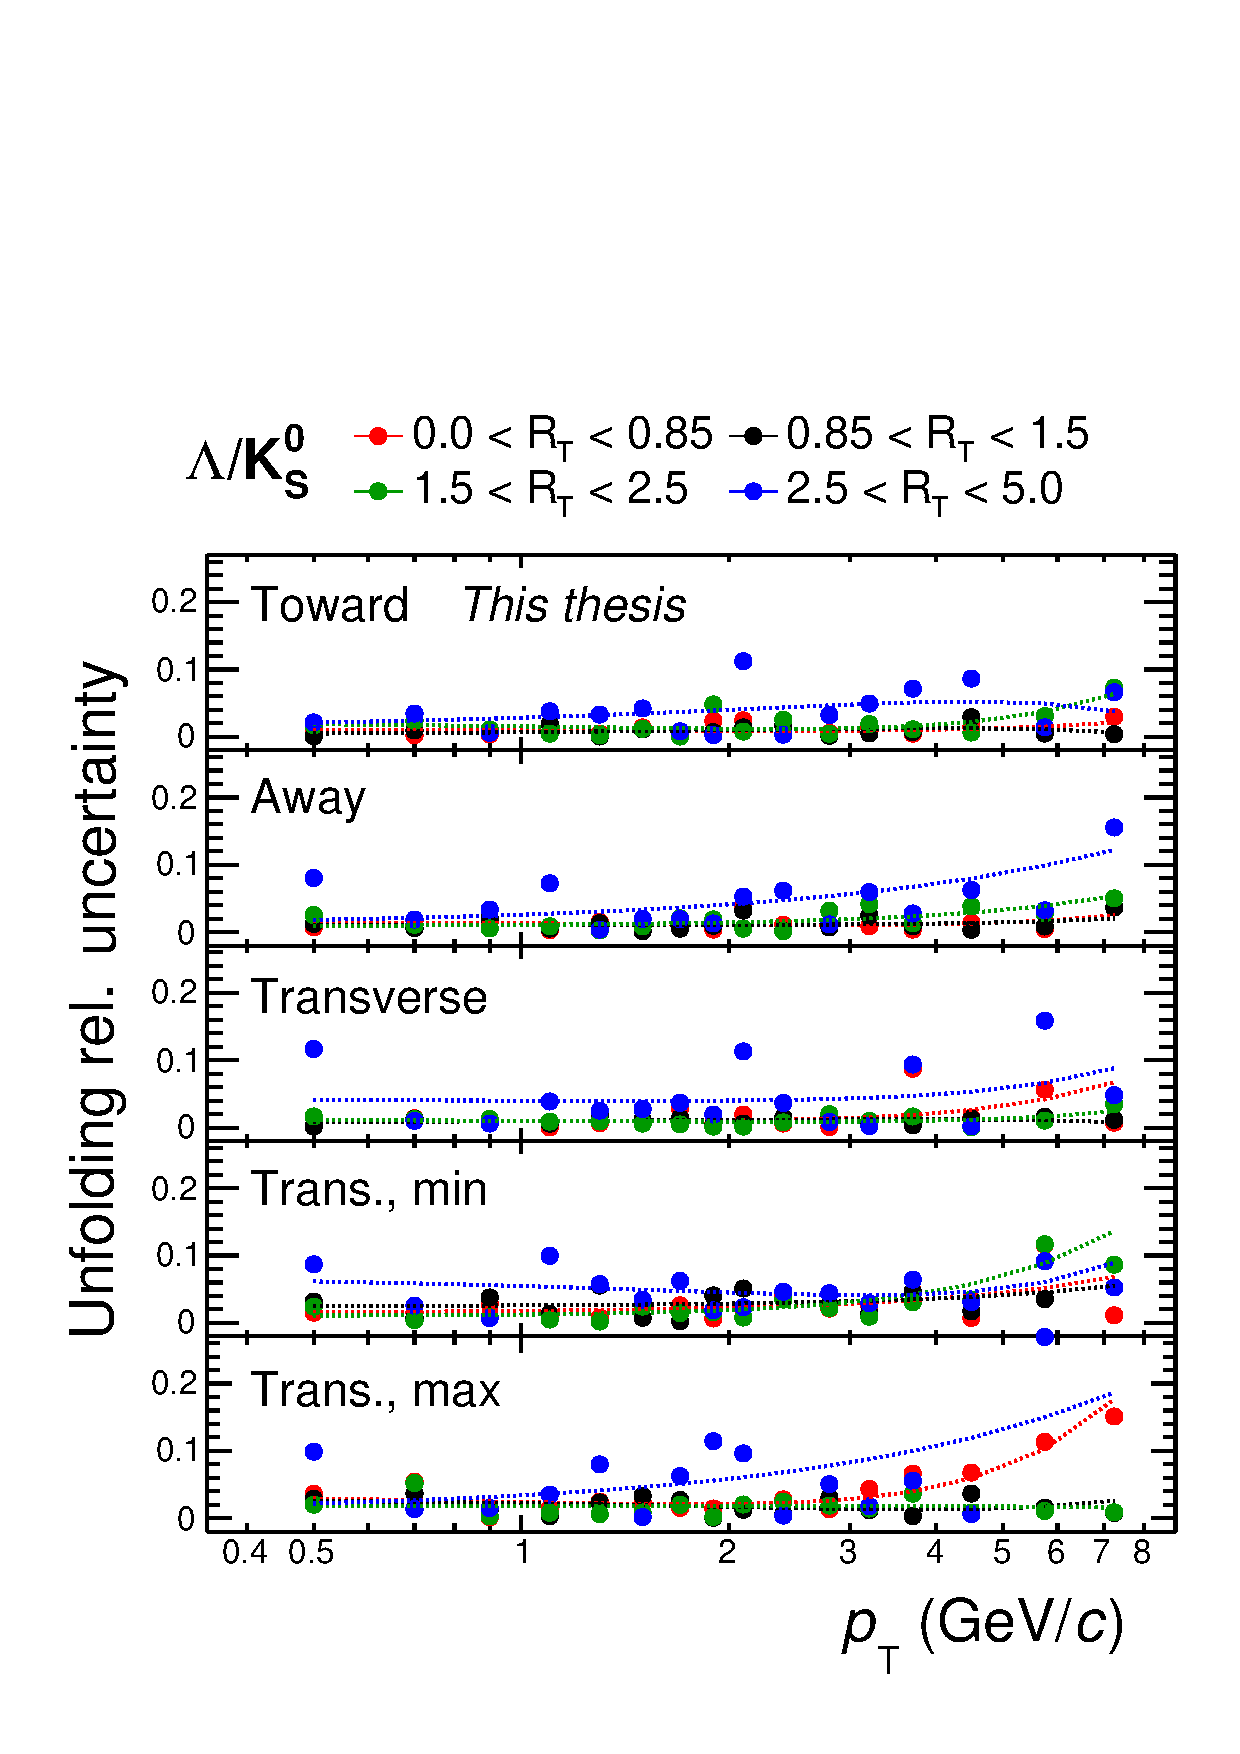
\includegraphics[width=.320\textwidth]{\imgpath/InfoRT_systUnf_LtoK0s.pdf}}
\caption{Relative systematic uncertainties on transverse momentum spectra resulting from the Bayesian unfolding treatment for the \textbf{(a)} \KOs, \textbf{(b)} \LA+\AL, \textbf{(c)} and the \ltok ratio. The smoothened results obtained from first- and second-order polynomial fits are shown as dotted lines.}
\label{fig:rt:systUnf}
\end{figure}

\subsection{Uncorrelated uncertainties}

Systematic uncertainties may be largely correlated between the different \RT intervals and thus cancel to some degree when reporting ratios of \pt spectra in given \RT bins to the \RT-integrated case. To determine the uncorrelated part, the procedure outlied in Sec.~\ref{sec:ana:systunc} is followed, in the same fashion as in the \SOPT measurement. They are reported in Appendix~\ref{app:rtsystunc} and summarised in Tab.~\ref{tab:rt:syst}.

\section{Description of regions and mean transverse momentum}

After unfolding, the average transverse momenta \meanpt of \KOs and \LA were studied in the Toward, Away, Transverse, Transverse-min, and Transverse-max regions as a function of \NT, \NTmin, and \NTmax. To guide the focus of the analysis, according to MC paradigms as well as previous UE measurements \cite{fieldUnderlyingEventHadronic2012, ortizEnergyDependenceUnderlyingevent2021}, the following expectations were considered on the origin of the particles:
\begin{enumerate}
\item \textit{Toward and Away regions}: particles from jet fragmentation and underlying event.
\item \textit{Transverse region}: particles from UE, which includes contributions from softer MPIs and harder wide-angle initial- and final-state radiation.
\item \textit{Transverse-min region}: particles from UE, where the softer MPI contribution dominates.
\item \textit{Transverse-max region}: particles from UE biased towards higher amounts of harder ISR/FSR.
\end{enumerate}

The choice of the independent observable is then expected to focus on the effects of:
\begin{enumerate}
\item \textit{Toward and Away regions}: for all \NT, \NTmin, and \NTmax, mixing the relative contributions of UE and jet fragmentation.
\item \textit{Transverse(-min,max) regions}: for \NT, the magnitude of the inclusive UE, for \NTmin, the magnitude of the softer-MPIs-enhanced MPI, and for \NTmax, the magnitude of the harder-ISR/FSR-biased UE.
\end{enumerate}

Fig.~\ref{fig:rt:meanptK0s} shows the \KOs \meanpt results for different configurations. In the Toward and Away regions, the dependence on \NT, \NTmin, and \NTmax appears comparable, exhibiting a "jet peak" at low \NT and a flow-like boost from the underlying event at high \NT values. In the Transverse, Transverse-min, and Transverse-max regions, \meanpt steeply increases with \NT, with an ordering in terms of absolute values, although the slopes are similar. These results suggest that the choice of particle region does not have a significant impact on its dynamical properties.

Additionally, the increase in \meanpt with \NTmax is much steeper in the Transverse-max region compared to the Transverse-min region's increase with \NTmin, indicating that the choice of independent variable plays the more important role. Together with the choice of particle region, it has the potential to isolate distinct behaviors between the two activity extremes.

Given these findings, this dissertation focuses on the following measurements: Toward/Away/Transverse versus \RT (\NT), Transverse-min versus \RTmin (\NTmin), and Transverse-max versus \RTmax (\NTmax).

Alternatively, the \meanpt values can be calculated by a re-weighting procedure, which determines \meanpt on the pre-unfolded spectra and then sums them together with weights obtained from the smearing matrix \cite{alicecollaborationUnderlyingEventProperties2020}. However, this method was not pursued in this dissertation. 

\begin{figure}[H]%
\subfloat[][]{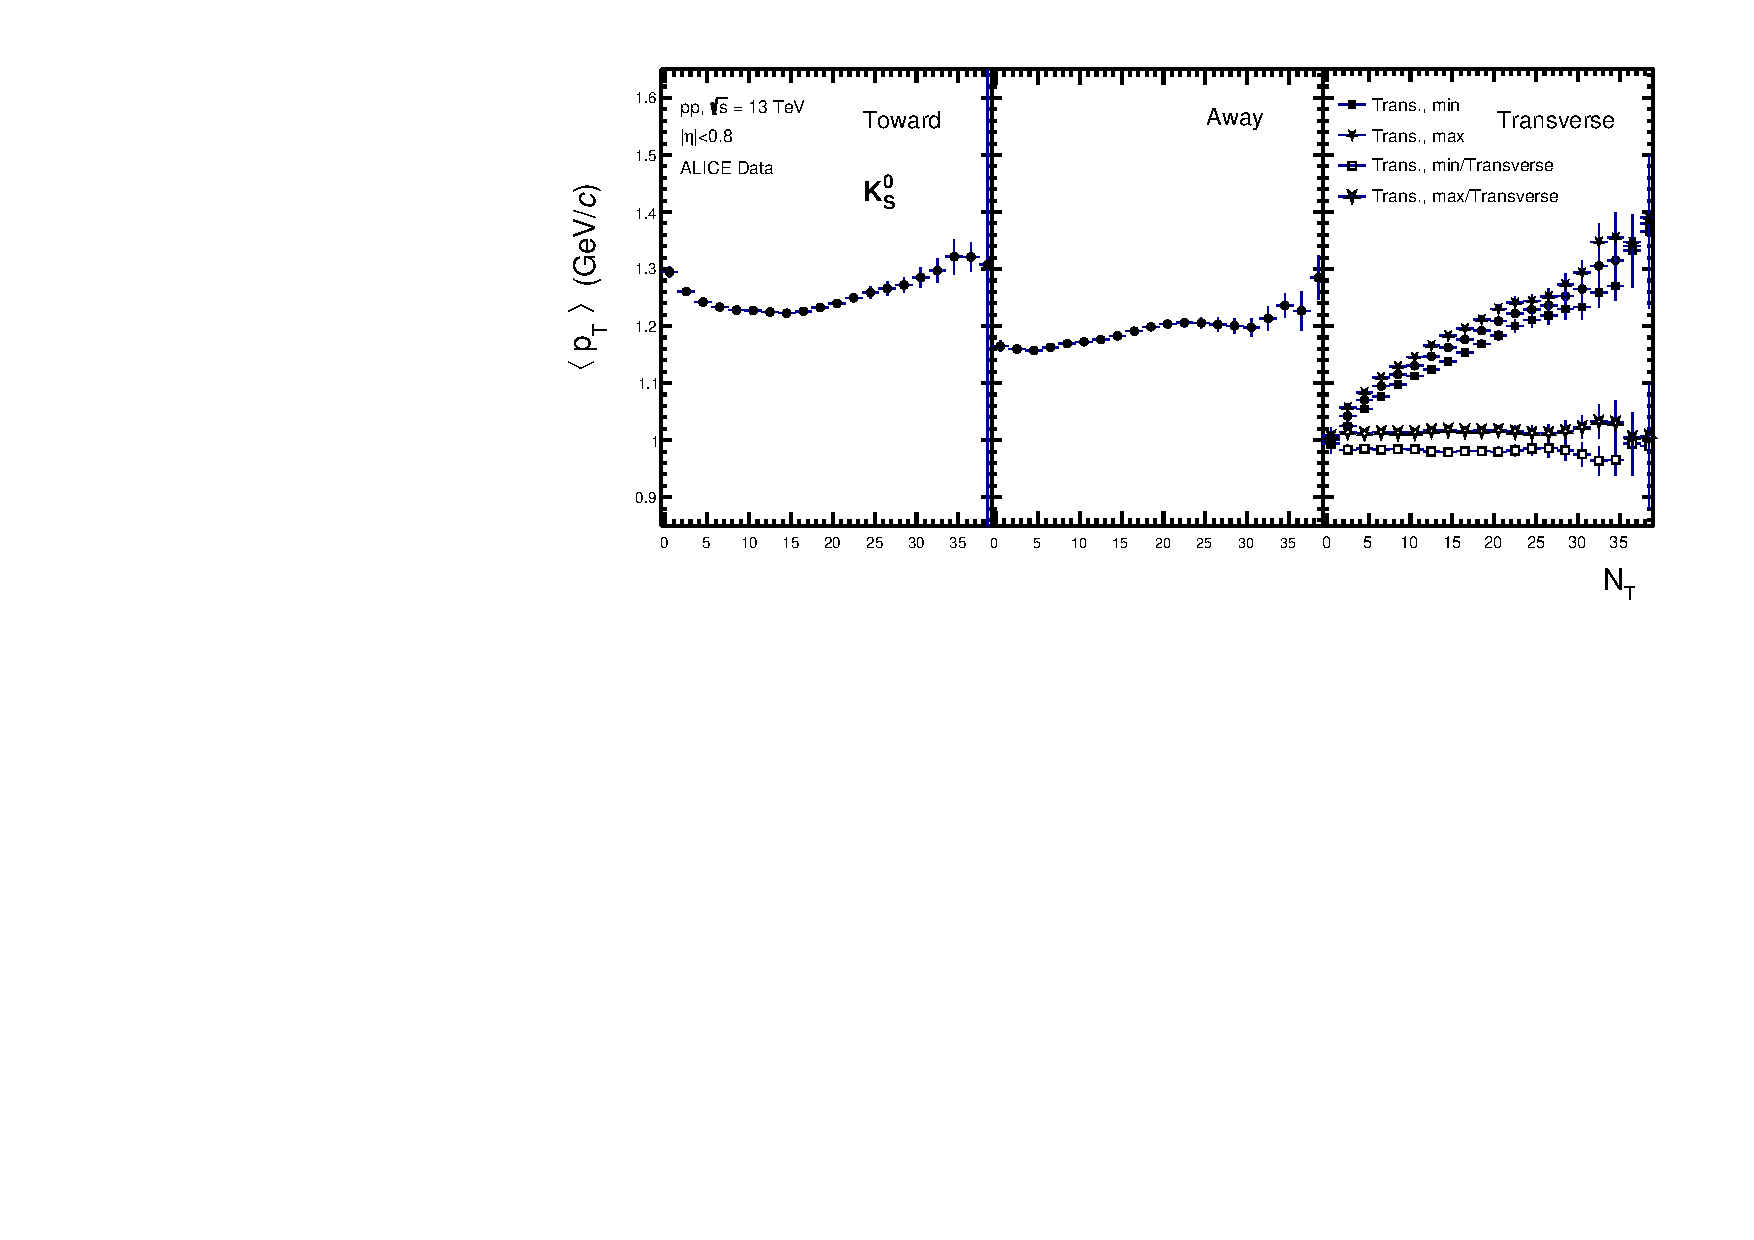
\includegraphics[width=.90\textwidth]{\imgpath/PtvNt_MeanPt_0_K0s.pdf}}\\
\subfloat[][]{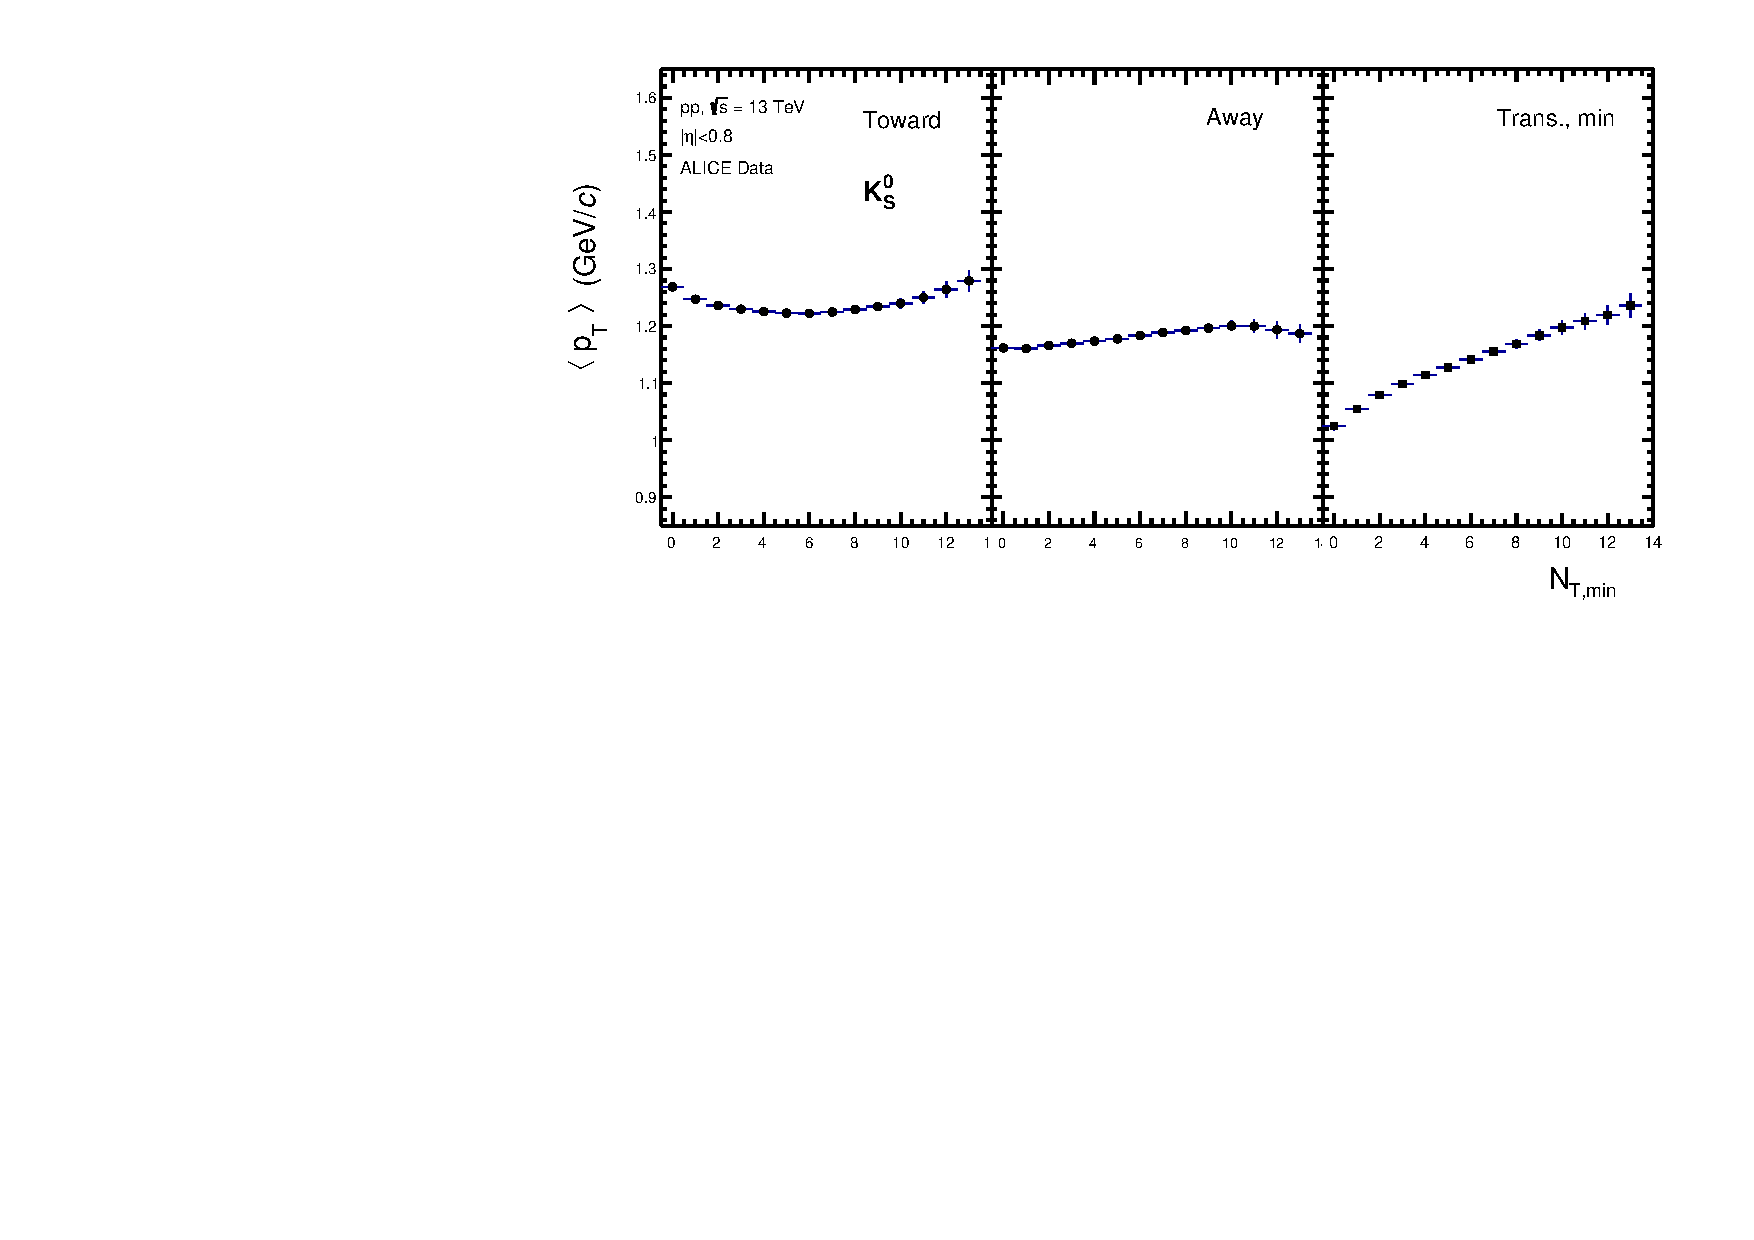
\includegraphics[width=.90\textwidth]{\imgpath/PtvNt_MeanPt_1_K0s.pdf}}\\
\subfloat[][]{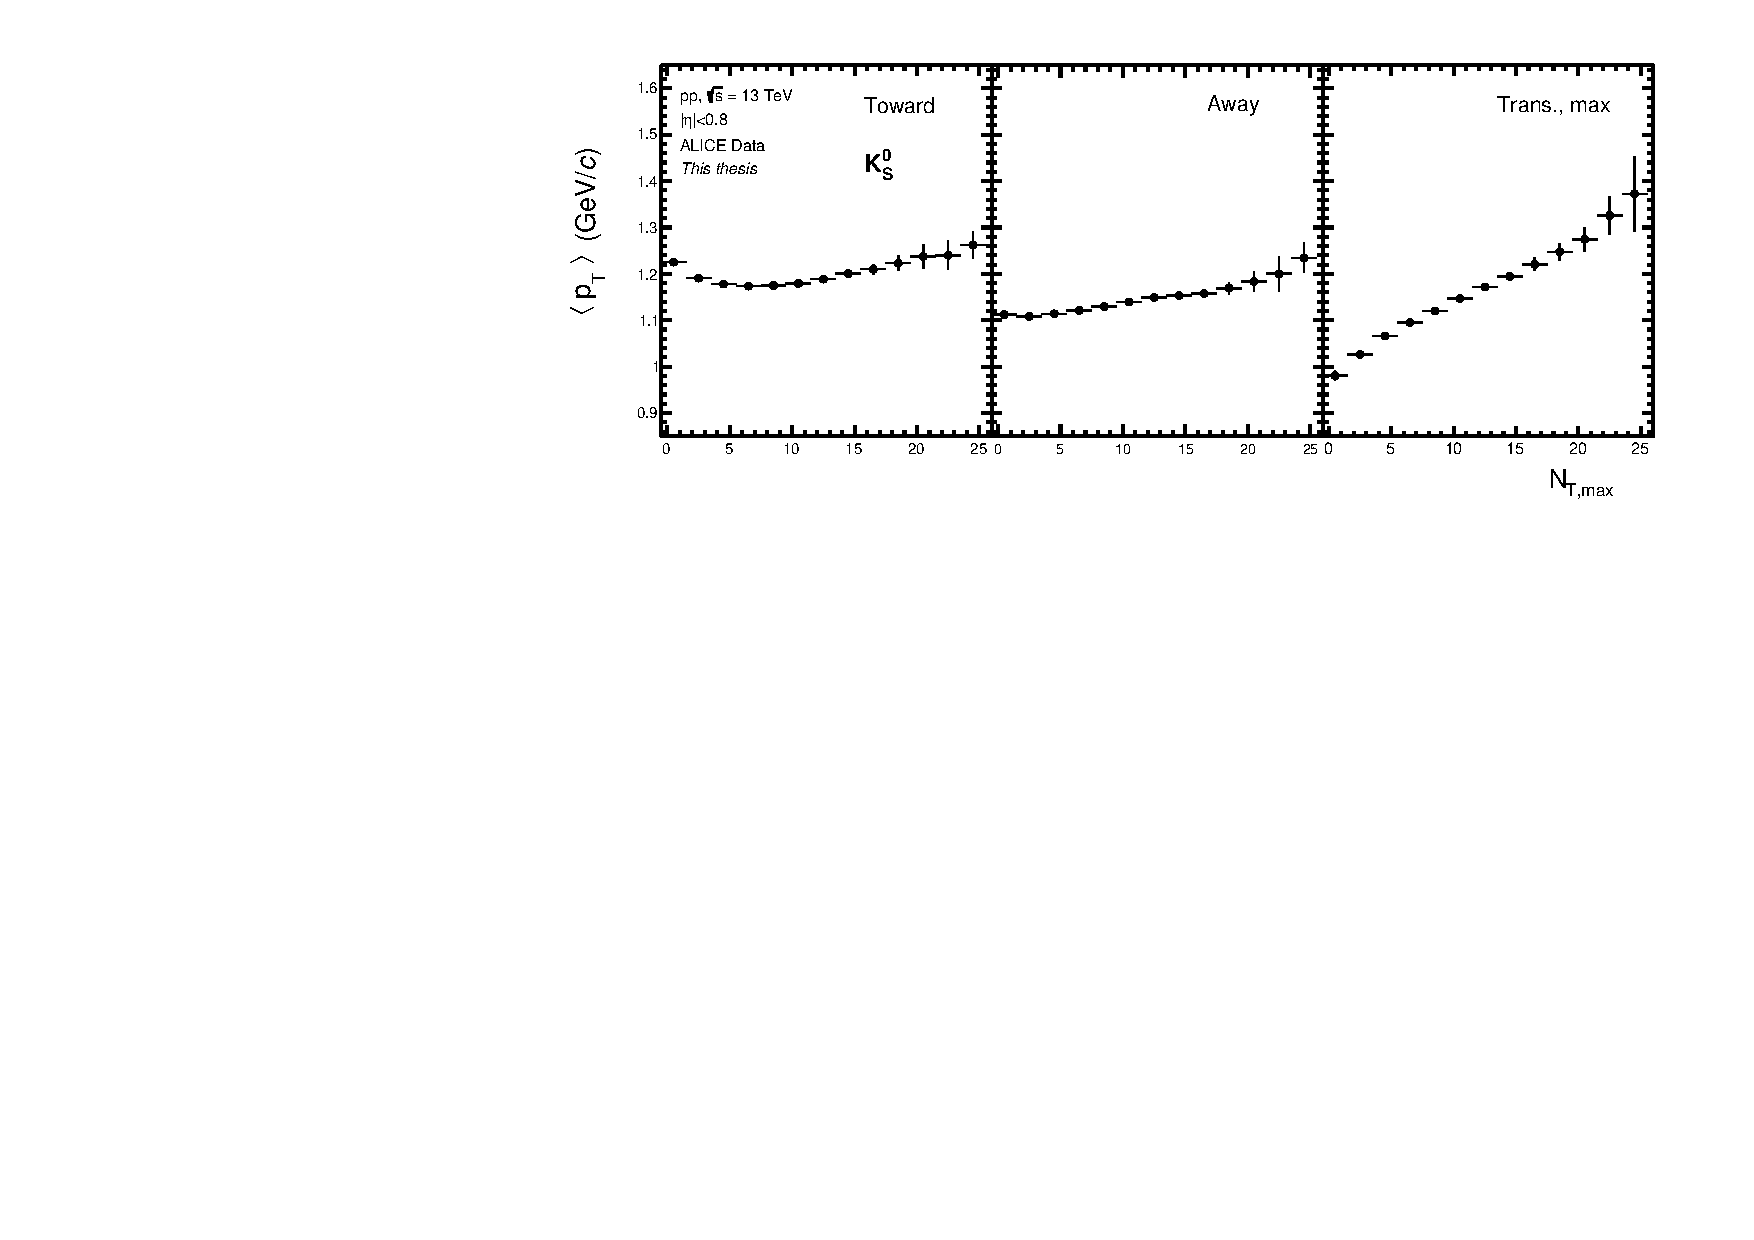
\includegraphics[width=.90\textwidth]{\imgpath/PtvNt_MeanPt_2_K0s.pdf}}\\
\caption{Mean transverse momentum for \KOs as a function of \textbf{(a)} \NT, \textbf{(b)} \NTmin, \textbf{(c)} \NTmax in the different azimuthal regions. The x-axis ranges were chosen such that they represent comparable quantiles of the distributions of their variables, to facilitate a more direct comparison. Only statistical uncertainties are presented and systematic biases on \meanpt from the unfolding treatment were not considered.}
\label{fig:rt:meanptK0s}
\end{figure}

\section{Transverse momentum spectra}

The measured \pt spectra for \KOs and \LA, after applying all corrections and accounting for systematic uncertainties, are presented in Fig.\ref{fig:rt:ptK0s} and Fig.\ref{fig:rt:ptLA}, respectively. In addition, these spectra are compared with model predictions in Fig.\ref{fig:rt:ptK0sMC} and Fig.\ref{fig:rt:ptLAMC}.

In the Toward and Away regions, there is a dependence at intermediate \pt, followed by a convergence "to a jet" at high \pt. This suggests that high-momentum particles solely originating from jets are independent of the UE, as expected. The Transverse region exhibit an increase and hardening with increasing \RT, indicating that events with higher UE activity are more likely to contain higher-\pt particles. This trend is similar to studies of charged particles at mid-rapidity as a function of \Nch measured at mid-rapidity, where the auto-correlation bias is an important factor in interpretation.

The behavior of the Transverse-max region is similar to that of the Transverse region, indicating the selection of harder wide-angle ISR/FSR. However, the Transverse-min region seems to plateau, suggesting that at higher \pt, \RTmin does not impact the particle \pt spectral shapes.

When compared with MC predictions including Pythia Monash, Pythia Ropes, and EPOS LHC, all models reproduce the data qualitatively very well, although quantitative differences can be noticed.

Finally, it is also interesting to remember Pythia and Herwig predictions for inclusive charged particles shown in Fig.~\ref{fig:rt:nchpt}, which showed a steady hardening in high-UE events in the Transverse and Transverse-max regions, whereas a Cronin-like peak was observed for the Transverse-min case. The data reported here offer some support to these expectations but do not explicitely confirm them, suggesting that even higher \RTmin values are needed.

\begin{figure}[H]%
\subfloat[][]{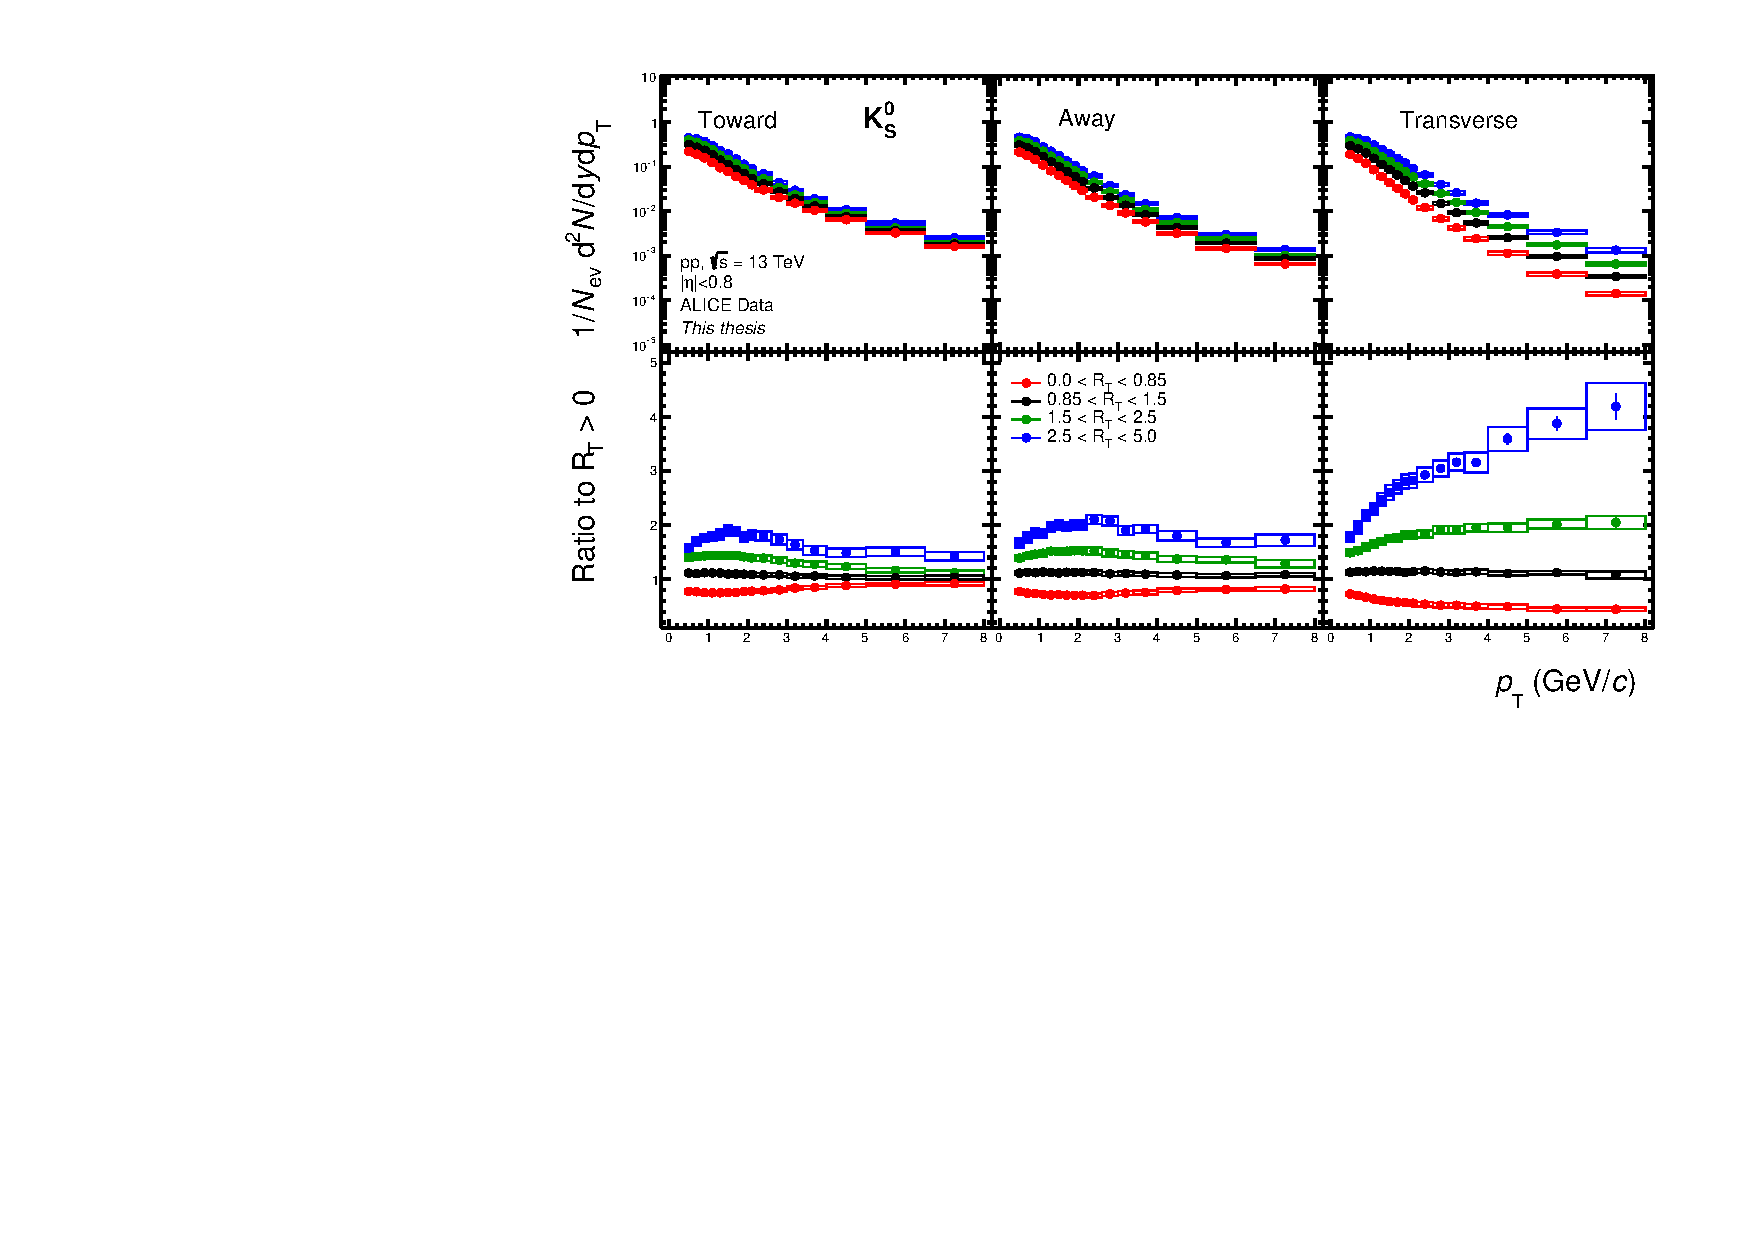
\includegraphics[width=.990\textwidth]{\imgpath/PtvRt_Pt_K0s.pdf}}\\
\subfloat[][]{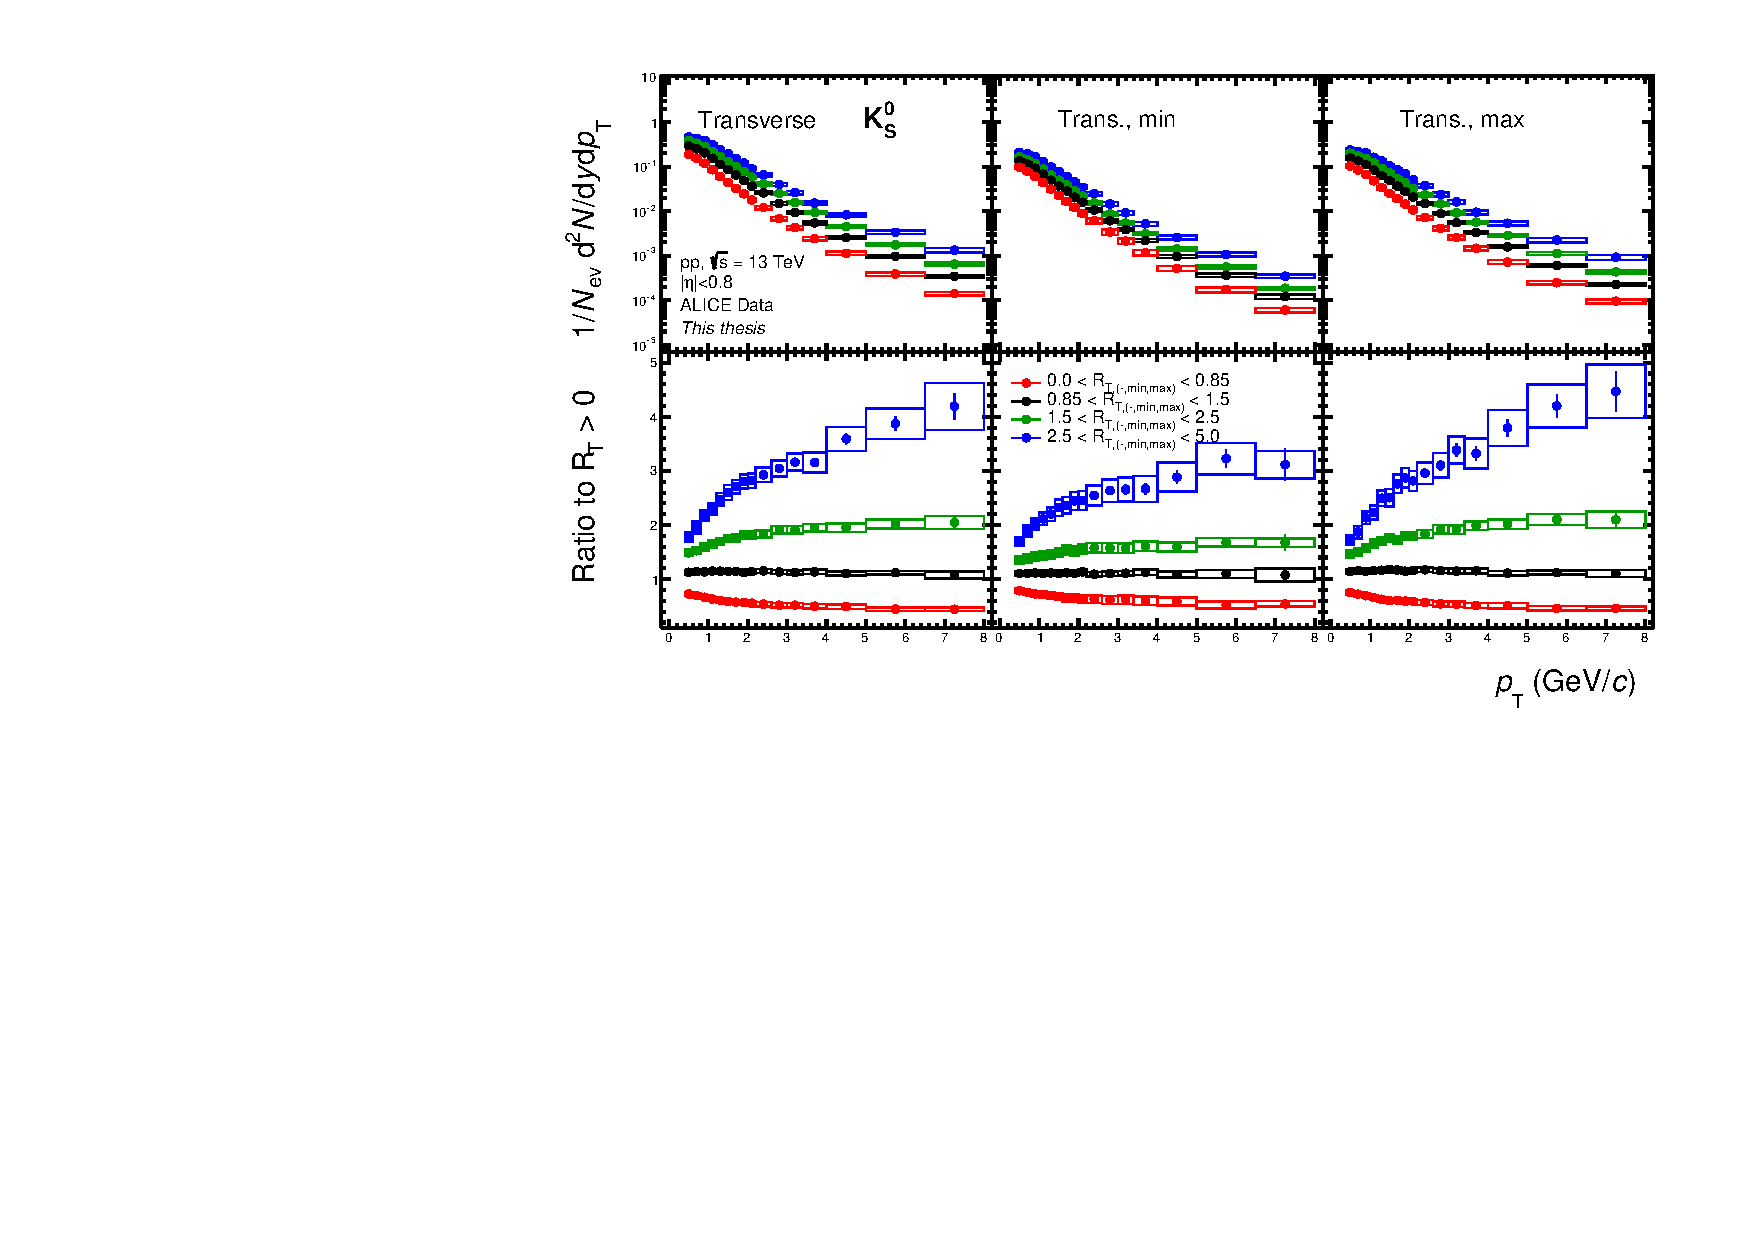
\includegraphics[width=.990\textwidth]{\imgpath/PtvRt_Pt2_K0s.pdf}}\\
\caption{Transverse momentum spectra of \KOs for different \RT/\RTmin/\RTmax intervals in pp collisions at \sppt{13} in \textbf{(a)} Toward, Away, and Transverse, \textbf{(b)} Transverse, Transverse-min, and Transverse-max regions. The bottom panels display ratios to the \RT/\RTmin/\RTmax-integrated cases. The error bars represent statistical uncertainties and the rectangles show the systematic uncertainties.}
\label{fig:rt:ptK0s}
\end{figure}


\begin{figure}[H]%
\subfloat[][]{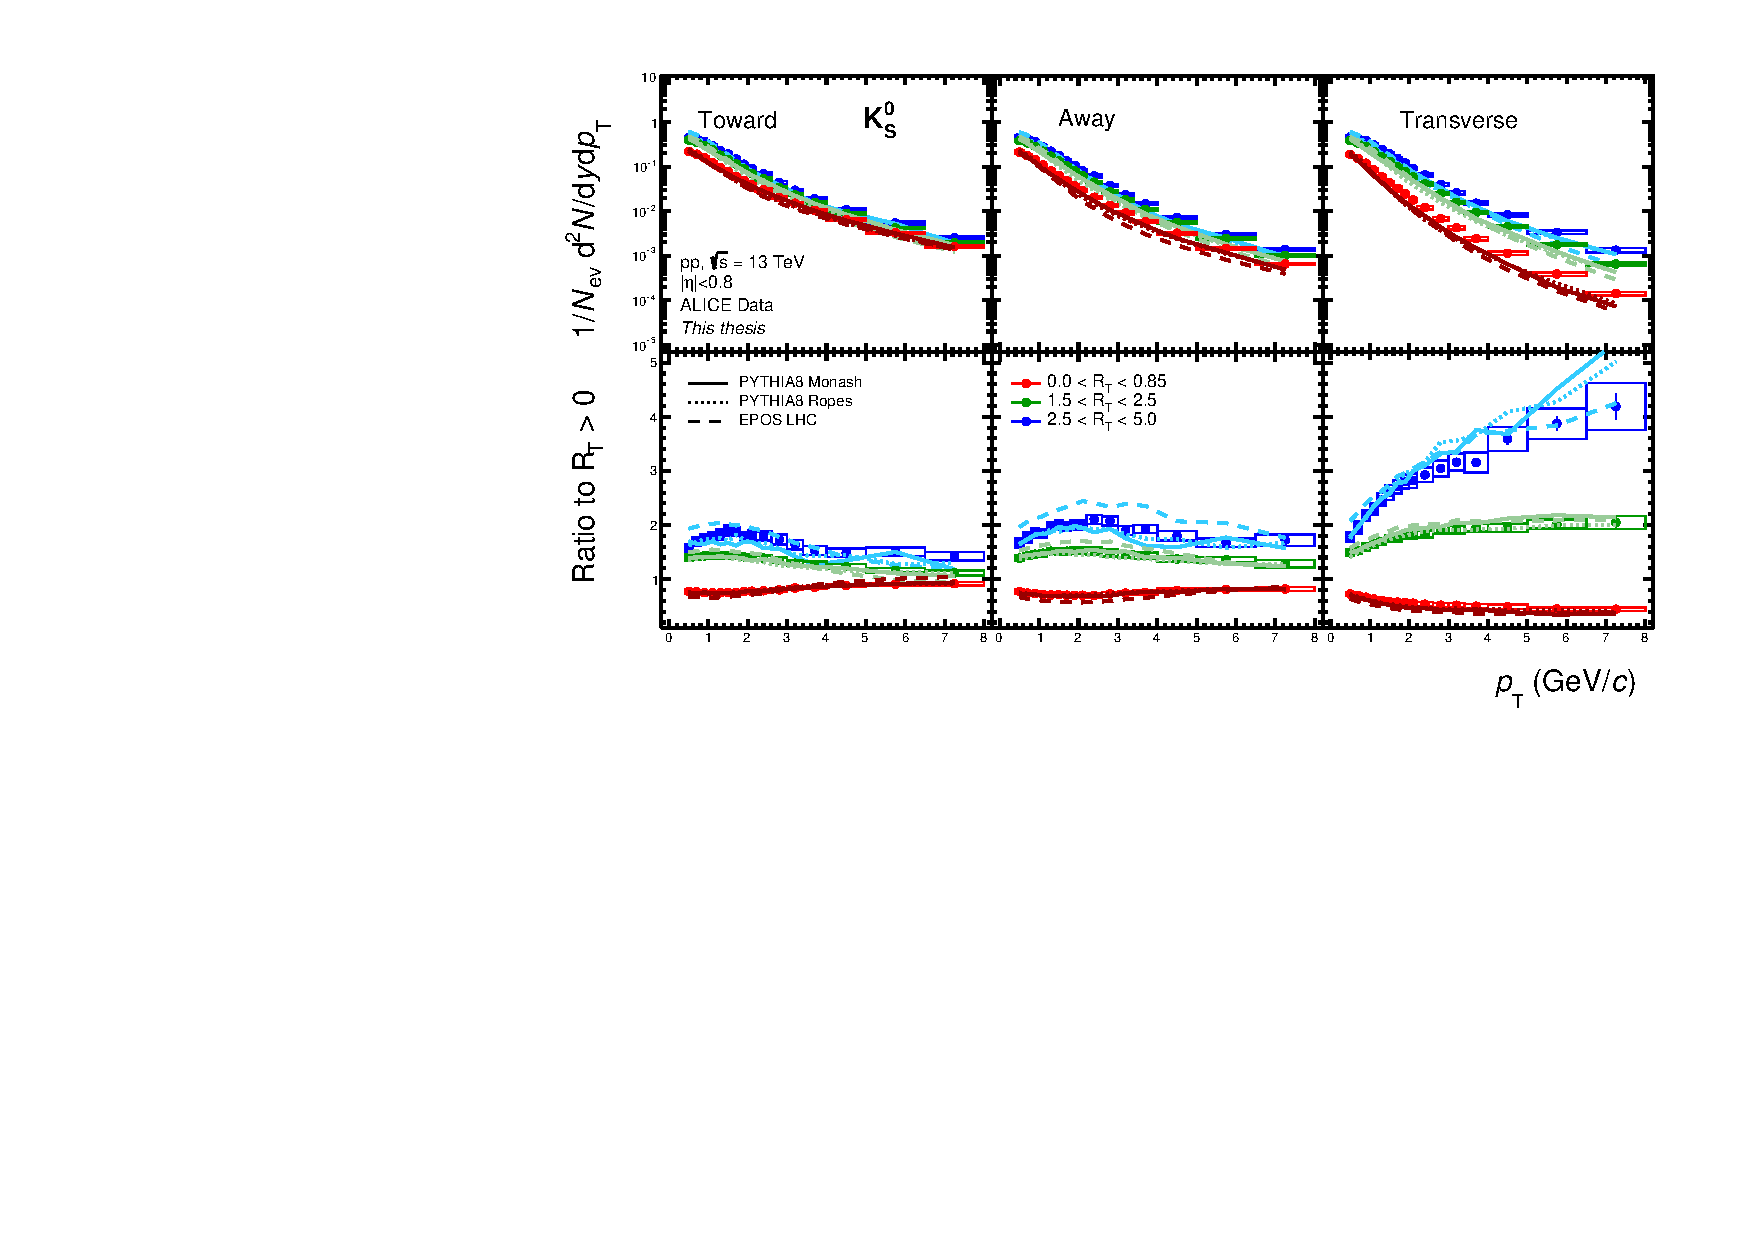
\includegraphics[width=.990\textwidth]{\imgpath/PtvRt_PtMC_K0s.pdf}}\\
\subfloat[][]{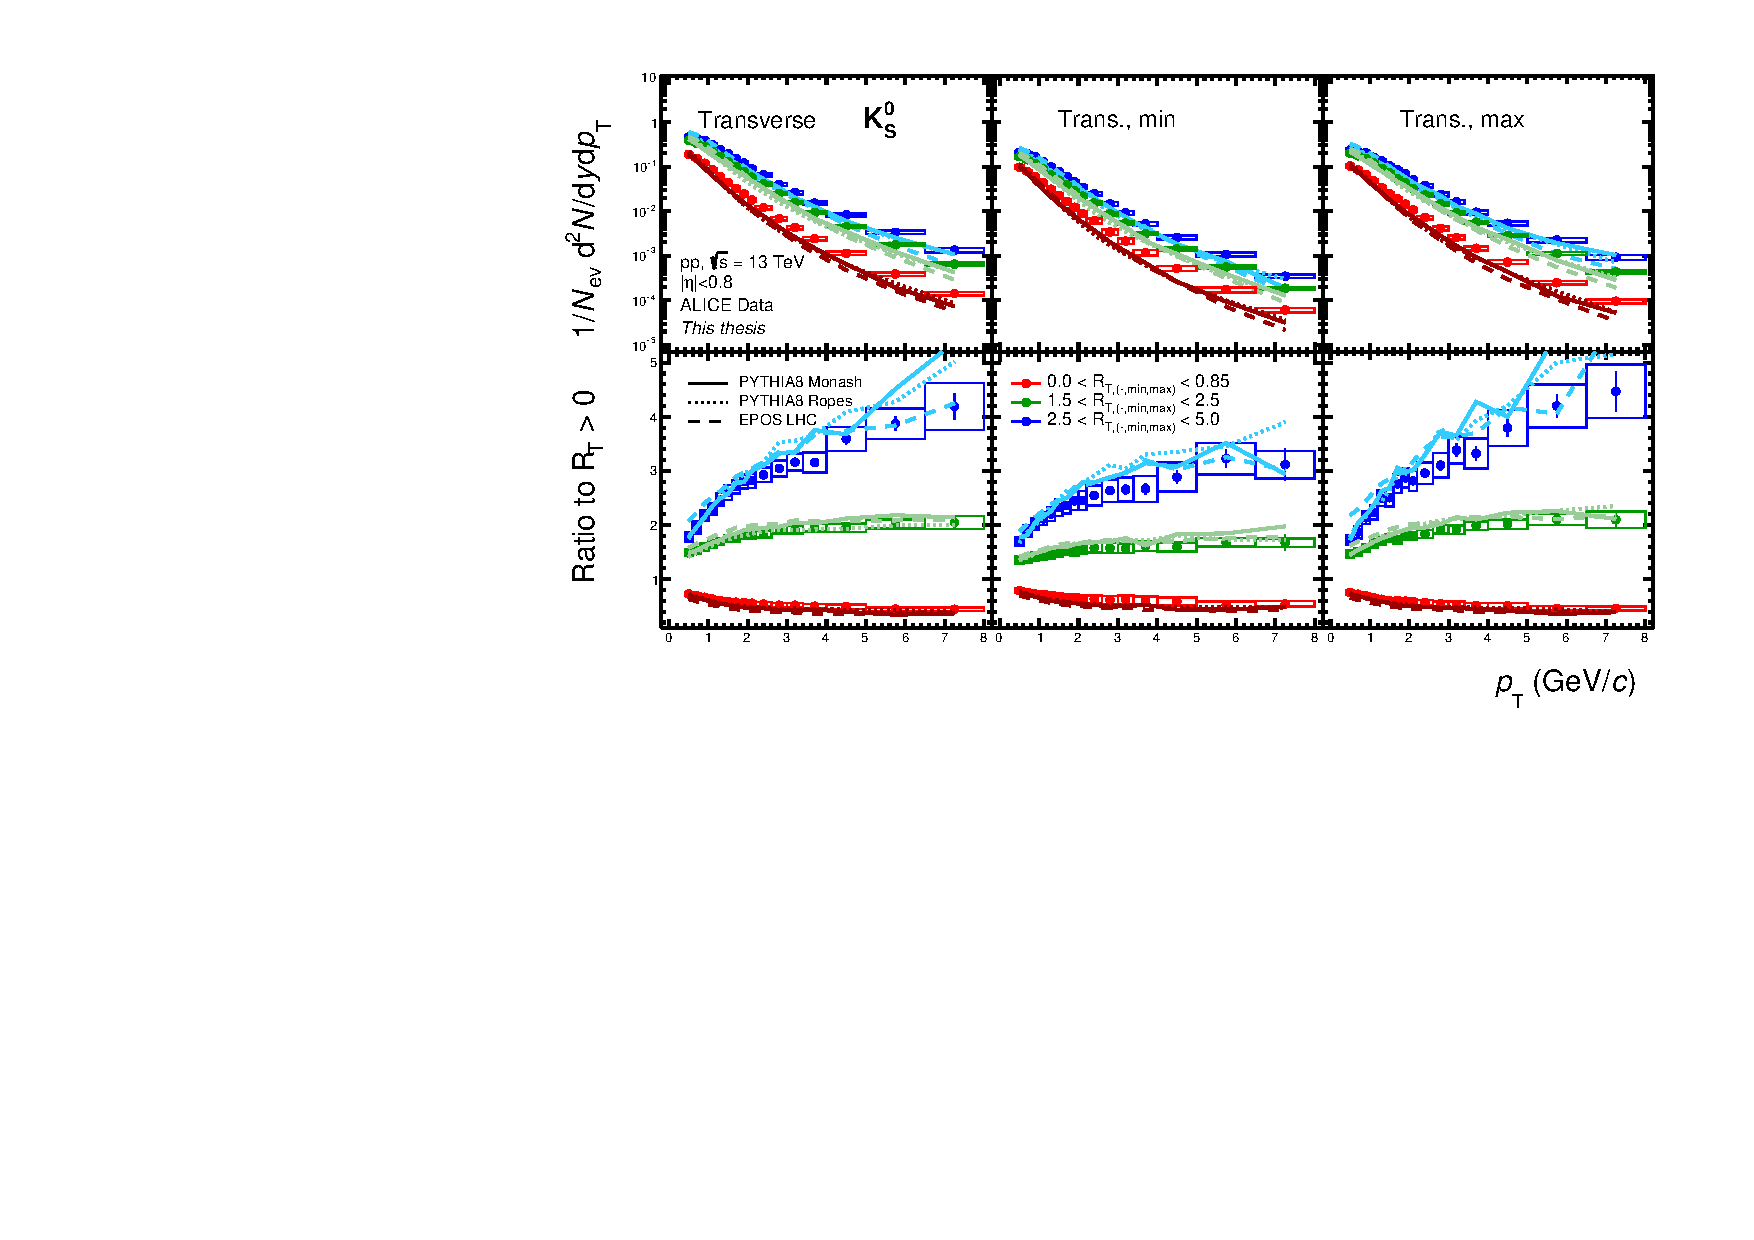
\includegraphics[width=.990\textwidth]{\imgpath/PtvRt_PtMC2_K0s.pdf}}\\
\caption{Transverse momentum spectra of \KOs for different \RT/\RTmin/\RTmax intervals in pp collisions at \sppt{13} compared with MC predictions in \textbf{(a)} Toward, Away, and Transverse, \textbf{(b)} Transverse, Transverse-min, and Transverse-max regions. The bottom panels display ratios to the \RT/\RTmin/\RTmax-integrated cases. The error bars represent statistical uncertainties and the rectangles show the systematic uncertainties.}
\label{fig:rt:ptK0sMC}
\end{figure}

\begin{figure}[H]%
\subfloat[][]{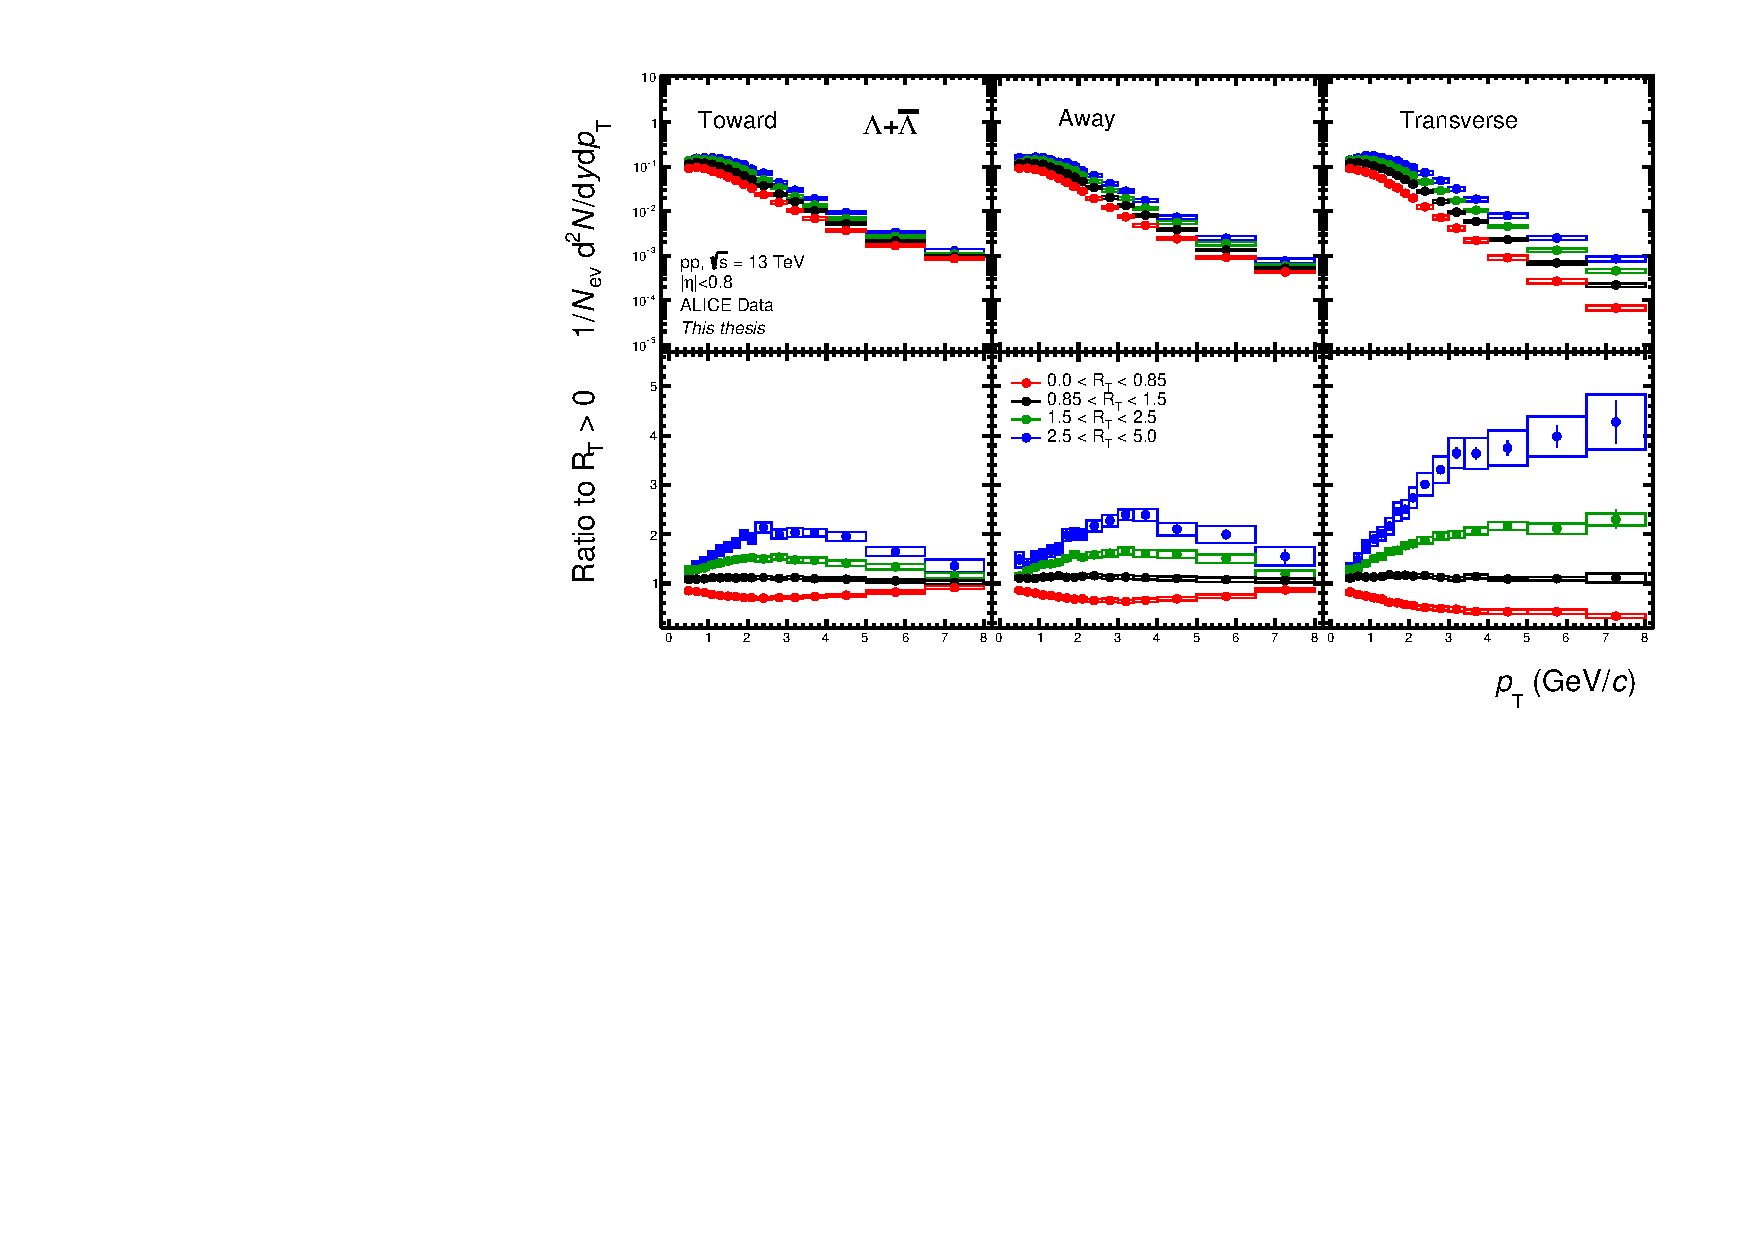
\includegraphics[width=.990\textwidth]{\imgpath/PtvRt_Pt_L.pdf}}\\
\subfloat[][]{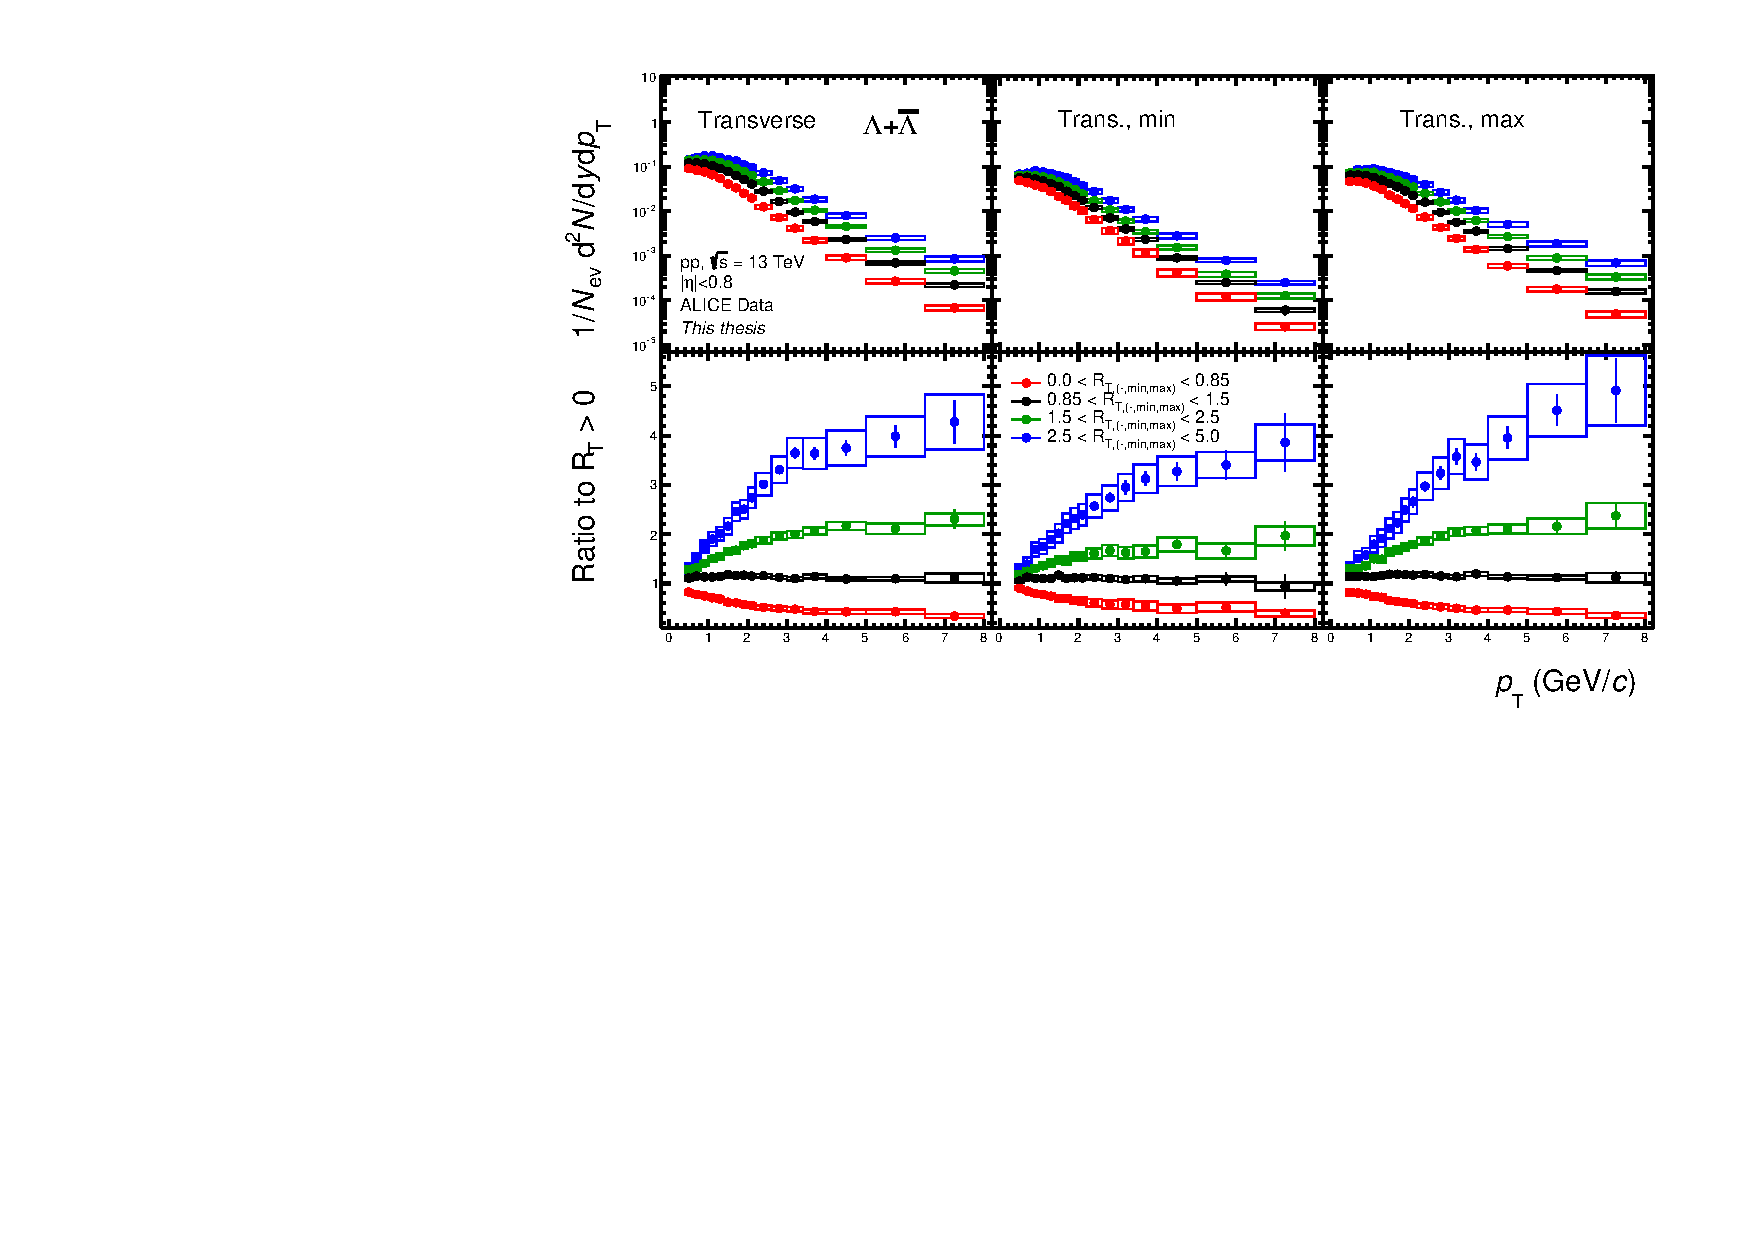
\includegraphics[width=.990\textwidth]{\imgpath/PtvRt_Pt2_L.pdf}}\\
\caption{Transverse momentum spectra of \LA+\AL for different \RT/\RTmin/\RTmax intervals in pp collisions at \sppt{13} in \textbf{(a)} Toward, Away, and Transverse, \textbf{(b)} Transverse, Transverse-min, and Transverse-max regions. The bottom panels display ratios to the \RT/\RTmin/\RTmax-integrated cases. The error bars represent statistical uncertainties and the rectangles show the systematic uncertainties.}
\label{fig:rt:ptLA}
\end{figure}


\begin{figure}[H]%
\subfloat[][]{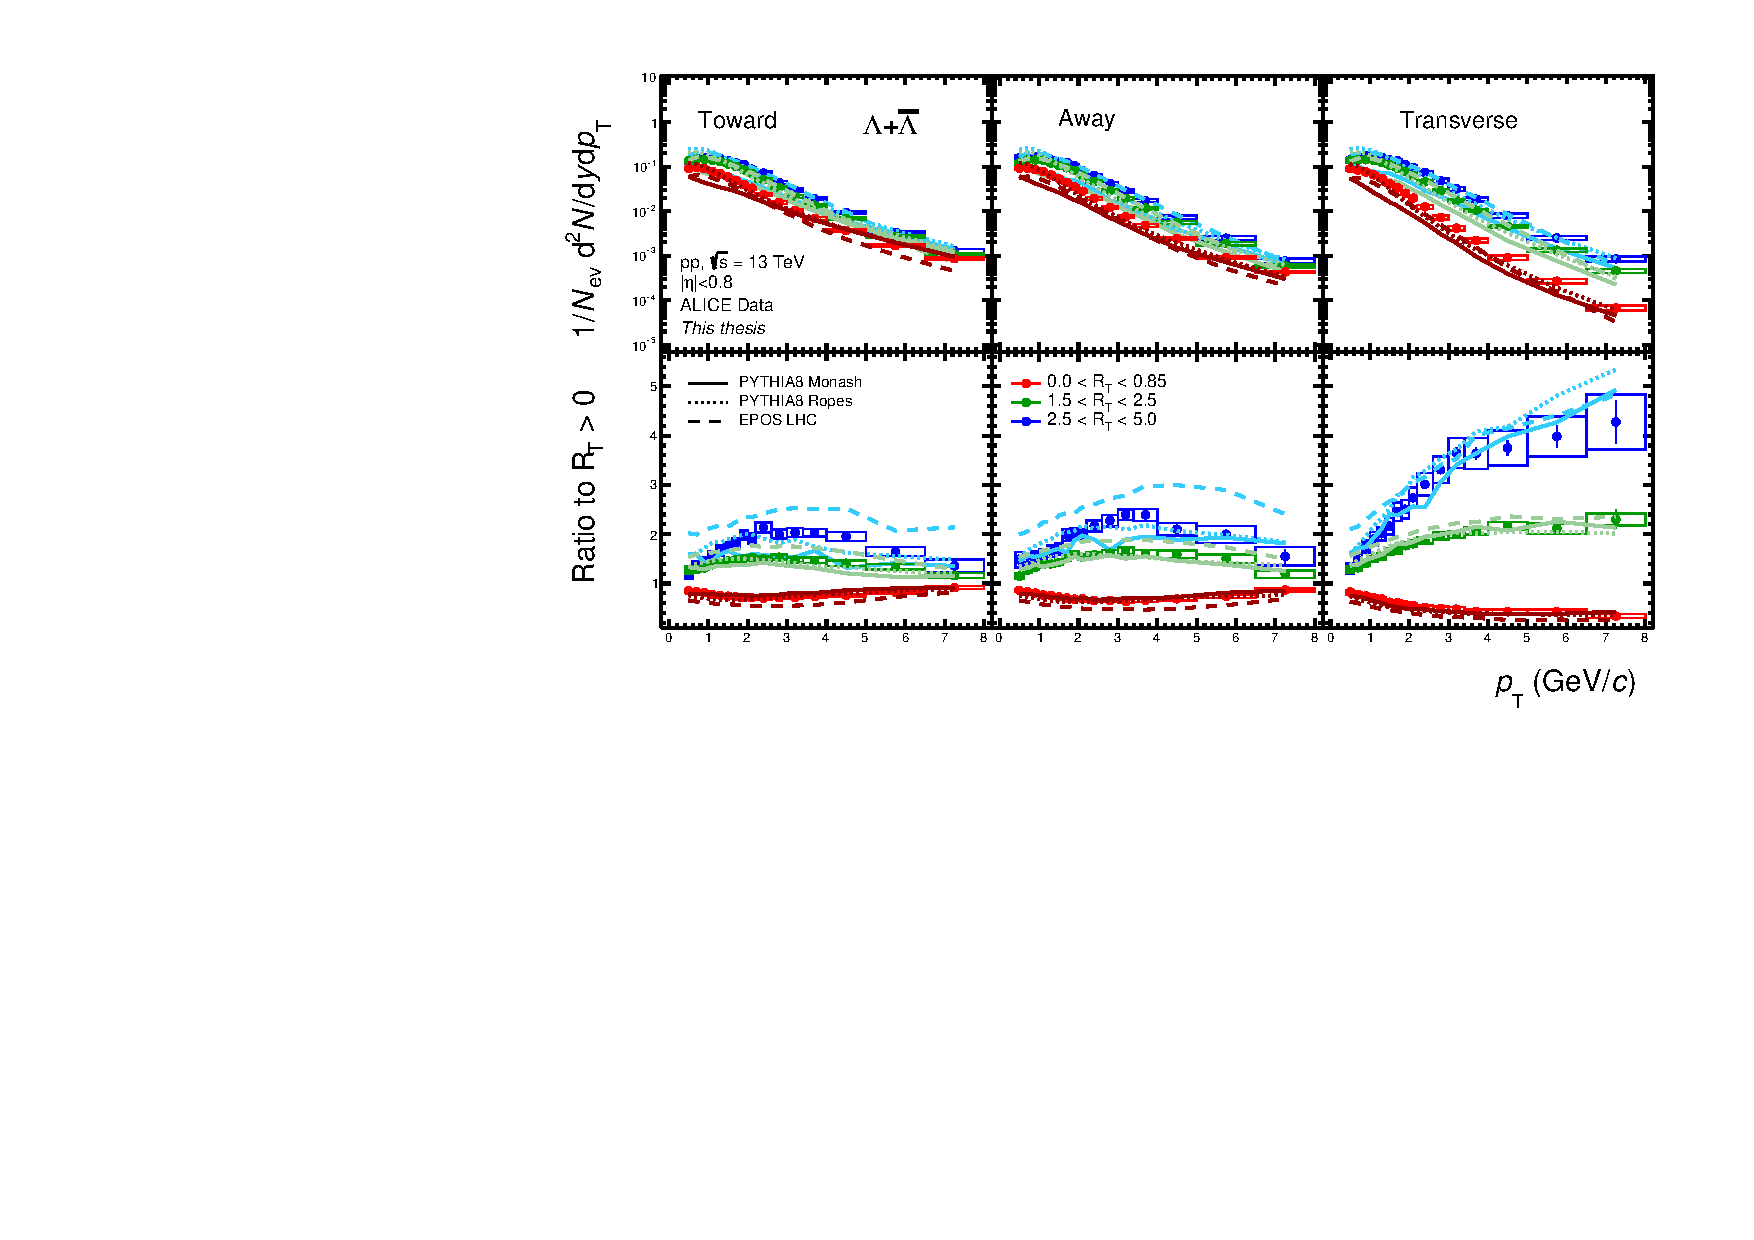
\includegraphics[width=.990\textwidth]{\imgpath/PtvRt_PtMC_L.pdf}}\\
\subfloat[][]{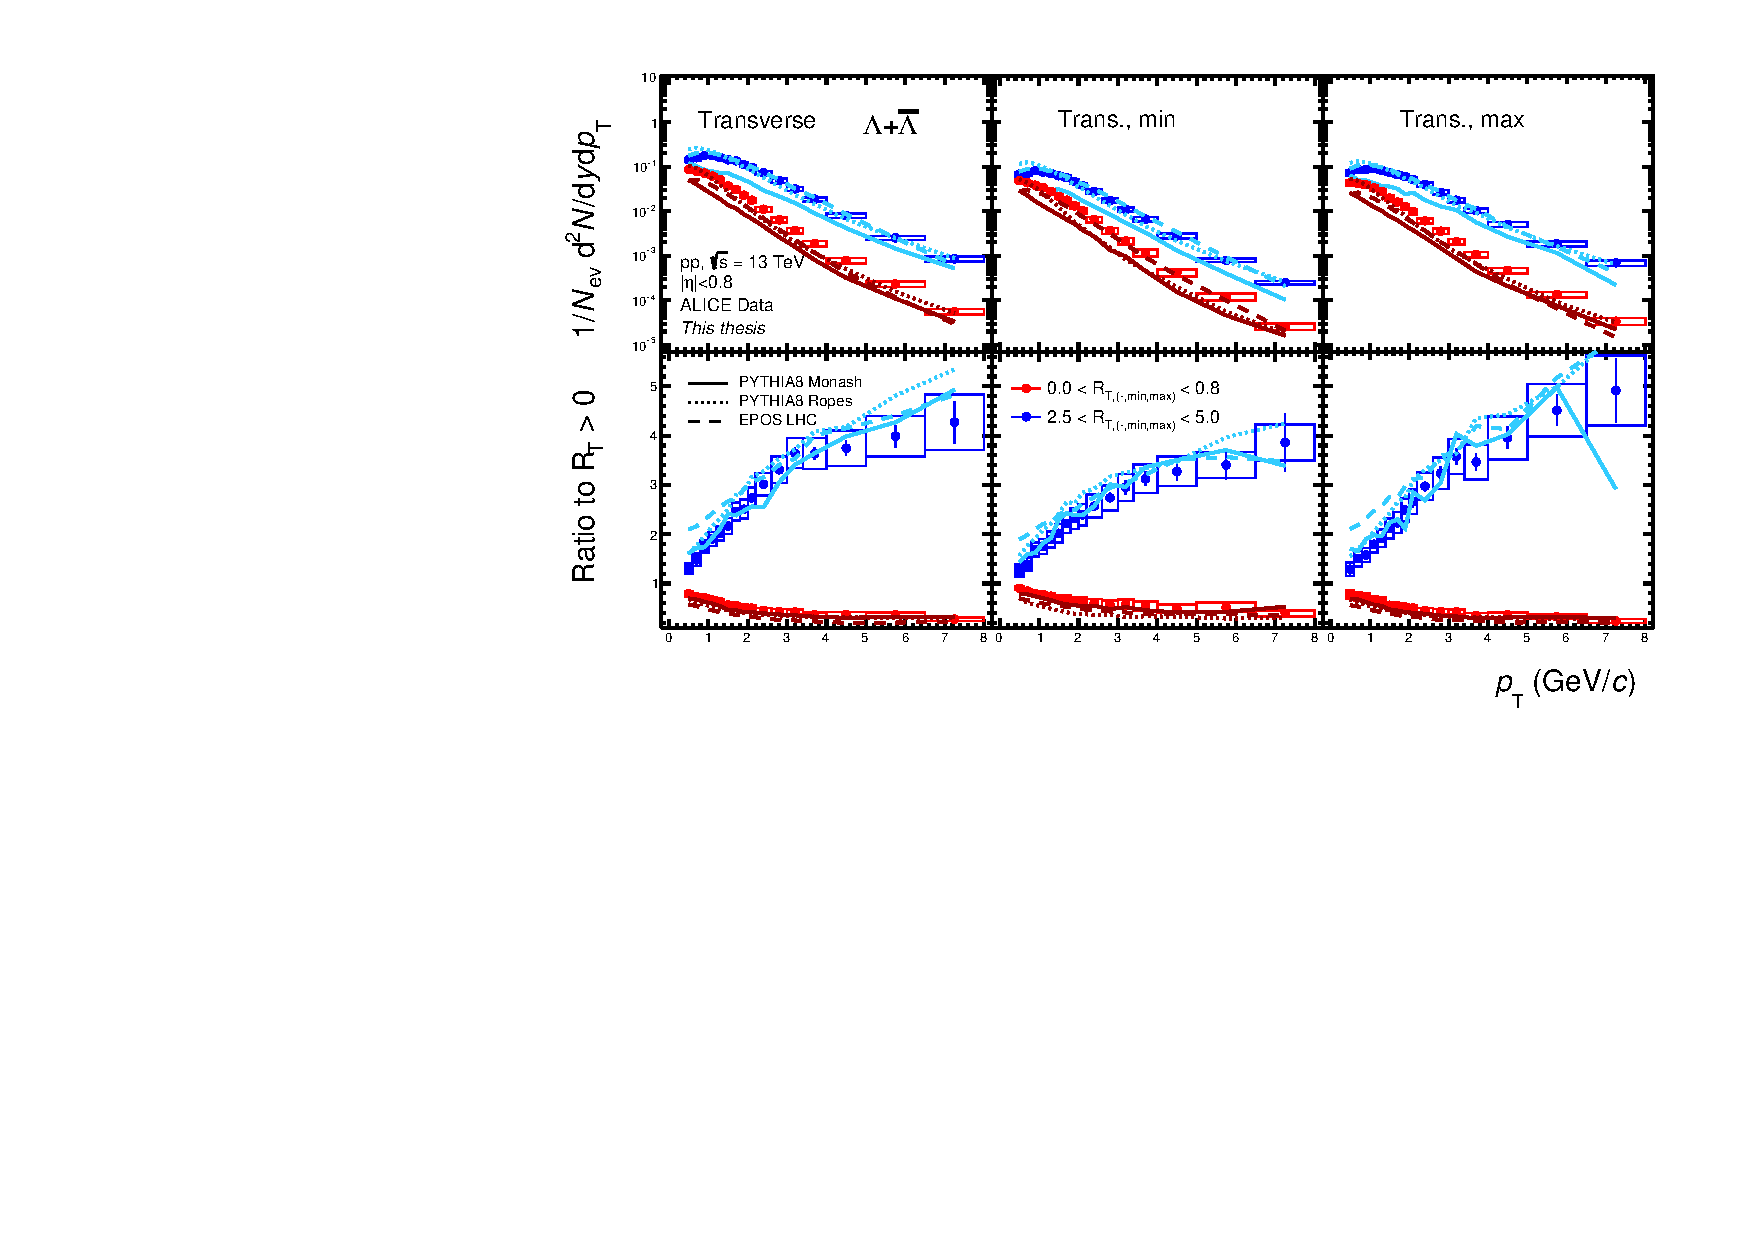
\includegraphics[width=.990\textwidth]{\imgpath/PtvRt_PtMC2_L.pdf}}\\
\caption{Transverse momentum spectra of \LA+\AL for different \RT/\RTmin/\RTmax intervals in pp collisions at \sppt{13} compared with MC predictions in \textbf{(a)} Toward, Away, and Transverse, \textbf{(b)} Transverse, Transverse-min, and Transverse-max regions. The bottom panels display ratios to the \RT/\RTmin/\RTmax-integrated cases. The error bars represent statistical uncertainties and the rectangles show the systematic uncertainties.}
\label{fig:rt:ptLAMC}
\end{figure}

\section{Baryon-to-meson ratio}

To investigate the observable most directly linked to radial flow studies, the baryon-to-meson ratios, the \ltok results are presented in Fig.\ref{fig:rt:LtoK}, and model predictions are compared in Fig.\ref{fig:rt:LtoKMC}.

Noteworthily, the biggest dependence on UE activity can be observed in the Toward and Away regions. Although this may not be immediately intuitive, as one may naively expect these regions to be dominated by jets and thus insensitive to softer phenomena like radial flow, there is a somewhat straightforward interpretation. In this region, \RT controls the amount of interplay between jet-related and UE-related production, which may differ for the \KOs and \LA. Indeed, ALICE measurements of \ltok ratios inside reconstructed jet cones and outside of them reveal a drastic difference, shown in Fig.~\ref{fig:rt:ltokjets}, further suggesting that the difference in production regime plays a significant role here, rather than any collective-flow-like behavior due to increased \nmpi.

\begin{figure}[H]%
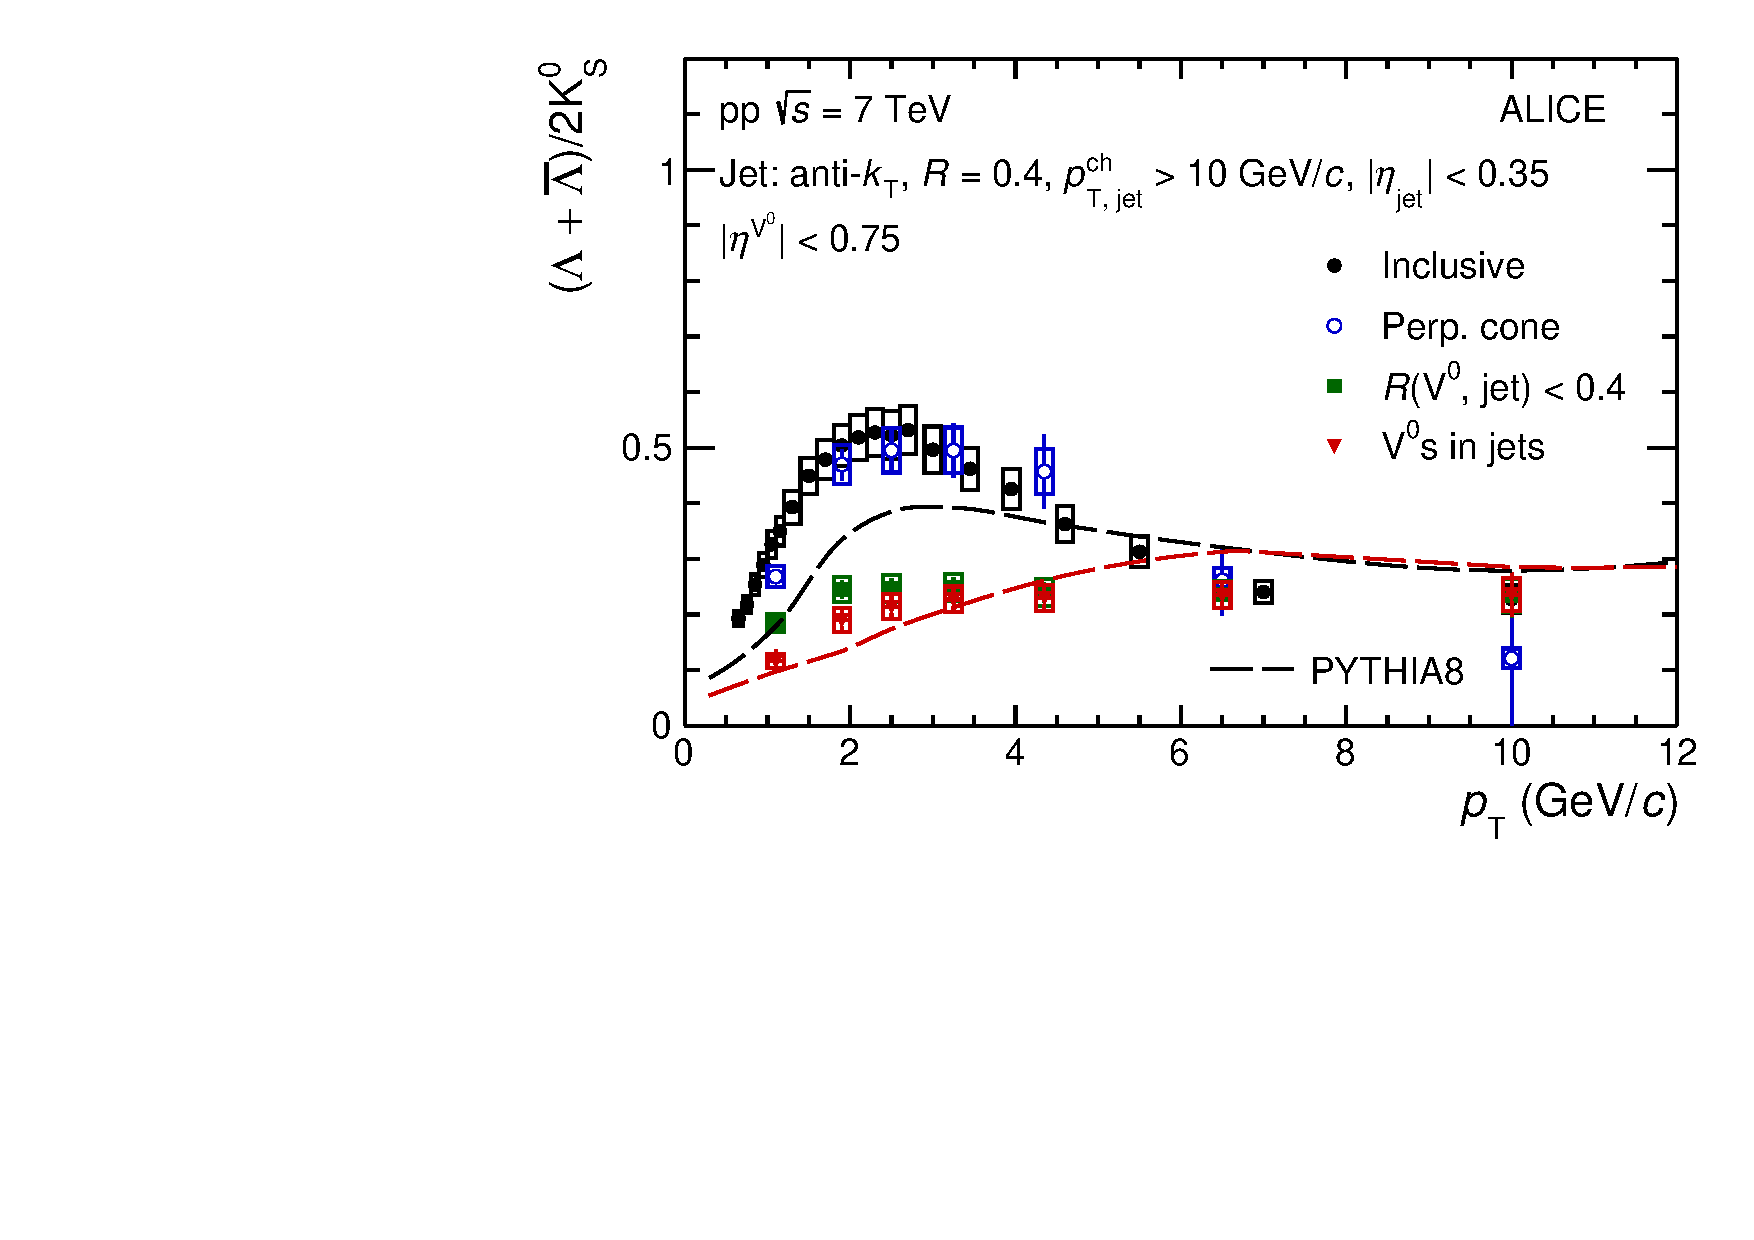
\includegraphics[width=.490\textwidth]{\imgpath/ltok_jets.pdf}\\
\caption{The \ltok ratio measured with ALICE in pp collisions at \sppt{7} in events with high-\pt jets, based on their origin: inclusive (black), inside the jet cone (green), perpendicular to the jet (blue), and in jets with the UE subtracted (red). \cite{acharyaProductionKS0Jets2022}}
\label{fig:rt:ltokjets}
\end{figure}

In contrast to the \SOPT findings, the Transverse region exhibits typical radial flow patterns: enhancement of the ratio at intermediate \pt, corresponding depletion at low \pt, and an overall shift of the peak by about $\gevc{1}$. The Transverse-min and Transverse-max regions appear to behave very similarly, with small hints of the Transverse-min exhibiting a slightly bigger effect than the Transverse-max, although the results suffer from significant statistical uncertainties. Therefore, more precise measurements are needed to confirm this observation.

Based on the selected models, the Pythia Ropes predictions are the most consistent with the data, whereas EPOS LHC exhibits a much larger dependence on \RT, and Pythia Monash significantly underestimates the ratios. The latter two models also demonstrate smaller variations of \ltok across different regions than the experimental data. Nevertheless, all the model predictions are generally consistent with describing the ratios to the \RT-integrated case. Overall, these results suggest that mechanisms that account for interactions between MPI, such as the Pythia Ropes model's implementation of increasing tension strength of many overlapping strings, are a step in the right direction.

\begin{figure}[H]%
\subfloat[][]{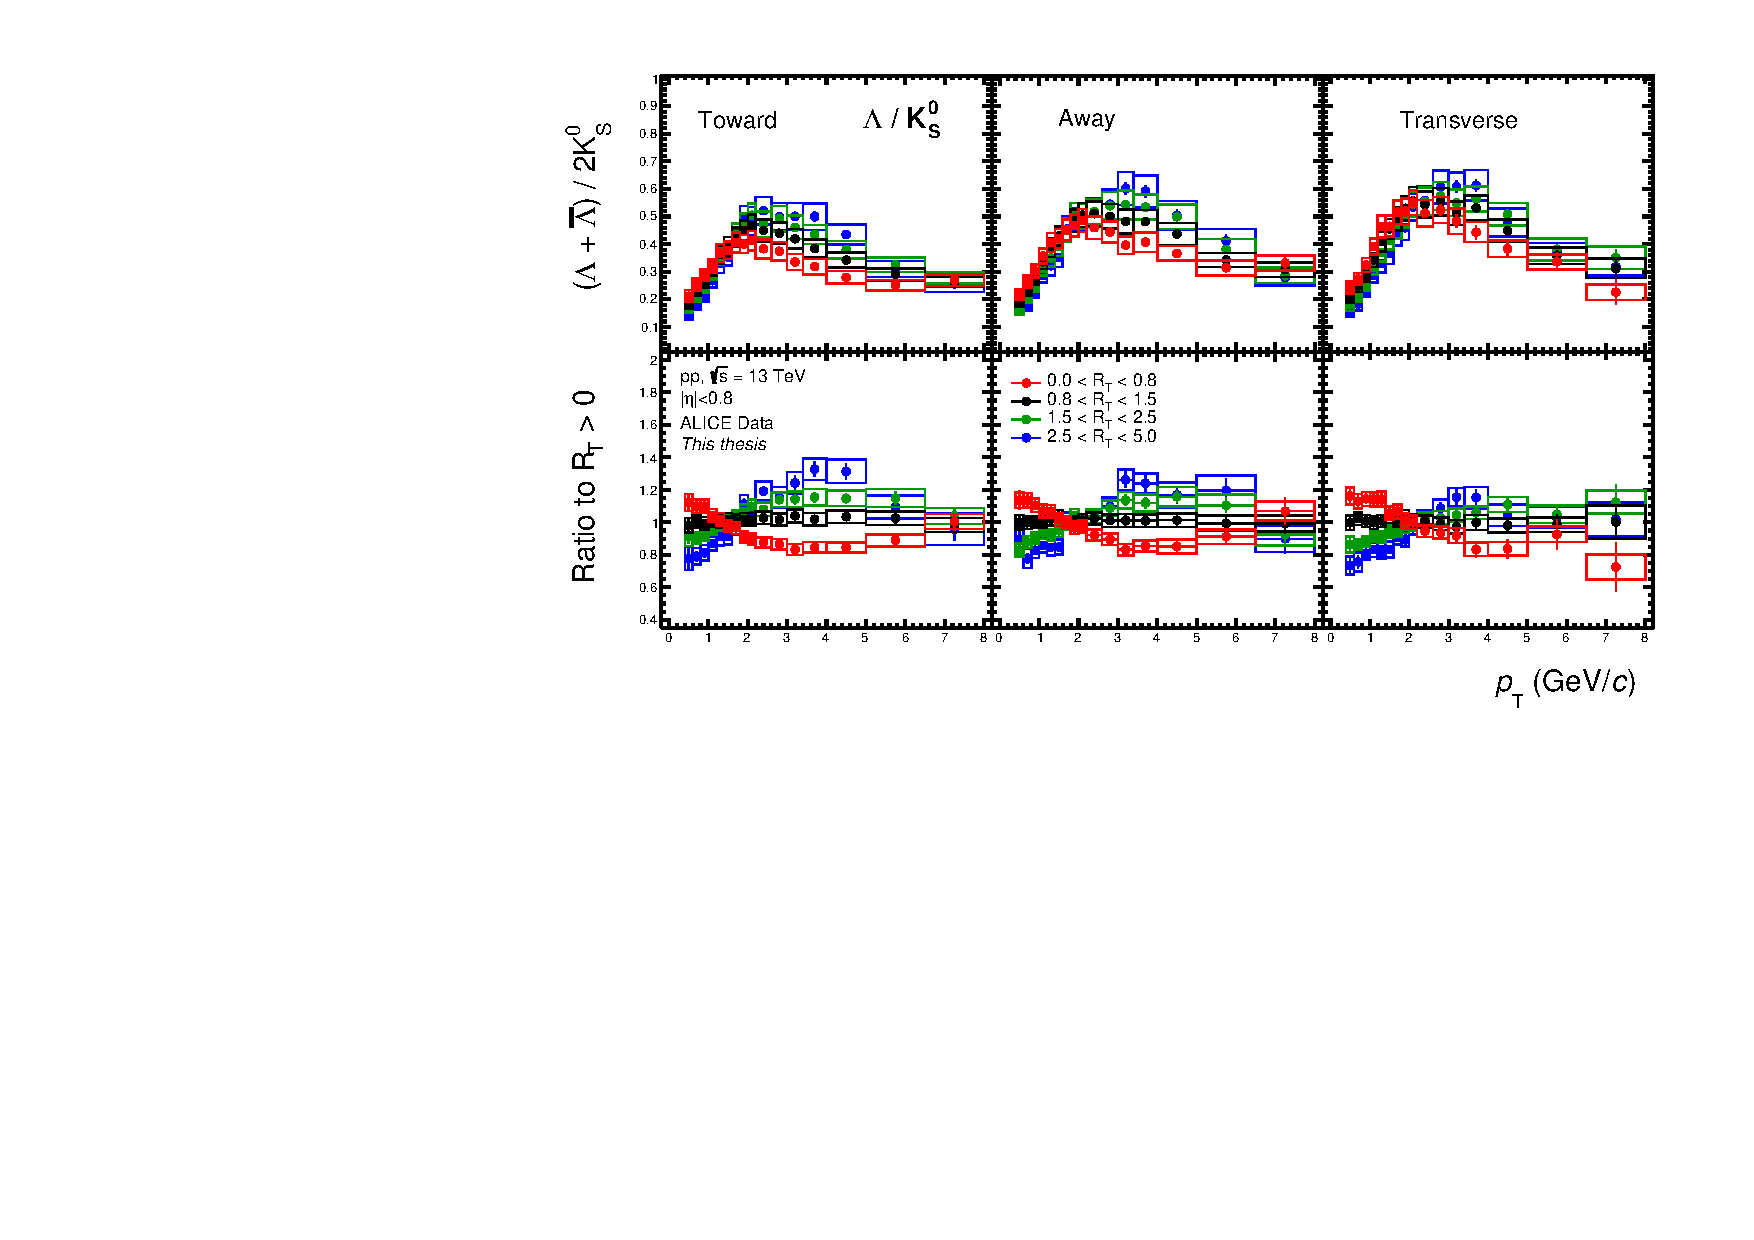
\includegraphics[width=.990\textwidth]{\imgpath/PtvRt_LtoK_K0s.pdf}}\\
\subfloat[][]{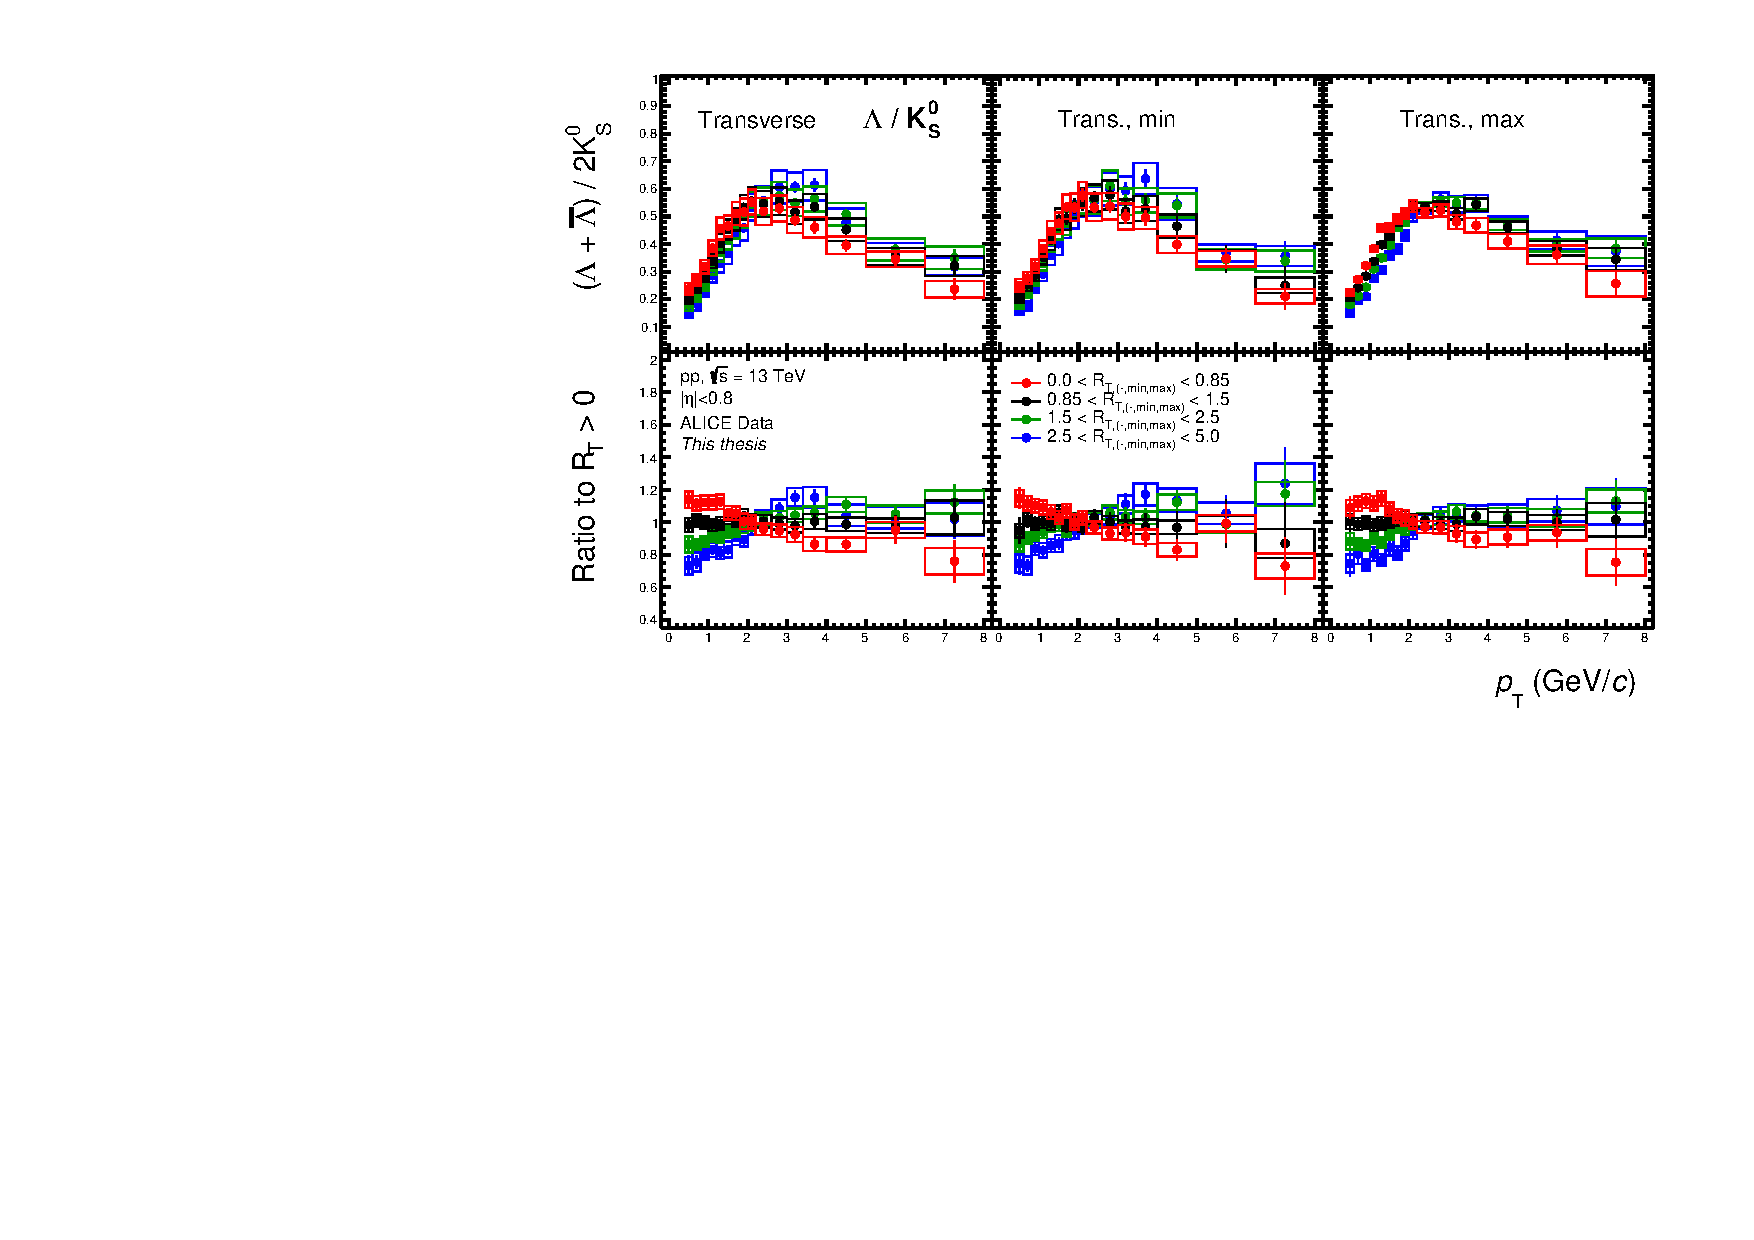
\includegraphics[width=.990\textwidth]{\imgpath/PtvRt_LtoK2_K0s.pdf}}\\
\caption{Baryon-to-meson ratios of \pt spectra \ltok for different \RT/\RTmin/\RTmax intervals in pp collisions at \sppt{13} in \textbf{(a)} Toward, Away, and Transverse, \textbf{(b)} Transverse, Transverse-min, and Transverse-max regions. The bottom panels display ratios to the \RT/\RTmin/\RTmax-integrated cases. The error bars represent statistical uncertainties and the rectangles show the systematic uncertainties.}
\label{fig:rt:LtoK}
\end{figure}


\begin{figure}[H]%
\subfloat[][]{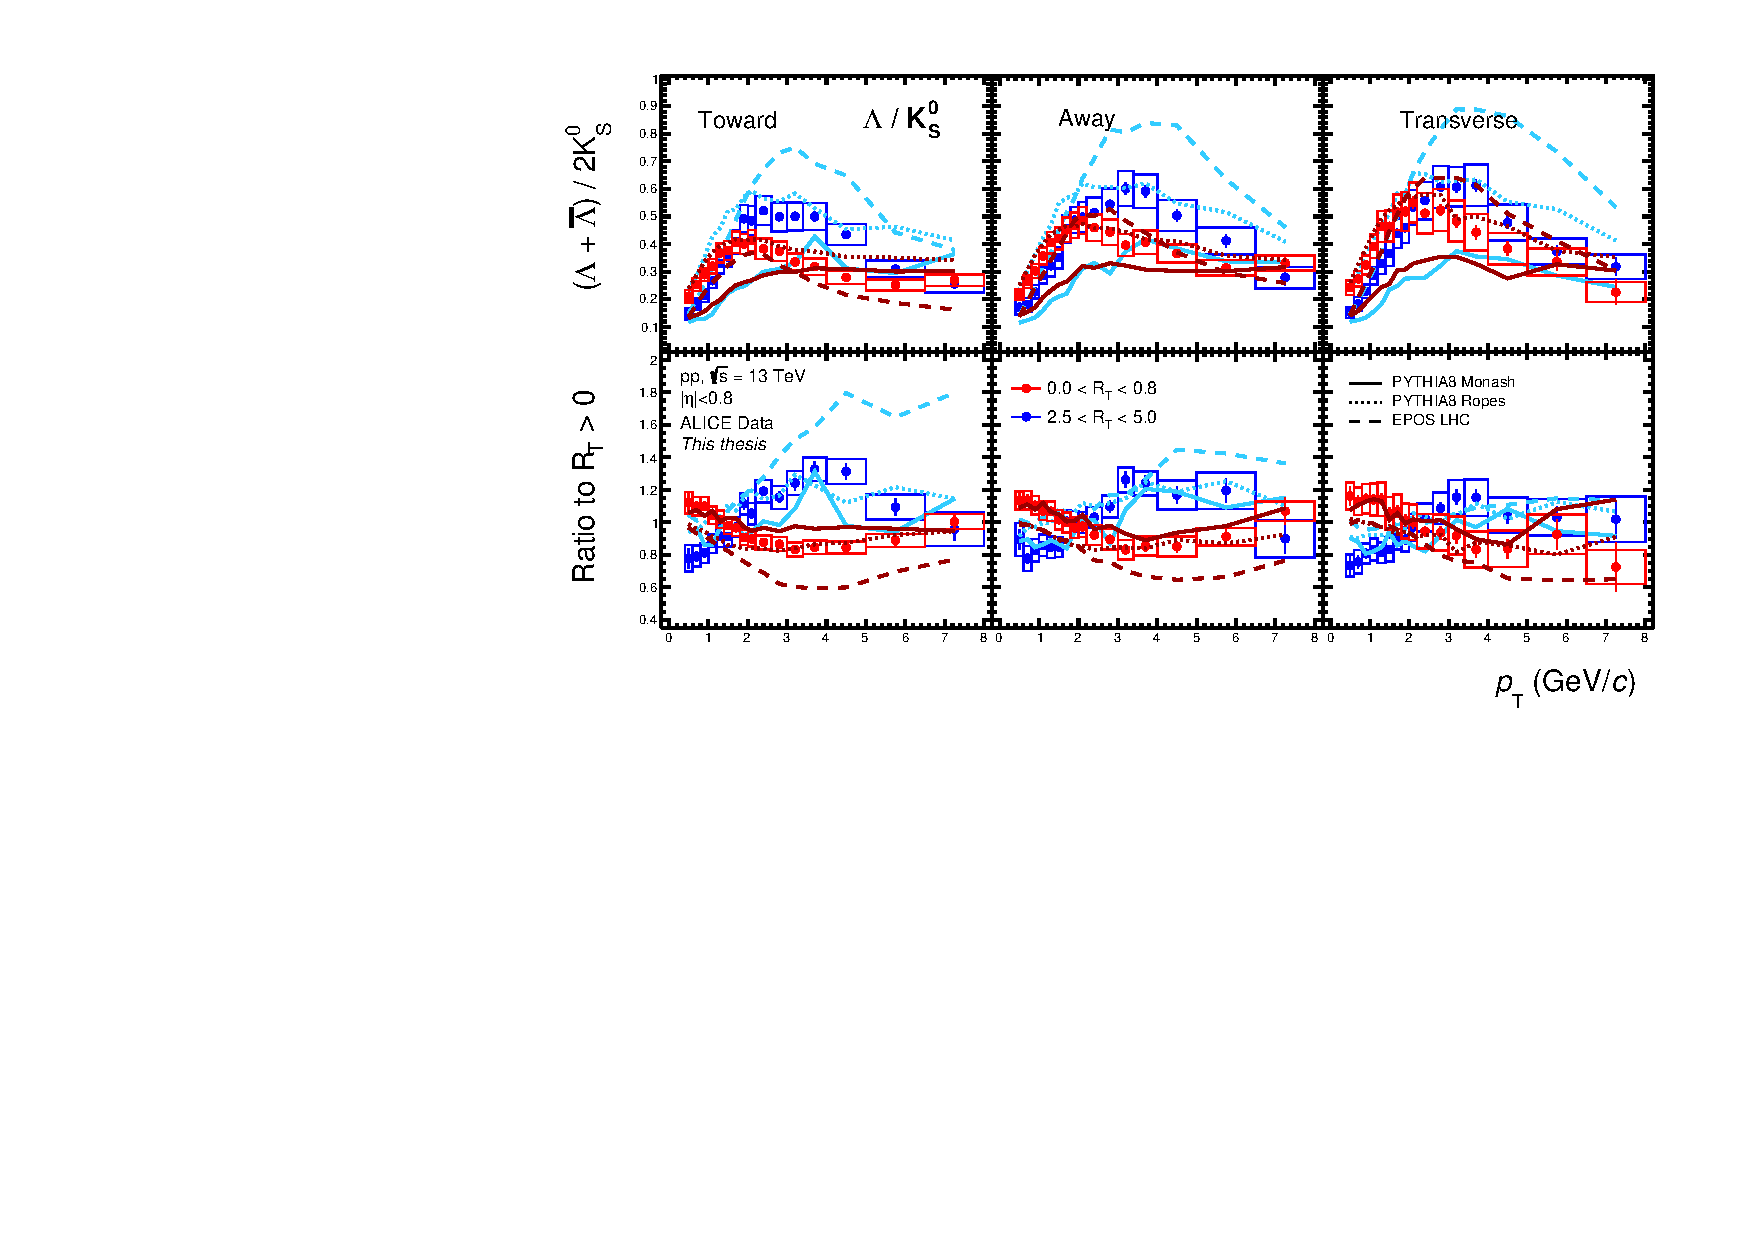
\includegraphics[width=.990\textwidth]{\imgpath/PtvRt_LtoKMC_K0s.pdf}}\\
\subfloat[][]{\includegraphics[width=.990\textwidth]{\imgpath/PtvRt_LtoKMC2_K0s.pdf}}\\
\caption{Baryon-to-meson ratios of \pt spectra \ltok for different \RT/\RTmin/\RTmax intervals in pp collisions at \sppt{13} in \textbf{(a)} Toward, Away, and Transverse, \textbf{(b)} Transverse, Transverse-min, and Transverse-max regions, compared with MC predictions. The bottom panels display ratios to the \RT/\RTmin/\RTmax-integrated cases. The error bars represent statistical uncertainties and the rectangles show the systematic uncertainties.}
\label{fig:rt:LtoKMC}
\end{figure}

\section{Integrated yields}

Finally, in Fig.~\ref{fig:rt:yield}, the integrated yields of \KOs and \LA are shown as a function of \RT, \RTmin, and \RTmax. The yields are self-normalised, similar to other multiplicity-dependent particle production measurements by ALICE. Using the same approach as in the \SOPT measurement, for the \VOs, the reported \pt range is used to integrate the yields, rather than extrapolating. The yields are then compared to data on pions and protons, as well as model predictions.

The yields of \KOs and \LA increase with \RT, but at a slower rate than the underlying UE activity (same rate would correspond to $y=x$). The increase of \LA with \RT appears to be somewhat faster than \KOs, which is in contrast to similar measurements using forward-rapidity event activity classifier \cite{adamEnhancedProductionMultistrange2017}. The largest increase in yields is observed in the Transverse and Transverse-max regions, with the Transverse-min region showing a slightly slower increase. In the Toward and Away regions, the increase in yields appears to be slower than linear.

When comparing the yields of charged particles \cite{vazquezruedaStudyProductionPp2022}, the effect of decoupling the neutral \KOs and \LA from the \NT in the Transverse region is evident. There is also slight, albeit systematic evidence for strangeness enhancement in the Toward and Away regions, with \KOs increasing slightly faster than $\pi$ and \LA slightly faster than $\mathrm{p}$. However, the uncertainties are significant, and strong conclusions cannot be drawn.

Based on the selected models, Pythia Monash and Pythia Ropes predict values that are consistent with the experimental data. EPOS LHC is also consistent in the Transverse regions but exhibits a faster rise with \RT than what is observed. In addition, it is less sensitive to the choice of regions compared to the other models.

\begin{figure}[H]%
\subfloat[][]{\includegraphics[width=.990\textwidth]{\imgpath/PtvRt_YieldPiKp_L.pdf}}\\
\subfloat[][]{\includegraphics[width=.990\textwidth]{\imgpath/PtvRt_Yield_L.pdf}}\\
\caption{Self-normalised yields of \KOs and \LA+\AL as a function of \RT/\RTmin/\RTmax, the self-normalised mid-rapidity underlying event activity, compared with \textbf{(a)} charged particles \cite{vazquezruedaStudyProductionPp2022} and \textbf{(b)} MC predictions. The \KOs and \LA+\AL yields are determined by integration in the reported \pt range. Datapoints are centered to the median \RT values, and not $\langle \RT \rangle$, of the given intervals. Statistical and systematic uncertainties are indicated by vertical error bars and boxes, respectively. }
\label{fig:rt:yield}
\end{figure}




